%%%%%%%%%%%%%%%%%%%%%%%%%%%%%%%%%%%%%%%%%%%%%%%%%%%%%%
\section{Welcome to HTCondor}  
%
% .... or alternatively called the 'warm fuzzies' section
% <smirk>  
% 
%
% Warning: much of what you are about to read was very 
% hastily written by a very tired Todd.... Good Luck.  
%%%%%%%%%%%%%%%%%%%%%%%%%%%%%%%%%%%%%%%%%%%%%%%%%%%%%

\label{sec:usermanual}
\index{HTCondor!user manual|(}
\index{user manual|(}
HTCondor is developed by
the Center for High Throughput Computing at the University of Wisconsin-Madison (UW-Madison), and
was first installed as a production system in the UW-Madison Computer
Sciences department more than 15 years ago. HTCondor pools have since
served as a major source of computing cycles to UW faculty and students.
For many, it has revolutionized the role computing plays in their
research. An increase of one, and sometimes even two, orders of
magnitude in the computing throughput of a research organization can
have a profound impact on research size, complexity, and scope. 
Over the years, the project, and now the Center for High Throughput Computing 
have established collaborations with scientists
from around the world, and have provided them with access to many
cycles. One scientist consumed 100 CPU years!

%%%%%%%%%%%%%%%%%%%%%%%%%%%%%%%%%%%%%%%%%%%%%%%%%%%%%%%
\section{Introduction}
%%%%%%%%%%%%%%%%%%%%%%%%%%%%%%%%%%%%%%%%%%%%%%%%%%%%%%%

In a nutshell, HTCondor is a specialized batch system 
\index{batch system}
for managing compute-intensive jobs.
Like most batch systems, HTCondor provides a
queuing mechanism, scheduling policy, priority scheme, and resource
classifications.  Users submit their compute jobs to HTCondor, HTCondor puts
the jobs in a queue, runs them, and then informs the user as to the
result.

Batch systems normally operate only with dedicated machines.  Often 
termed compute servers, these dedicated machines are typically owned by
one organization and dedicated to the sole purpose of running compute
jobs.  HTCondor can schedule jobs on dedicated machines.  But unlike traditional 
batch systems, HTCondor is also designed to effectively 
utilize non-dedicated machines to run jobs.  By being told to only
run compute jobs on machines which are currently not being used (no keyboard
activity, low load average, etc.), HTCondor can
effectively harness otherwise idle machines throughout a pool of machines.
This is important because often times the amount of
compute power represented by the aggregate total of all the non-dedicated 
desktop workstations sitting on people's desks throughout the
organization is far greater than the compute power of a dedicated
central resource.

HTCondor has several unique capabilities at its disposal which are geared 
toward effectively utilizing non-dedicated resources that are not owned or
managed by a centralized resource. These include transparent process
checkpoint and migration, remote system calls, and ClassAds.
Read section~\ref{sec:what-is-condor} for a general 
discussion of these features before reading any further.


%%%%%%%%%%%%%%%%%%%%%%%%%%%%%%%%%%%%%%%%%%%%%%%%%%%%%%%%
\section{Matchmaking with ClassAds}
\label{sec:matchmaking-with-classads}
%%%%%%%%%%%%%%%%%%%%%%%%%%%%%%%%%%%%%%%%%%%%%%%%%%%%%%%%

Before you learn about how to submit a job, it is important to
understand how HTCondor allocates resources. 
\index{HTCondor!resource allocation}
Understanding the
unique framework by which HTCondor matches submitted jobs with machines is
the key to getting the most from HTCondor's scheduling algorithm. 

HTCondor simplifies job submission by acting as a matchmaker of ClassAds.
HTCondor's ClassAds
\index{ClassAd}
are analogous to the classified advertising section of the
newspaper. Sellers advertise specifics about what they have to sell,
hoping to attract a buyer. Buyers may advertise specifics about what
they wish to purchase. Both buyers and sellers list constraints that
need to be satisfied.
For instance, a buyer has a maximum spending limit, 
and a seller requires a minimum purchase price.
Furthermore, both want to rank requests to their own advantage.
Certainly a seller would rank
one offer of \$50 dollars higher than a different
offer of \$25.
In HTCondor, users submitting
jobs can be thought of as buyers of compute resources and machine owners
are sellers. 

All machines in a HTCondor pool advertise their attributes,
\index{ClassAd!attributes}
such as
available memory, CPU type and speed, virtual memory size, current
load average, along with other static and dynamic properties.
This machine ClassAd
\index{ClassAd!machine}
also advertises under what conditions it is
willing to run a HTCondor job and what type of job it would prefer. These
policy attributes can reflect the individual terms and preferences by
which all the different owners have graciously allowed their machine to
be part of the HTCondor pool. 
You may
advertise that your machine is only willing to run jobs at night
and when there is no keyboard activity on your machine.
In addition, you may
advertise a preference (rank) for running jobs submitted by you
or one of your co-workers. 

Likewise, when submitting a job, you specify a ClassAd with
your requirements and preferences.
The ClassAd
\index{ClassAd!job}
includes the
type of machine you  wish to use. For instance, perhaps you are
looking for the fastest floating point performance available.
You want HTCondor to rank available machines
based upon floating point performance. Or, perhaps you
care only that the machine has a minimum of 128 Mbytes of RAM.
Or, perhaps you will
take any machine you can get! These job attributes and requirements
are bundled up into a job ClassAd.

HTCondor plays the role of a matchmaker by continuously reading
all the job ClassAds and all the machine ClassAds, 
matching and ranking job ads with machine ads.
HTCondor makes certain that all
requirements in both ClassAds are satisfied. 

%%%%%
\subsection{Inspecting Machine ClassAds with \condor{status}}
%%%%%

\index{HTCondor commands!condor\_status}
Once HTCondor is installed,
you will get a feel for what
a machine ClassAd does by trying
the \Condor{status} command.
Try the \Condor{status} command to get
a summary of information from
ClassAds about the resources available in your pool.
Type \Condor{status} and hit enter to see a summary 
similar to the following:
%\small       too big
%\tiny        too small
\footnotesize
\begin{verbatim}
Name               OpSys      Arch   State     Activity LoadAv Mem   ActvtyTime

amul.cs.wisc.edu   LINUX      INTEL  Claimed   Busy     0.990  1896  0+00:07:04
slot1@amundsen.cs. LINUX      INTEL  Owner     Idle     0.000  1456  0+00:21:58
slot2@amundsen.cs. LINUX      INTEL  Owner     Idle     0.110  1456  0+00:21:59
angus.cs.wisc.edu  LINUX      INTEL  Claimed   Busy     0.940   873  0+00:02:54
anhai.cs.wisc.edu  LINUX      INTEL  Claimed   Busy     1.400  1896  0+00:03:03
apollo.cs.wisc.edu LINUX      INTEL  Unclaimed Idle     1.000  3032  0+00:00:04
arragon.cs.wisc.ed LINUX      INTEL  Claimed   Busy     0.980   873  0+00:04:29
bamba.cs.wisc.edu  LINUX      INTEL  Owner     Idle     0.040  3032 15+20:10:19
\end{verbatim}
\normalsize
\Dots 


The \Condor{status} command has options that summarize machine ads 
in a variety of ways.
For example,
\begin{description}
\item[\Condor{status -available}] shows only machines which are
willing to run jobs now. 
\item[\Condor{status -run}] shows only machines
which are currently running jobs.  
\item[\Condor{status -long}] lists the machine ClassAds for all machines
in the pool.
\end{description}

Refer to the \Condor{status} command 
reference page located on page~\pageref{man-condor-status}
for a complete description of the \Condor{status} command.

The following shows a portion of a machine ClassAd
\index{ClassAd!machine example}
\index{machine ClassAd}
for a single machine: turunmaa.cs.wisc.edu. Some of the listed
attributes are used by
HTCondor for scheduling. Other attributes are for information purposes.
An important point is that \emph{any} of the attributes in a
machine ClassAd can be utilized at job submission time as part of a request
or preference on what machine to use. Additional attributes
can be easily added. For example, your site administrator can
add a physical location attribute to your machine ClassAds.

% condor_status -long turunmaa.cs.wisc.edu

\footnotesize
\begin{verbatim}
Machine = "turunmaa.cs.wisc.edu"
FileSystemDomain = "cs.wisc.edu"
Name = "turunmaa.cs.wisc.edu"
CondorPlatform = "$CondorPlatform: x86_rhap_5 $"
Cpus = 1
IsValidCheckpointPlatform = ( ( ( TARGET.JobUniverse == 1 ) == false ) || 
 ( ( MY.CheckpointPlatform =!= undefined ) && 
 ( ( TARGET.LastCheckpointPlatform =?= MY.CheckpointPlatform ) || 
 ( TARGET.NumCkpts == 0 ) ) ) )
CondorVersion = "$CondorVersion: 7.6.3 Aug 18 2011 BuildID: 361356 $"
Requirements = ( START ) && ( IsValidCheckpointPlatform )
EnteredCurrentActivity = 1316094896
MyAddress = "<128.105.175.125:58026>"
EnteredCurrentState = 1316094896
Memory = 1897
CkptServer = "pitcher.cs.wisc.edu"
OpSys = "LINUX"
State = "Owner"
START = true
Arch = "INTEL"
Mips = 2634
Activity = "Idle"
StartdIpAddr = "<128.105.175.125:58026>"
TargetType = "Job"
LoadAvg = 0.210000
CheckpointPlatform = "LINUX INTEL 2.6.x normal 0x40000000"
Disk = 92309744
VirtualMemory = 2069476
TotalSlots = 1
UidDomain = "cs.wisc.edu"
MyType = "Machine"
\end{verbatim}
\normalsize


%%%%%%%%%%%%%%%%%%%%%%%%%%%%%%%%%%%%%%%%%%%%%%%%%%%%%%%%%%%%%
\section{Running a Job: the Steps To Take}
%%%%%%%%%%%%%%%%%%%%%%%%%%%%%%%%%%%%%%%%%%%%%%%%%%%%%%%%%%%%%

\index{job!preparation}
The road to using HTCondor effectively is a short one.  The basics
are quickly and easily learned.

Here are all the steps needed to run a job using HTCondor.
\begin{description}

\item[Code Preparation.]
A job run under HTCondor must be able to 
run as a background batch job.
\index{job!batch ready}
HTCondor runs the program unattended and in the background. 
A program that runs in the background will not be able
to do interactive input and output.
HTCondor can redirect console output (\File{stdout} and \File{stderr})
and keyboard input (\File{stdin})
to and from files for the program.
Create any needed files that contain
the proper keystrokes needed for program input.
Make certain the program will run correctly with the files.

\item[The HTCondor Universe.]
HTCondor has several 
runtime environments (called a \Term{universe}) from which to choose.
Of the universes, two are likely choices when learning
to submit a job to HTCondor: the standard universe and the vanilla universe.
The standard universe allows a job running under HTCondor to
handle system calls by returning them to the machine where the
job was submitted.
The standard universe also provides the mechanisms necessary
to take a checkpoint and migrate a partially completed job,
should the machine on which the job is executing become
unavailable.
To use the standard universe, it is necessary to
relink the program with the HTCondor library using the
\Condor{compile} command.
The manual page for \Condor{compile} on page~\pageref{man-condor-compile} has details.

The vanilla universe provides a way to run jobs that cannot be
relinked.
There is no way to take a checkpoint or migrate a job executed
under the vanilla universe.
For access to input and output files, jobs must either use a shared
file system, or use HTCondor's File Transfer mechanism.

Choose a universe under which to run the HTCondor program,
and re-link the program if necessary.

\item[Submit description file.]
Controlling the details of a job submission is a
submit description file.
The file contains information
about the job such as what executable to run, the
files to use in place of \File{stdin} and \File{stdout}, and
the platform type required to run the program.
The number of times to run a program may be included;
it is simple to run the same program
multiple times with multiple data sets.

Write a submit description file to go with the job, using
the examples provided in section~\ref{sec:submitting}
for guidance.

\item[Submit the Job.]Submit the program to HTCondor with
the \Condor{submit} command.
\index{HTCondor commands!condor\_submit}

\end{description}

Once submitted, HTCondor does the rest toward running
the job.
Monitor the job's progress with the \Condor{q}
\index{HTCondor commands!condor\_q}
and \Condor{status} commands.
\index{HTCondor commands!condor\_status}
You may modify the order in which HTCondor will run your jobs with
\Condor{prio}. If desired, HTCondor can even inform you in a log file 
every time your job is checkpointed and/or migrated to a different machine. 

When your program completes, HTCondor will tell you
(by e-mail, if preferred) the exit status of your program and various
statistics about its performances, including time used and I/O performed.
If you are using a log file for the job (which is recommended) the exit
status will be recorded in the log file.
You can remove a job from the
queue prematurely with \Condor{rm}. 
\index{HTCondor commands!condor\_rm}


%%%%%%%%%%%%%%%%%%%%%%%%%%%%%%%%%%%%%%%%%%%%%%%%
\subsection{\label{sec:Choosing-Universe}
Choosing an HTCondor Universe}
%%%%%%%%%%%%%%%%%%%%%%%%%%%%%%%%%%%%%%%%%%%%%%%%

A \Term{universe} in HTCondor
\index{universe}
\index{HTCondor!universe}
defines an execution environment. 
HTCondor \VersionNotice\ supports several different
universes for user jobs:
\begin{itemize}
	\item Standard
	\item Vanilla
	\item Grid
	\item Java
	\item Scheduler
	\item Local
 	\item Parallel
 	\item VM
\end{itemize}

The \SubmitCmd{universe} under which a job runs
is specified in the submit description file.
If a universe is not specified,
the default is vanilla,
unless your HTCondor administrator has changed the default.
However, we strongly encourage you to specify the universe,
since the default can be changed by your HTCondor administrator,
and the default that ships with HTCondor has changed.

\index{universe!standard}
The standard universe provides migration and reliability, but has some
restrictions on the programs that can be run. 
\index{universe!vanilla}
The vanilla universe provides fewer services, but has very few
restrictions.
\index{universe!Grid}
The grid universe allows users to submit 
jobs using HTCondor's interface.
These jobs are submitted for execution on grid resources.
\index{universe!java}
\index{Java}
\index{Java Virtual Machine}
\index{JVM}
The java universe allows users to run jobs written for the
Java Virtual Machine (JVM).
The scheduler universe allows users to submit lightweight jobs
to be spawned by the program known as a daemon on the submit host itself.
\index{universe!parallel}
The parallel universe is for programs that require multiple machines
for one job.
See section~\ref{sec:Parallel} for more about the Parallel universe.
%\index{universe!Local}
%The local universe . . .
\index{universe!vm}
The vm universe allows users to run jobs where the job is
no longer a simple executable, but a disk image, facilitating
the execution of a virtual machine.

%%%%%%%%%%%%%%%%%%%%%%%%%%%%%%%%%%%%%%%%%%%%%%%%%%%%%%%%%%%%%%%%%%%%%%
\subsubsection{\label{sec:standard-universe}Standard Universe}
%%%%%%%%%%%%%%%%%%%%%%%%%%%%%%%%%%%%%%%%%%%%%%%%%%%%%%%%%%%%%%%%%%%%%%

\index{universe!standard}
In the standard universe, HTCondor provides \Term{checkpointing} and
\Term{remote system calls}.  These features make a job more reliable
and allow it uniform access to resources from anywhere in the pool.
To prepare a program as a standard universe job, it must be relinked
with \Condor{compile}.  Most programs can be prepared as a standard
universe job, but there are a few restrictions.

\index{checkpoint}
\index{checkpoint image}
HTCondor checkpoints a job at regular intervals.
A \Term{checkpoint image} is essentially a snapshot of the current
state of a job. 
If a job must be migrated from one machine to another,
HTCondor makes a checkpoint image, copies the image to the new machine,
and restarts the job continuing the job from where it left off.
If a machine should
crash or fail while it is running a job, HTCondor can restart the job on
a new machine using the most recent checkpoint image.
In this way, jobs
can run for months or years even in the face of occasional computer failures.

\index{remote system call}
\index{shadow}
Remote system calls make a job perceive that it is executing on its home
machine, even though the job may execute on many different machines over its
lifetime.
When a job runs on a remote machine, a second process, called
a \Condor{shadow} runs on the machine where the job was submitted.
\index{condor\_shadow}
\index{agents!condor\_shadow}
\index{HTCondor daemon!condor\_shadow}
\index{remote system call!condor\_shadow}
When the job attempts a system call, the \Condor{shadow} performs
the system call instead and sends the results to the remote
machine.
For example, if a job attempts to open a file that is
stored on the submitting machine,
the \Condor{shadow} will find the file,
and send the data to the machine where
the job is running.

To convert your program into a standard universe job, you must use
\Condor{compile} to relink it with the HTCondor libraries.
Put \Condor{compile} in front of your usual link command.
You do not need to modify the program's source code,
but you do need access to the unlinked object files.
A commercial program that is packaged as a single executable file cannot be
converted into a standard universe job.

For example, if you would have linked the job by executing:
\begin{verbatim}
% cc main.o tools.o -o program
\end{verbatim}

Then, relink the job for HTCondor with:
\begin{verbatim}
% condor_compile cc main.o tools.o -o program
\end{verbatim}

There are a few restrictions on standard universe jobs:

\input{user-man/limitations.tex}


%%%%%%%%%%%%
\subsubsection{Vanilla Universe}
%%%%%%%%%%%%

\index{universe!vanilla}
The vanilla universe in HTCondor is intended
for programs which cannot
be successfully re-linked.
Shell scripts are another case where the vanilla universe
is useful.
Unfortunately, jobs run under the vanilla universe cannot checkpoint or use
remote system calls. 
This has unfortunate consequences for a job that is partially
completed 
when the remote machine running a job must be returned
to its owner.
HTCondor has only two choices.  It can suspend the job, hoping to
complete it at a later time,
or it can give up and restart the job \emph{from the beginning} 
on another machine in the pool.

Since HTCondor's remote system call features cannot be used with the
vanilla universe, access to the job's input and output files becomes a
concern.
One option is for HTCondor to rely on a shared file system, such as NFS
or AFS. 
Alternatively, HTCondor has a mechanism for transferring files on behalf
of the user.
In this case, HTCondor will transfer any files needed by a job to the
execution site, run the job, and transfer the output back to the
submitting machine.

Under Unix, HTCondor presumes a shared file system for vanilla jobs. 
However, if a shared file system is unavailable, a user can enable the
HTCondor File Transfer mechanism.
On Windows platforms, the default is to use the File Transfer
mechanism.
For details on running a job with a shared file system, see
section~\ref{sec:shared-fs} on page~\pageref{sec:shared-fs}.
For details on using the HTCondor File Transfer mechanism, see 
section~\ref{sec:file-transfer} on page~\pageref{sec:file-transfer}.


%%%%%%%%%%%%
\subsubsection{Grid Universe}
%%%%%%%%%%%%

\index{universe!Grid}
The Grid universe in HTCondor is intended to provide the standard
HTCondor interface to users who wish to start jobs
intended for remote management systems.
Section~\ref{sec:GridUniverse} on page~\pageref{sec:GridUniverse}
has details on using the Grid universe.
The manual page for \Condor{submit}
on page~\pageref{man-condor-submit}
has detailed descriptions of
the grid-related attributes.

%%%%%%%%%%%%
\subsubsection{Java Universe}
%%%%%%%%%%%%

\index{universe!Java}

A program submitted to the Java universe may run on any sort of machine
with a JVM regardless of its location, owner, or JVM version.  HTCondor
will take care of all the details such as finding the JVM binary and
setting the classpath.

%%%%%%%%%%%%
\subsubsection{Scheduler Universe}
%%%%%%%%%%%%

\index{universe!scheduler}
\index{scheduler universe}

The scheduler universe allows users to submit lightweight jobs
to be run immediately, alongside the \Condor{schedd} daemon on the submit host
itself.
Scheduler universe jobs are not matched with a remote machine,
and will never be preempted.
The job's requirements expression is evaluated against the \Condor{schedd}'s
ClassAd.

Originally intended for meta-schedulers such as \Condor{dagman},
the scheduler universe can also be
used to manage jobs of any sort that must run on the submit host.

However, unlike the local universe, the scheduler
universe does not use a \Condor{starter} daemon to manage the job, and thus
offers limited features and policy support.  The local universe
is a better choice for most jobs which must run on the submit host, as
it offers a richer set of job management features, and is more
consistent with other universes such as the vanilla universe.
The scheduler universe may be retired in the future, in
favor of the newer local universe.


%%%%%%%%%%%%%%%%%%%%%%%%%%%%%%%%%%%%%%%%%%%%%%%%%%%%%%%%%%%%%%%%%%%%%%
\subsubsection{\label{sec:local-universe}Local Universe}
%%%%%%%%%%%%%%%%%%%%%%%%%%%%%%%%%%%%%%%%%%%%%%%%%%%%%%%%%%%%%%%%%%%%%%

\index{universe!local}
\index{local universe}
The local universe allows an HTCondor job to be submitted and
executed with different assumptions for the execution conditions
of the job.
The job does not wait to be matched with a machine.
It instead executes right away, on the machine where the job
is submitted.
The job will never be preempted.
The job's requirements expression is evaluated against the \Condor{schedd}'s
ClassAd.

%%%%%%%%%%%%
\subsubsection{Parallel Universe}
%%%%%%%%%%%%
\index{universe!parallel}
\index{parallel universe}
The parallel universe allows parallel programs, such as MPI jobs,
to be run within the opportunistic HTCondor environment.
Please see section~\ref{sec:Parallel} for more details.

%%%%%%%%%%%%
\subsubsection{VM Universe}
%%%%%%%%%%%%
\index{universe!vm}
\index{vm universe}
HTCondor facilitates the execution of VMware and Xen
virtual machines with the vm universe.

Please see section~\ref{sec:vmuniverse} for details.


%%%%%%%%%%%%%%%%%%%%%%%%%%%%%%%%%%%%%%%%%%%%%%%%%%%%%%%%%%%%%%
\section{\label{sec:submitting}Submitting a Job}
%%%%%%%%%%%%%%%%%%%%%%%%%%%%%%%%%%%%%%%%%%%%%%%%%%%%%%%%%%%%%%

\index{job!submitting}
A job is submitted for execution to HTCondor using the
\Condor{submit} command.
\index{HTCondor commands!condor\_submit}
\Condor{submit} takes as an argument the name of a
file called a submit description file.
\index{submit description file}
\index{file!submit description}
This file contains commands and keywords to direct the queuing of jobs.
In the submit description file, HTCondor finds everything it needs
to know about the job.  Items such as the name of the executable to run,
the initial working directory, and command-line arguments to the
program all go into
the submit description file.  \Condor{submit} creates a job
ClassAd based upon the information,
and HTCondor
works toward running the job.

\index{submit description file!contents of}
The contents of a submit description file have been designed to
save time for HTCondor users.
It is easy to submit multiple runs of a program to HTCondor
with a single submit description file.
To run the same program many times on
different input data sets, arrange the data files
accordingly so that each run reads its own input, and each run
writes its own output.
Each individual run may have its own initial
working directory, files mapped for \File{stdin}, \File{stdout},
\File{stderr}, command-line arguments, and
shell environment;  these are all specified in the submit description file.
A program that directly opens its own
files will read the file names to use either from \File{stdin}
or from the command line. 
A program that opens a static file, given by file name, every time
will need to use a separate subdirectory for the output of each run.

The \Condor{submit} manual page 
is on page~\pageref{man-condor-submit} and
contains a complete and full description of how to use \Condor{submit}.
It also includes descriptions of all the many commands that may be placed
into a submit description file.
In addition, the index lists entries for each command under the
heading of Submit Commands.

%%%%%%%%%%%%%%%%%%%%
\subsection{\label{sec:sample-submit-files}Sample submit description files}  
%%%%%%%%%%%%%%%%%%%%

In addition to the examples of submit description files given
here, there are more in the \Condor{submit} manual page.
\index{submit description file!examples|(}

\begin{description}
\item[Example 1]
\end{description}
Example 1 is one of the simplest submit description files possible. 
It queues up the program \Prog{myexe} for execution somewhere in the pool. 
Use of the vanilla universe is implied, as that is the default when
not specified in the submit description file.

An executable is compiled to run on a specific platform.
Since this submit description file does not specify a platform,
HTCondor will use its default,
which is to run the job on a machine which has the same architecture 
and operating system as the machine where \Condor{submit} is run
to submit the job. 

Standard input for this job will come from file \File{inputfile},
as specified by the \SubmitCmd{input} command,
and standard output for this job will go to file \File{outputfile},
as specified by the \SubmitCmd{output} command.
HTCondor expects to find these files in the current working directory,
as this job is submitted,
and the system will take care of getting the input file 
to where it needs to be when the job is executed,
as well as bring back the output results after job execution.

A log file, \File{myexe.log}, will also be produced that contains events
the job had during its lifetime inside of HTCondor.
When the job finishes, its exit conditions will be noted in the log file.
This file's contents are an excellent way to figure out what
happened to submitted jobs.
\begin{verbatim}
  ####################                                                    
  # 
  # Example 1                                                            
  # Simple HTCondor submit description file                                    
  #                                                                       
  ####################                                                    
                                                                          
  Executable   = myexe                                                    
  Log          = myexe.log                                                    
  Input        = inputfile
  Output       = outputfile
  Queue    
\end{verbatim}

\begin{description}
\item[Example 2]
\end{description}
Example 2 queues up one copy of the program \Prog{foo}
(which had been created by \Condor{compile})
for execution by HTCondor.
No \SubmitCmd{input}, \SubmitCmd{output}, or \SubmitCmd{error}
commands are given in the submit description file,
so \File{stdin}, \File{stdout}, and \File{stderr} will all refer to 
\File{/dev/null}.
The program may produce output by explicitly opening a file and writing to
it.
\begin{verbatim}
  ####################                                                    
  # 
  # Example 2                                                            
  # Standard universe submit description file
  #                                                                       
  ####################                                                    
                                                                          
  Executable   = foo                                                    
  Universe     = standard                                                    
  Log          = foo.log                                                    
  Queue    
\end{verbatim}

\begin{description}
\item[Example 3]
\end{description}

Example 3 queues two copies of the program \Prog{mathematica}. The
first copy will run in directory \File{run\_1}, and the second will run in
directory \File{run\_2} due to the \SubmitCmd{initialdir} command.
For each copy, 
\File{stdin} will be \File{test.data},
\File{stdout} will be \File{loop.out}, and
\File{stderr} will be \File{loop.error}.
Each run will read input and write output files within its own directory.
Placing data files in separate directories 
is a convenient way to organize data when
a large group of HTCondor jobs is to run.
The example file shows program submission of
\Prog{mathematica} as a vanilla universe job.
The vanilla universe is most often the right choice of universe
when the source and/or object code is not available.

The \SubmitCmd{request\_memory} command is included to ensure
that the \Prog{mathematica} jobs match with and then execute on
pool machines that provide at least 1 GByte of memory.

\begin{verbatim}
  ####################     
  #                       
  # Example 3: demonstrate use of multiple     
  # directories for data organization.      
  #                                        
  ####################                    
                                         
  executable     = mathematica          
  universe       = vanilla                   
  input          = test.data                
  output         = loop.out                
  error          = loop.error             
  log            = loop.log                                                    
  request_memory = 1 GB
                                  
  initialdir     = run_1         
  queue                         
                               
  initialdir     = run_2      
  queue                     
\end{verbatim}

\begin{description}
\item[Example 4]
\end{description}

The submit description file for Example 4 queues 150
\index{running multiple programs}
runs of program \Prog{foo} which has been compiled and linked for
Linux running on a 32-bit Intel processor.
This job requires HTCondor to run the program on machines which have
greater than 32 Mbytes of physical memory, 
and the \SubmitCmd{rank} command expresses a
preference to run each instance of the program 
on machines with more than 64 Mbytes.
It also advises HTCondor that this standard universe job will
use up to 28000 Kbytes of memory when running.
Each of the 150 runs of the program is given its own process number,
starting with process number 0.
So, files 
\File{stdin}, \File{stdout}, and \File{stderr} will
refer to \File{in.0}, \File{out.0}, and \File{err.0} for the first run
of the program,
\File{in.1}, \File{out.1},
and \File{err.1} for the second run of the program, and so forth.
A log file containing entries
about when and where HTCondor runs, checkpoints, and migrates processes for
all the 150 queued programs
will be written into the single file \File{foo.log}.
\begin{verbatim}
  ####################                    
  #
  # Example 4: Show off some fancy features including
  # the use of pre-defined macros.
  #
  ####################                                                    

  Executable     = foo                                                    
  Universe       = standard                                                    
  requirements   = OpSys == "LINUX" && Arch =="INTEL"     
  rank           = Memory >= 64
  image_size     = 28000
  request_memory = 32

  error   = err.$(Process)                                                
  input   = in.$(Process)                                                 
  output  = out.$(Process)                                                
  log     = foo.log

  queue 150
\end{verbatim}

\index{submit description file!examples|)}

%%%%%%%%%%%%%%%%%
\subsection{\label{sec:user-man-req-and-rank}About Requirements and Rank}
%%%%%%%%%%%%%%%%%

The 
\AdAttr{requirements} and \AdAttr{rank} commands in the submit description file
are powerful and flexible. 
\index{submit commands!requirements}
\index{requirements attribute}
\index{rank attribute}
\index{ClassAd attribute!requirements}
\index{ClassAd attribute!rank}
Using them effectively requires care, and this section presents
those details.

Both \AdAttr{requirements} and \AdAttr{rank} need to be specified 
as valid HTCondor ClassAd expressions, however, default values are set by the
\Condor{submit} program if these are not defined in the submit description file.
From the \Condor{submit} manual page and the above examples, you see
that writing ClassAd expressions is intuitive, especially if you
are familiar with the programming language C.  There are some
pretty nifty expressions you can write with ClassAds.
A complete description of ClassAds and their expressions
can be found in section~\ref{sec:classad-reference} on 
page~\pageref{sec:classad-reference}.

All of the commands in the submit description file are case insensitive, 
\emph{except} for the ClassAd attribute string values.
ClassAd attribute names are
case insensitive, but ClassAd string
values are \emph{case preserving}.

Note that the comparison operators
(\verb@<@, \verb@>@, \verb@<=@, \verb@>=@, and \verb@==@)
compare strings
case insensitively.  The special comparison operators 
\verb@=?=@ and \verb@=!=@
compare strings case sensitively.

A  \SubmitCmd{requirements} or \SubmitCmd{rank} command in
the submit description file may utilize attributes
that appear in a machine or a job ClassAd.
Within the submit description file (for a job) the
prefix \verb@MY.@ (on a ClassAd attribute name)
causes a reference to the job ClassAd attribute,
and the prefix \verb@TARGET.@ causes a reference to 
a potential machine or matched machine ClassAd attribute.

The \Condor{status} command displays
\index{HTCondor commands!condor\_status}
statistics about machines within the pool.
The \Opt{-l} option displays the
machine ClassAd attributes for all machines in the HTCondor pool.
The job ClassAds, if there are jobs in the queue, can be seen
with the \Condor{q -l} command.
This shows all the defined attributes for current jobs in the queue.

A list of defined ClassAd attributes for job ClassAds
is given in the unnumbered Appendix on 
page~\pageref{sec:Job-ClassAd-Attributes}.
A list of defined ClassAd attributes for machine ClassAds
is given in the unnumbered Appendix on 
page~\pageref{sec:Machine-ClassAd-Attributes}.


\subsubsection{\label{rank-examples}Rank Expression Examples}

\index{rank attribute!examples}
\index{ClassAd attribute!rank examples}
\index{submit commands!rank}
When considering the match between a job and a machine, rank is used
to choose a match from among all machines that satisfy the job's
requirements and are available to the user, after accounting for
the user's priority and the machine's rank of the job.
The rank expressions, simple or complex, define a numerical value
that expresses preferences.

The job's \Attr{Rank} expression evaluates to one of three values.
It can be UNDEFINED, ERROR, or a floating point value.
If \Attr{Rank} evaluates to a floating point value,
the best match will be the one with the largest, positive value.
If no \Attr{Rank} is given 
in the submit description file,
then HTCondor substitutes a default value of 0.0 when considering
machines to match.
If the job's \Attr{Rank} of a given machine evaluates
to UNDEFINED or ERROR,
this same value of 0.0 is used.
Therefore, the machine is still considered for a match,
but has no ranking above any other.

A boolean expression evaluates to the numerical value of 1.0
if true, and 0.0 if false.

The following \Attr{Rank} expressions provide examples to
follow.

For a job that desires the machine with the most available memory:
\begin{verbatim}
   Rank = memory
\end{verbatim}

For a job that prefers to run on a friend's machine
on Saturdays and Sundays:
\begin{verbatim}
   Rank = ( (clockday == 0) || (clockday == 6) )
          && (machine == "friend.cs.wisc.edu")
\end{verbatim}

For a job that prefers to run on one of three specific machines:
\begin{verbatim}
   Rank = (machine == "friend1.cs.wisc.edu") ||
          (machine == "friend2.cs.wisc.edu") ||
          (machine == "friend3.cs.wisc.edu")
\end{verbatim}

For a job that wants the machine with the best floating point
performance (on Linpack benchmarks):
\begin{verbatim}
   Rank = kflops
\end{verbatim}
This particular example highlights a difficulty with \Attr{Rank} expression
evaluation as currently defined.
While all machines have floating point processing ability,
not all machines will have the \Attr{kflops} attribute defined.
For machines where this attribute is not defined,
\Attr{Rank} will evaluate to the value UNDEFINED, and
HTCondor will use a default rank of the machine of 0.0.
The \Attr{Rank} attribute will only rank machines where
the attribute is defined.
Therefore, the machine with the highest floating point
performance may not be the one given the highest rank.

So, it is wise when writing a \Attr{Rank} expression to check
if the expression's evaluation will lead to the expected
resulting ranking of machines.
This can be accomplished using the \Condor{status} command with the
\Arg{-constraint} argument.  This allows the user to see a list of
machines that fit a constraint.
To see which machines in the pool have \Attr{kflops} defined,
use
\begin{verbatim}
condor_status -constraint kflops
\end{verbatim}
Alternatively, to see a list of machines where 
\AdAttr{kflops} is not defined, use
\begin{verbatim}
condor_status -constraint "kflops=?=undefined"
\end{verbatim}

For a job that prefers specific machines in a specific order:
\begin{verbatim}
   Rank = ((machine == "friend1.cs.wisc.edu")*3) +
          ((machine == "friend2.cs.wisc.edu")*2) +
           (machine == "friend3.cs.wisc.edu")
\end{verbatim}
If the machine being ranked is \Expr{friend1.cs.wisc.edu}, then the
expression
\begin{verbatim}
   (machine == "friend1.cs.wisc.edu")
\end{verbatim}
is true, and gives the value 1.0.
The expressions
\begin{verbatim}
   (machine == "friend2.cs.wisc.edu")
\end{verbatim}
and
\begin{verbatim}
   (machine == "friend3.cs.wisc.edu")
\end{verbatim}
are false, and give the value 0.0.
Therefore, \Attr{Rank} evaluates to the value 3.0.
In this way, machine \Expr{friend1.cs.wisc.edu} is ranked higher than
machine \Expr{friend2.cs.wisc.edu},
machine \Expr{friend2.cs.wisc.edu}
is ranked higher than 
machine \Expr{friend3.cs.wisc.edu},
and all three of these machines are ranked higher than others.

%%%%%%%%%%%% 

%%%%%%%%%%%% 
\subsection{\label{sec:shared-fs}
Submitting Jobs Using a Shared File System} 
%%%%%%%%%%%%
\index{job!submission using a shared file system}
\index{shared file system!submission of jobs}

If vanilla, java, or parallel universe
jobs are submitted without using the File Transfer mechanism, 
HTCondor must use a shared file system to access input and output
files. 
In this case, the job \emph{must} be able to access the data files
from any machine on which it could potentially run.

As an example, suppose a job is submitted from blackbird.cs.wisc.edu,
and the job requires a particular data file called
\File{/u/p/s/psilord/data.txt}.  If the job were to run on
cardinal.cs.wisc.edu, the file \File{/u/p/s/psilord/data.txt} must be
available through either NFS or AFS for the job to run correctly.

HTCondor allows users to ensure their jobs have access to the right
shared files by using the \AdAttr{FileSystemDomain} and
\AdAttr{UidDomain} machine ClassAd attributes.
These attributes specify which machines have access to the same shared
file systems.
All machines that mount the same shared directories in the same
locations are considered to belong to the same file system domain.
Similarly, all machines that share the same user information (in
particular, the same UID, which is important for file systems like
NFS) are considered part of the same UID domain.

The default configuration for HTCondor places each machine
in its own UID domain and file system domain, using the full host name of the
machine as the name of the domains.
So, if a pool \emph{does} have access to a shared file system,
the pool administrator \emph{must} correctly configure HTCondor 
such that all
the machines mounting the same files have the same
\AdAttr{FileSystemDomain} configuration.
Similarly, all machines that share common user information must be
configured to have the same \AdAttr{UidDomain} configuration.

When a job relies on a shared file system,
HTCondor uses the
\AdAttr{requirements} expression to ensure that the job runs
on a machine in the
correct \AdAttr{UidDomain} and \AdAttr{FileSystemDomain}.
In this case, the default \AdAttr{requirements} expression specifies
that the job must run on a machine with the same \AdAttr{UidDomain}
and \AdAttr{FileSystemDomain} as the machine from which the job
is submitted.
This default is almost always correct.
However, in a pool spanning multiple \AdAttr{UidDomain}s and/or
\AdAttr{FileSystemDomain}s, the user may need to specify a different
\AdAttr{requirements} expression to have the job run on the correct
machines.

For example, imagine a pool made up of both desktop workstations and a
dedicated compute cluster.
Most of the pool, including the compute cluster, has access to a
shared file system, but some of the desktop machines do not.
In this case, the administrators would probably define the
\AdAttr{FileSystemDomain} to be \File{cs.wisc.edu} for all the machines
that mounted the shared files, and to the full host name for each
machine that did not. An example is \File{jimi.cs.wisc.edu}.

In this example,
a user wants to submit vanilla universe jobs from her own desktop
machine (jimi.cs.wisc.edu) which does not mount the shared file system
(and is therefore in its own file system domain, in its own world).
But, she wants the jobs to be able to run on more than just her own
machine (in particular, the compute cluster), so she puts the program
and input files onto the shared file system.
When she submits the jobs, she needs to tell HTCondor to send them to
machines that have access to that shared data, so she specifies a
different \AdAttr{requirements} expression than the default:
\begin{verbatim}
   Requirements = TARGET.UidDomain == "cs.wisc.edu" && \
                  TARGET.FileSystemDomain == "cs.wisc.edu"
\end{verbatim}

\Warn If there is \emph{no} shared file system, or the HTCondor pool
administrator does not configure the \AdAttr{FileSystemDomain}
setting correctly (the default is that each machine in a pool is in
its own file system and UID domain), a user submits a job that cannot
use remote system calls (for example, a vanilla universe job), and the
user does not enable HTCondor's File Transfer mechanism, the job will
\emph{only} run on the machine from which it was submitted.


%%%%%%%%%%%% 
\subsection{\label{sec:file-transfer}
Submitting Jobs Without a Shared File System:
HTCondor's File Transfer Mechanism} 
%%%%%%%%%%%%

\index{job!submission without a shared file system}
\index{shared file system!submission of jobs without one}
\index{file transfer mechanism}
\index{transferring files}

HTCondor works well without a shared file system.
The HTCondor file transfer mechanism permits the user to select which files are
transferred and under which circumstances.
HTCondor can transfer any files needed by a job from
the machine where the job was submitted into a
remote scratch directory on the machine where the
job is to be executed.
HTCondor executes the job
and transfers output back to the submitting machine.
The user specifies which files and directories to transfer,
and at what point the output files should be copied back to the
submitting machine.
This specification is done within the job's submit description file.


%%%%%%%%%%%% 
\subsubsection{Specifying If and When to Transfer Files
\label{sec:file-transfer-if-when}}
%%%%%%%%%%%%

To enable the file transfer mechanism, place two commands
in the job's submit description file:
\SubmitCmd{should\_transfer\_files} and \SubmitCmd{when\_to\_transfer\_output}.
By default, they will be:

\begin{verbatim}
  should_transfer_files = IF_NEEDED
  when_to_transfer_output = ON_EXIT
\end{verbatim}

Setting the \SubmitCmd{should\_transfer\_files} command explicitly
enables or disables the file transfer mechanism.
The command takes on one of three possible values:
\begin{enumerate}

\item \verb@YES@: HTCondor transfers both the executable and the file
defined by the \SubmitCmd{input} command from the machine where the job is
submitted to the remote machine where the job is to be executed.
The file defined by the \SubmitCmd{output} command as well as any files
created by the execution of the job are transferred back to the machine
where the job was submitted.
When they are transferred and the directory location of the files
is determined by the command \SubmitCmd{when\_to\_transfer\_output}.

\item \verb@IF_NEEDED@: HTCondor transfers files if the job is
matched with and to be executed on a machine in a
different \Attr{FileSystemDomain} than the
one the submit machine belongs to, the same as if 
\verb@should_transfer_files = YES@.
If the job is matched with a machine in the local \Attr{FileSystemDomain},
HTCondor will not transfer files and relies
on the shared file system.

\item \verb@NO@: HTCondor's file transfer mechanism is disabled. 

\end{enumerate}

The \SubmitCmdNI{when\_to\_transfer\_output} command tells HTCondor when output
files are to be transferred back to the submit machine.
The command takes on one of two possible values:

\begin{enumerate}
\item \verb@ON_EXIT@: HTCondor transfers the file defined by the
\SubmitCmd{output} command,
 as well as any other files in the remote scratch directory created by the job,
back to the submit machine only when the job exits on its own.

\item \verb@ON_EXIT_OR_EVICT@: HTCondor behaves the same as described
for the value \verb@ON_EXIT@ when the job exits on its own.
However, if, and each time the job is evicted from a machine,
\emph{files are transferred back at eviction time}.  The files that
are transferred back at eviction time may include intermediate files
that are not part of the final output of the job.  Before the job
starts running again, all of the files that were stored when the job
was last evicted are copied to the job's new remote scratch
directory.

The purpose of saving files at eviction time is to allow the job to
resume from where it left off.
This is similar to using the checkpoint feature of the standard universe,
but just specifying \verb@ON_EXIT_OR_EVICT@ is not enough to make a job 
capable of producing or utilizing checkpoints.
The job must be designed to save and restore its state
using the files that are saved at eviction time.

The files that are transferred back at eviction time are not stored in
the location where the job's final output will be written when the job exits.
HTCondor manages these files automatically,
so usually the only reason for a user to worry about them 
is to make sure that there is enough space to store them.
The files are stored on the submit machine in a temporary directory within the
directory defined by the configuration variable \MacroNI{SPOOL}. 
The directory is named using the \Attr{ClusterId} and \Attr{ProcId} job
ClassAd attributes.  The directory name takes the form:
\begin{verbatim}
   <X mod 10000>/<Y mod 10000>/cluster<X>.proc<Y>.subproc0
\end{verbatim}
where \verb@<X>@ is the value of \Attr{ClusterId}, and 
\verb@<Y>@ is the value of \Attr{ProcId}. 
As an example, if job 735.0 is evicted, it will produce the directory
\begin{verbatim}
   $(SPOOL)/735/0/cluster735.proc0.subproc0
\end{verbatim}

\end{enumerate}

The default values for these two submit commands make sense as
used together.
If only \SubmitCmdNI{should\_transfer\_files} is set, 
and set to the value \Expr{NO}, 
then no output files will be transferred, and the value of
\SubmitCmdNI{when\_to\_transfer\_output} is irrelevant.
If only \SubmitCmdNI{when\_to\_transfer\_output} is set,
and set to the value \Expr{ON\_EXIT\_OR\_EVICT},
then the default value for an unspecified
\SubmitCmdNI{should\_transfer\_files} will be \Expr{YES}.

Note that the combination of
\begin{verbatim}
  should_transfer_files = IF_NEEDED
  when_to_transfer_output = ON_EXIT_OR_EVICT
\end{verbatim}
would produce undefined file access semantics.
Therefore, this combination is prohibited by \Condor{submit}.

%%%%%%%%%%%% 
\subsubsection{Specifying What Files to Transfer}
%%%%%%%%%%%%

% transfers before execution
If the file transfer mechanism is enabled,
HTCondor will transfer the following files before the job
is run on a remote machine.
\begin{enumerate}
  \item the executable, as defined with the \SubmitCmd{executable} command
  \item the input, as defined with the \SubmitCmd{input} command
  \item any jar files, for the \SubmitCmdNI{java} universe,
  as defined with the \SubmitCmd{jar\_files} command
\end{enumerate}
If the job requires other input files,
the submit description file should utilize the
\SubmitCmd{transfer\_input\_files} command.
This comma-separated list specifies any other files or directories that HTCondor is to
transfer to the remote scratch directory,
to set up the execution environment for the job before it is run.
These files are placed in the same directory as the job's executable.
For example:

\begin{verbatim}
  should_transfer_files = YES
  when_to_transfer_output = ON_EXIT
  transfer_input_files = file1,file2 
\end{verbatim}
This example explicitly enables the file transfer mechanism,
and it transfers the executable, the file specified by the \SubmitCmdNI{input}
command, any jar files specified by the \SubmitCmdNI{jar\_files} command,
and files \File{file1} and \File{file2}.

% transfers back after execution
If the file transfer mechanism is enabled,
HTCondor will transfer the following files from the execute machine
back to the submit machine after the job exits.
\begin{enumerate}
  \item the output file, as defined with the \SubmitCmdNI{output} command
  \item the error file, as defined with the \SubmitCmdNI{error} command
  \item any files created by the job in the remote scratch directory;
this only occurs for jobs other than \SubmitCmdNI{grid}
universe, and for HTCondor-C \SubmitCmdNI{grid} universe jobs;
directories created by the job within the remote scratch directory
are ignored for this automatic detection of files to be transferred.
\end{enumerate}

A path given for \SubmitCmdNI{output} and \SubmitCmdNI{error} commands represents
a path on the submit machine.  If no path is specified, the directory
specified with \SubmitCmd{initialdir} is used, and if that is not specified,
the directory from which the job was submitted is used.
At the time the job is submitted, zero-length files are created
on the submit machine, at the given path for the files defined by the  
\SubmitCmdNI{output} and \SubmitCmdNI{error} commands.
This permits job submission failure, if these files cannot be written by
HTCondor.

To \emph{restrict} the output files 
or permit entire directory contents to be transferred,
specify the exact list with  \SubmitCmd{transfer\_output\_files}.
Delimit the list of file names, directory names, or paths with commas.
When this list is defined, and any of the files or directories
do not exist as the job exits,
HTCondor considers this an error, and places the job on hold.
When this list is defined, automatic detection of output files created by
the job is disabled.
Paths specified in this list refer to locations on the execute
machine.  
The naming and placement of files and directories relies on the
term \Term{base name}.  
By example, the path \File{a/b/c} has the base name \File{c}.
It is the file name or directory name with all directories
leading up to that name stripped off.
On the submit machine, the transferred files or directories
are named using only the base name.
Therefore, each output file or directory must have a different name,
even if they originate from different paths.

For \SubmitCmdNI{grid} universe jobs other than than HTCondor-C grid jobs,
files to be transferred 
(other than standard output and standard error)
must be specified using \SubmitCmdNI{transfer\_output\_files}
in the submit description file, because automatic detection of new files
created by the job does not take place.

Here are examples to promote understanding of what files and
directories are transferred, and how they are named after transfer.
Assume that the job produces the following structure within the
remote scratch directory:
\begin{verbatim}
      o1
      o2
      d1 (directory)
          o3
          o4 
\end{verbatim}

If the submit description file sets
\begin{verbatim}
   transfer_output_files = o1,o2,d1
\end{verbatim}
then transferred back to the submit machine will be
\begin{verbatim}
      o1
      o2
      d1 (directory)
          o3
          o4 
\end{verbatim}
Note that the directory \File{d1} and all its contents are specified,
and therefore transferred.  
If the directory \File{d1} is not created by the job before exit,
then the job is placed on hold. 
If the directory \File{d1} is created by the job before exit,
but is empty, this is not an error.

If, instead, the submit description file sets
\begin{verbatim}
   transfer_output_files = o1,o2,d1/o3
\end{verbatim}
then transferred back to the submit machine will be
\begin{verbatim}
      o1
      o2
      o3
\end{verbatim}
Note that only the base name is used in the naming and placement
of the file specified with \File{d1/o3}.


%%%%%%%%%%%%
\subsubsection{File Paths for File Transfer}
%%%%%%%%%%%%

% Note: it might be nice to get the initialdir entry in
% the index to refer to something in here.

% Note: a Windows-based example would be good, too.

The file transfer mechanism specifies file names and/or paths on
both the file system of the submit machine and on the
file system of the execute machine.
Care must be taken to know which machine, submit or execute,
is utilizing the file name and/or path. 

Files in the \SubmitCmd{transfer\_input\_files} command
are specified as they are accessed on the submit machine.
The job, as it executes, accesses files as they are
found on the execute machine.

There are three ways to specify files and paths
for \SubmitCmd{transfer\_input\_files}:
\begin{enumerate}
\item Relative to the current working directory as the job is submitted,
if the submit command \SubmitCmd{initialdir} is not specified.
\item Relative to the initial directory, if the submit command 
\SubmitCmd{initialdir} is specified.
\item Absolute.
\end{enumerate}

Before executing the program, HTCondor copies the
executable, an input file as specified
by the submit command \SubmitCmd{input},
along with any input files specified 
by \SubmitCmd{transfer\_input\_files}.
All these files are placed into
a remote scratch directory on the execute machine,
in which the program runs.
Therefore,
the executing program must access input files relative to its
working directory.
Because all files and directories listed for transfer are placed into a single,
flat directory,
inputs must be uniquely named to
avoid collision when transferred.
A collision causes the last file in the list to
overwrite the earlier one.

Both relative and absolute paths may be used in
\SubmitCmd{transfer\_output\_files}.  Relative paths are relative to
the job's remote scratch directory on the execute machine.
When the files and directories are copied back to the submit machine, they
are placed in the job's initial working directory as the base name of
the original path.  An alternate name or path may be specified by using
\SubmitCmd{transfer\_output\_remaps}.

A job may create files outside the remote scratch directory
but within the file system of the execute machine,
in a directory such as \File{/tmp},
if this directory is guaranteed to exist and be
accessible on all possible execute machines.
However,
HTCondor will not automatically
transfer such files back after execution completes, nor will it clean
up these files.

Here are several examples to illustrate the use of file transfer.
The program executable is called \Prog{my\_program},
and it uses three command-line arguments as it executes: 
two input file names and an output file name.
The program executable and the submit description file 
for this job are located in directory
\File{/scratch/test}. 

Here is the directory tree as it exists on the submit machine,
for all the examples:
\begin{verbatim}
/scratch/test (directory)
      my_program.condor (the submit description file)
      my_program (the executable)
      files (directory)
          logs2 (directory)
          in1 (file)
          in2 (file)
      logs (directory)
\end{verbatim}

%--------------------------
\begin{description}
\item[Example 1]

This first example explicitly transfers input files.
These input files to be transferred
are specified relative to the directory where the job is submitted.
An output file specified in the \SubmitCmd{arguments} command, \File{out1},
is created when the job is executed.
It will be transferred back into the directory \File{/scratch/test}.

\footnotesize
\begin{verbatim}
# file name:  my_program.condor
# HTCondor submit description file for my_program
Executable      = my_program
Universe        = vanilla
Error           = logs/err.$(cluster)
Output          = logs/out.$(cluster)
Log             = logs/log.$(cluster)

should_transfer_files = YES
when_to_transfer_output = ON_EXIT
transfer_input_files = files/in1,files/in2

Arguments       = in1 in2 out1
Queue
\end{verbatim}
\normalsize

The log file is written on the submit machine, and is not involved
with the file transfer mechanism.
%--------------------------
\item[Example 2]

This second example is identical to Example 1,
except that absolute paths to the input files are specified,
instead of relative paths to the input files.

\footnotesize
\begin{verbatim}
# file name:  my_program.condor
# HTCondor submit description file for my_program
Executable      = my_program
Universe        = vanilla
Error           = logs/err.$(cluster)
Output          = logs/out.$(cluster)
Log             = logs/log.$(cluster)

should_transfer_files = YES
when_to_transfer_output = ON_EXIT
transfer_input_files = /scratch/test/files/in1,/scratch/test/files/in2

Arguments       = in1 in2 out1
Queue
\end{verbatim}
\normalsize

%--------------------------
\item[Example 3]

This third example illustrates the use of the 
submit command \SubmitCmd{initialdir}, and its effect
on the paths used for the various files.
The expected location of the 
executable is not affected by the 
\SubmitCmd{initialdir} command.
All other files
(specified by \SubmitCmd{input}, \SubmitCmd{output}, \SubmitCmd{error},
\SubmitCmd{transfer\_input\_files},
as well as files modified or created by the job
and automatically transferred back)
are located relative to the specified \SubmitCmd{initialdir}.
Therefore, the output file, \File{out1},
will be placed in the \verb@files@ directory.
Note that the \File{logs2} directory
exists to make this example work correctly.

\footnotesize
\begin{verbatim}
# file name:  my_program.condor
# HTCondor submit description file for my_program
Executable      = my_program
Universe        = vanilla
Error           = logs2/err.$(cluster)
Output          = logs2/out.$(cluster)
Log             = logs2/log.$(cluster)

initialdir      = files

should_transfer_files = YES
when_to_transfer_output = ON_EXIT
transfer_input_files = in1,in2

Arguments       = in1 in2 out1
Queue
\end{verbatim}
\normalsize

%--------------------------
\item[Example 4 -- Illustrates an Error]

This example illustrates a job that will fail.
The files specified using the
\SubmitCmd{transfer\_input\_files} command work
correctly (see Example 1).
However,
relative paths to files in the
\SubmitCmd{arguments} command
cause the executing program to fail.
The file system on the submission side may utilize
relative paths to files,
however those files are placed into the single,
flat, remote scratch directory on the execute machine.

\footnotesize
\begin{verbatim}
# file name:  my_program.condor
# HTCondor submit description file for my_program
Executable      = my_program
Universe        = vanilla
Error           = logs/err.$(cluster)
Output          = logs/out.$(cluster)
Log             = logs/log.$(cluster)

should_transfer_files = YES
when_to_transfer_output = ON_EXIT
transfer_input_files = files/in1,files/in2

Arguments       = files/in1 files/in2 files/out1
Queue
\end{verbatim}
\normalsize

This example fails with the following error:
\footnotesize
\begin{verbatim}
err: files/out1: No such file or directory.
\end{verbatim}
\normalsize

%--------------------------
\item[Example 5 -- Illustrates an Error]

As with Example 4,
this example illustrates a job that will fail.
The executing program's use of 
absolute paths cannot work.

\footnotesize
\begin{verbatim}
# file name:  my_program.condor
# HTCondor submit description file for my_program
Executable      = my_program
Universe        = vanilla
Error           = logs/err.$(cluster)
Output          = logs/out.$(cluster)
Log             = logs/log.$(cluster)

should_transfer_files = YES
when_to_transfer_output = ON_EXIT
transfer_input_files = /scratch/test/files/in1, /scratch/test/files/in2

Arguments = /scratch/test/files/in1 /scratch/test/files/in2 /scratch/test/files/out1
Queue
\end{verbatim}
\normalsize

The job fails with the following error:
\footnotesize
\begin{verbatim}
err: /scratch/test/files/out1: No such file or directory.
\end{verbatim}
\normalsize

%--------------------------
\item[Example 6]

This example illustrates a case
where the executing program creates an output file in a directory
other than within the remote scratch directory that the 
program executes within.
The file creation may or may not cause an error,
depending on the existence and permissions
of the directories on the remote file system.

The output file \File{/tmp/out1} is transferred back to the job's
initial working directory as \File{/scratch/test/out1}.

\footnotesize
\begin{verbatim}
# file name:  my_program.condor
# HTCondor submit description file for my_program
Executable      = my_program
Universe        = vanilla
Error           = logs/err.$(cluster)
Output          = logs/out.$(cluster)
Log             = logs/log.$(cluster)

should_transfer_files = YES
when_to_transfer_output = ON_EXIT
transfer_input_files = files/in1,files/in2
transfer_output_files = /tmp/out1

Arguments       = in1 in2 /tmp/out1
Queue
\end{verbatim}
\normalsize

\end{description}

%%%%%%%%%%%%
\subsubsection{Behavior for Error Cases}
%%%%%%%%%%%%
This section describes HTCondor's behavior for some error cases
in dealing with the transfer of files.
\begin{description}
\item[Disk Full on Execute Machine]
  When transferring any files from the submit machine to the remote scratch
  directory,
  if the disk is full on the execute machine,
  then the job is place on hold.
\item[Error Creating Zero-Length Files on Submit Machine]
  As a job is submitted, HTCondor creates zero-length files as placeholders
  on the submit machine for the files defined by 
  \SubmitCmd{output} and \SubmitCmd{error}.
  If these files cannot be created, then job submission fails.

  This job submission failure avoids having the job run to completion,
  only to be unable to transfer the job's output due to permission errors.
\item[Error When Transferring Files from Execute Machine to Submit Machine]
  When a job exits, or potentially when a job is evicted from an execute
  machine, one or more files may be transferred from the execute machine
  back to the machine on which the job was submitted.

  During transfer, if any of the following three similar types of errors occur,
  the job is put on hold as the error occurs.
  \begin{enumerate}
  \item If the file cannot be opened on the submit machine, for example
    because the system is out of inodes.
  \item If the file cannot be written on the submit machine, for example
    because the permissions do not permit it.
  \item If the write of the file on the submit machine fails, for example
    because the system is out of disk space.
  \end{enumerate}
\end{description}

%%%%%%%%%%%%
\subsubsection{File Transfer Using a URL \label{sec:file-transfer-by-URL}}
%%%%%%%%%%%%
\index{file transfer mechanism!input file specified by URL}
\index{file transfer mechanism!output file(s) specified by URL}
\index{URL file transfer}

Instead of file transfer that goes only between the submit machine
and the execute machine,
HTCondor has the ability to transfer files from a location specified
by a URL for a job's input file,
or from the execute machine to a location specified by a URL
for a job's output file(s).
This capability requires administrative set up, 
as described in section~\ref{sec:URL-transfer}.

The transfer of an input file is restricted to
vanilla and vm universe jobs only.
HTCondor's file transfer mechanism must be enabled.
Therefore, the submit description file for the job will define both
\SubmitCmd{should\_transfer\_files} and \SubmitCmd{when\_to\_transfer\_output}.
In addition, the URL for any files specified with a URL are
given in the \SubmitCmd{transfer\_input\_files} command.
An example portion of the submit description file for a job
that has a single file specified with a URL:

\footnotesize
\begin{verbatim}
should_transfer_files = YES
when_to_transfer_output = ON_EXIT
transfer_input_files = http://www.full.url/path/to/filename
\end{verbatim}
\normalsize

The destination file is given by the file name within the URL. 

For the transfer of the entire contents of the output sandbox,
which are all files that the job creates or modifies,
HTCondor's file transfer mechanism must be enabled.
In this sample portion of the submit description file,
the first two commands explicitly enable file transfer,
and the added \SubmitCmd{output\_destination} command provides
both the protocol to be used and the destination of the transfer.
\footnotesize
\begin{verbatim}
should_transfer_files = YES
when_to_transfer_output = ON_EXIT
output_destination = urltype://path/to/destination/directory
\end{verbatim}
\normalsize
Note that with this feature, no files are transferred back to the 
submit machine.  
This does not interfere with the streaming of output. 

If only a subset of the output sandbox should be transferred,
the subset is specified by further adding a submit command of the form:
\footnotesize
\begin{verbatim}
transfer_output_files = file1, file2
\end{verbatim}
\normalsize

%%%%%%%%%%%% 
\subsubsection{Requirements and Rank for File Transfer}
%%%%%%%%%%%%

\index{submit commands!requirements}
The \Attr{requirements} expression for a job must depend
on the \verb@should_transfer_files@ command.
The job must specify the correct logic to ensure that the job is matched
with a resource that meets the file transfer needs.
If no \Attr{requirements} expression is in the submit description file,
or if the expression specified does not refer to the
attributes listed below, \Condor{submit} adds an
appropriate clause to the \Attr{requirements} expression for the job.
\Condor{submit} appends these clauses with a logical AND, \verb@&&@,
to ensure that the proper conditions are met.
Here are the default clauses corresponding to the different values of
\verb@should_transfer_files@:

\begin{enumerate}

\item 
\verb@should_transfer_files = YES@ results in the addition of
the clause \verb@(HasFileTransfer)@.
  If the job is always going to transfer files, it is required to 
  match with a machine that has the capability to transfer files.

\item 
\verb@should_transfer_files = NO@ results in the addition of
  \verb@(TARGET.FileSystemDomain == MY.FileSystemDomain)@.
  In addition, HTCondor automatically adds the
  \Attr{FileSystemDomain} attribute to the job ClassAd, with whatever
  string is defined for the \Condor{schedd} to which the job is
  submitted.
  If the job is not using the file transfer mechanism, HTCondor assumes
  it will need a shared file system, and therefore, a machine in the
  same \Attr{FileSystemDomain} as the submit machine.

\item \verb@should_transfer_files = IF_NEEDED@ results in the addition of
\footnotesize
\begin{verbatim}
  (HasFileTransfer || (TARGET.FileSystemDomain == MY.FileSystemDomain))
\end{verbatim}
\normalsize
  If HTCondor will optionally transfer files, it must require
  that the machine is \emph{either} capable of transferring files
  \emph{or} in the same file system domain.

\end{enumerate}

To ensure that the job is matched to a machine with enough local disk
space to hold all the transferred files, HTCondor automatically adds the
\Attr{DiskUsage} job attribute.
This attribute includes the total
size of the job's executable and all input files to be transferred.
HTCondor then adds an additional clause to the \Attr{Requirements}
expression that states that the remote machine must have at least
enough available disk space to hold all these files:
\begin{verbatim}
  && (Disk >= DiskUsage)
\end{verbatim}

\index{submit commands!rank}
If \verb@should_transfer_files = IF_NEEDED@ and the job prefers
to run on a machine in the local file system domain
over transferring files,
but is still willing to allow the job to run remotely and transfer files,
the \Attr{Rank} expression works well.  Use:

\footnotesize
\begin{verbatim}
rank = (TARGET.FileSystemDomain == MY.FileSystemDomain)
\end{verbatim}
\normalsize

The \Attr{Rank} expression is a floating point value,
so if other items are considered in ranking the possible machines this job
may run on, add the items:

\footnotesize
\begin{verbatim}
Rank = kflops + (TARGET.FileSystemDomain == MY.FileSystemDomain)
\end{verbatim}
\normalsize

The value of \Attr{kflops} can vary widely among machines,
so this \Attr{Rank} expression will likely not do as it intends.
To place emphasis on the job running in the same file system domain,
but still consider floating point speed among the machines 
in the file system domain,
weight the part of the expression that is matching the file system domains.
For example: 

\footnotesize
\begin{verbatim}
Rank = kflops + (10000 * (TARGET.FileSystemDomain == MY.FileSystemDomain))
\end{verbatim}
\normalsize

%%%%%%%%%%%% 

%%%%%%%%%%%% 
\subsection{Environment Variables}
%%%%%%%%%%%% 

\index{environment variables}
\index{execution environment}
The environment under which a job executes often contains
information that is potentially useful to the job.
HTCondor allows a user to both set and reference environment
variables for a job or job cluster.

Within a submit description file, the user may define environment
variables for the job's environment by using the 
\Opt{environment} command.
See within the \Condor{submit} manual page at
section~\ref{man-condor-submit-environment} for more details about this command.

The submitter's entire environment can be copied into the job
ClassAd for the job at job submission.
The \SubmitCmd{getenv} command within the submit description file
does this,
as described at section~\ref{man-condor-submit-getenv}.

If the environment is set with the \SubmitCmd{environment} command \emph{and}
\SubmitCmdNI{getenv} is also set to true, values specified with
\SubmitCmdNI{environment} override values in the submitter's environment,
regardless of the order of the \SubmitCmdNI{environment} and \SubmitCmdNI{getenv}
commands.

Commands within the submit description file may reference the
environment variables of the submitter as a job is submitted.
Submit description file commands use \verb@$ENV(EnvironmentVariableName)@
to reference the value of an environment variable.

HTCondor sets several additional environment variables for each executing
job that may be useful for the job to reference.

\begin{itemize}
\item \Env{\_CONDOR\_SCRATCH\_DIR}
\index{\_CONDOR\_SCRATCH\_DIR environment variable}
\index{environment variables!\_CONDOR\_SCRATCH\_DIR}
 gives the directory
where the job may place temporary data files. 
This directory is unique for every job that is run,
and its contents are deleted by HTCondor
when the job stops running on a machine, no matter how the job completes.

\item \Env{\_CONDOR\_SLOT}
\index{\_CONDOR\_SLOT environment variable}
\index{environment variables!\_CONDOR\_SLOT}
gives the name of the slot (for SMP machines), on which the job is run.
On machines with only a single slot, the value of this variable will be
\verb@1@, just like the \AdAttr{SlotID} attribute in the machine's
ClassAd.
This setting is available in all universes.
See section~\ref{sec:Configuring-SMP} for more details about SMP
machines and their configuration.

\item \Env{CONDOR\_VM}
\index{CONDOR\_VM environment variable}
\index{environment variables!CONDOR\_VM}
equivalent to \Env{\_CONDOR\_SLOT} described above, except that it is
only available in the standard universe.
\Note As of HTCondor version 6.9.3, this environment variable is no longer
used.
It will only be defined if the \Macro{ALLOW\_VM\_CRUFT} configuration
variable is set to \Expr{True}.

\item \Env{X509\_USER\_PROXY}
\index{X509\_USER\_PROXY environment variable}
\index{environment variables!X509\_USER\_PROXY}
gives the full path to the X.509 user proxy file if one is
associated with the job.  Typically, a user will specify
\SubmitCmd{x509userproxy} in the submit description file.
This setting is currently available in the
local, java, and vanilla universes.

\item \Env{\_CONDOR\_JOB\_AD}
\index{\_CONDOR\_JOB\_AD environment variable}
\index{environment variables!\_CONDOR\_JOB\_AD}
is the path to a file in the job's scratch directory which contains
the job ad for the currently running job.  The job ad is current
as of the start of the job, but is not updated during the running
of the job.  The job may read attributes and their values out of
this file as it runs, but any changes will not be acted on in any
way by HTCondor.  The format is the same as the output of the
\Condor{q}  \Opt{-l} command.  This environment variable may be particularly
useful in a USER\_JOB\_WRAPPER.

\item \Env{\_CONDOR\_MACHINE\_AD}
\index{\_CONDOR\_MACHINE\_AD environment variable}
\index{environment variables!\_CONDOR\_MACHINE\_AD}
is the path to a file in the job's scratch directory which contains
the machine ad for the slot the currently running job is using.  
The machine ad is current as of the start of the job, but is not updated during the running
of the job.  The format is the same as the output of the
\Condor{status}  \Opt{-l} command.

\item \Env{\_CONDOR\_JOB\_IWD}
\index{\_CONDOR\_JOB\_IWD environment variable}
\index{environment variables!\_CONDOR\_JOB\_IWD}
is the path to the initial working directory the job was born with.

\item \Env{\_CONDOR\_WRAPPER\_ERROR\_FILE}
\index{\_CONDOR\_WRAPPER\_ERROR\_FILE environment variable}
\index{environment variables!\_CONDOR\_WRAPPER\_ERROR\_FILE}
is only set when the administrator has installed a USER\_JOB\_WRAPPER.
If this file exists, HTCondor assumes that the job wrapper has failed
and copies the contents of the file to the StarterLog for the administrator
to debug the problem.

\end{itemize}



%%%%%%%%%%%% 
\subsection{Heterogeneous Submit: Execution on Differing Architectures} 
%%%%%%%%%%%%

\index{job!heterogeneous submit}
\index{running a job!on a different architecture}
\index{heterogeneous pool!submitting a job to}
If executables are available for the different platforms of machines
in the HTCondor pool,
HTCondor can be allowed the choice of a larger number of machines
when allocating a machine for a job.
Modifications to the submit description file allow this choice
of platforms.

A simplified example is a cross submission.
An executable is available for one platform, but
the submission is done from a different platform.
Given the correct executable, the \AdAttr{requirements} command in
the submit description file specifies the target architecture.
For example, an executable compiled for a 32-bit Intel processor
running  Windows Vista, submitted
from an Intel architecture running Linux would add the 
\AdAttr{requirement}
\begin{verbatim}
  requirements = Arch == "INTEL" && OpSys == "WINDOWS"
\end{verbatim}
Without this \AdAttr{requirement}, \Condor{submit}
will assume that the program is to be executed on
a machine with the same platform as the machine where the job
is submitted.

Cross submission works for all universes except \Expr{scheduler} and
\Expr{local}.
See section~\ref{sec:Grid-Matchmaking} for how matchmaking works in the
\Expr{grid} universe.
The burden is on the user to both obtain and specify
the correct executable for the target architecture.
To list the architecture and operating systems of the machines
in a pool, run \Condor{status}.

%%%%%%%%%%%% 
\subsubsection{Vanilla Universe Example for Execution on Differing Architectures} 
%%%%%%%%%%%%

A more complex example of a heterogeneous submission
occurs when a job may be executed on
many different architectures to gain full
use of a diverse architecture and operating system pool.
If the executables are available for the different architectures,
then a modification to the submit description file
will allow HTCondor to choose an executable after an
available machine is chosen.

A special-purpose Machine Ad substitution macro can be used in
string
attributes in the submit description file.
The macro has the form
\begin{verbatim}
  $$(MachineAdAttribute)
\end{verbatim}
The \$\$() informs HTCondor to substitute the requested 
\AdAttr{MachineAdAttribute} 
from the machine where the job will be executed.

An example of the heterogeneous job submission
has executables available for two platforms:
RHEL 3 on both 32-bit and 64-bit Intel processors.
This example uses \Prog{povray}
to render images using a popular free rendering engine.

The substitution macro chooses a specific executable after
a platform for running the job is chosen.
These executables must therefore be named based on the
machine attributes that describe a platform.
The executables named \begin{verbatim}
  povray.LINUX.INTEL
  povray.LINUX.X86_64
\end{verbatim}
will work correctly for the macro
\begin{verbatim}
  povray.$$(OpSys).$$(Arch)
\end{verbatim}

The executables or links to executables with this name
are placed into the initial working directory so that they may be
found by HTCondor. 
A submit description file that queues three jobs for this example:

\begin{verbatim}
  ####################
  #
  # Example of heterogeneous submission
  #
  ####################

  universe     = vanilla
  Executable   = povray.$$(OpSys).$$(Arch)
  Log          = povray.log
  Output       = povray.out.$(Process)
  Error        = povray.err.$(Process)

  Requirements = (Arch == "INTEL" && OpSys == "LINUX") || \
                 (Arch == "X86_64" && OpSys =="LINUX") 

  Arguments    = +W1024 +H768 +Iimage1.pov
  Queue 

  Arguments    = +W1024 +H768 +Iimage2.pov
  Queue 

  Arguments    = +W1024 +H768 +Iimage3.pov
  Queue 
\end{verbatim}

These jobs are submitted to the vanilla universe
to assure that once a job is started on a specific platform,
it will finish running on that platform.
Switching platforms in the middle of job execution cannot
work correctly.

There are two common errors made with the substitution macro.
The first is the use of a non-existent \AdAttr{MachineAdAttribute}.
If the specified \AdAttr{MachineAdAttribute} does not
exist in the machine's ClassAd, then HTCondor will place
the job in the held state until the problem is resolved.

The second common error occurs due to an incomplete job set up.
For example, the submit description file given above specifies
three available executables.
If one is missing, HTCondor reports back that an
executable is missing when it happens to match the
job with a resource that requires the missing binary.

%%%%%%%%%%%% 
\subsubsection{Standard Universe Example for Execution on Differing Architectures} 
%%%%%%%%%%%%

Jobs submitted to the standard universe may produce checkpoints.
A checkpoint can then be used to start up and continue execution
of a partially completed job.
For a partially completed job, the checkpoint and the job are specific
to a platform.
If migrated to a different machine, correct execution requires that
the platform must remain the same.

In previous versions of HTCondor, the author of the heterogeneous
submission file would need to write extra policy expressions in the
\AdAttr{requirements} expression to force HTCondor to choose the
same type of platform when continuing a checkpointed job.
However, since it is needed in the common case, this
additional policy is now automatically added
to the \AdAttr{requirements} expression.
The additional expression is added
provided the user does not use
\AdAttr{CkptArch} in the \AdAttr{requirements} expression.
HTCondor will remain backward compatible for those users who have explicitly
specified \AdAttr{CkptRequirements}--implying use of \AdAttr{CkptArch},
in their \AdAttr{requirements} expression.

The expression added when the attribute \AdAttr{CkptArch} is not specified 
will default to

\footnotesize
\begin{verbatim}
  # Added by HTCondor
  CkptRequirements = ((CkptArch == Arch) || (CkptArch =?= UNDEFINED)) && \
                      ((CkptOpSys == OpSys) || (CkptOpSys =?= UNDEFINED))

  Requirements = (<user specified policy>) && $(CkptRequirements)
\end{verbatim}
\normalsize

The behavior of the \AdAttr{CkptRequirements} expressions and its addition to
\AdAttr{requirements} is as follows.
The \AdAttr{CkptRequirements} expression guarantees correct operation
in the two possible cases for a job.
In the first case, the job has not produced a checkpoint.
The ClassAd attributes \Attr{CkptArch} and \Attr{CkptOpSys}
will be undefined, and therefore the meta operator (\verb@=?=@)
evaluates to true.
In the second case, the job has produced a checkpoint.
The Machine ClassAd is restricted to require further execution
only on a machine of the same platform.
The attributes \Attr{CkptArch} and \Attr{CkptOpSys}
will be defined, ensuring that the platform chosen for further
execution will be the same as the one used just before the
checkpoint.

Note that this restriction of platforms also applies to platforms where
the executables are binary compatible.

The complete submit description file for this example:

\begin{verbatim}
  ####################
  #
  # Example of heterogeneous submission
  #
  ####################

  universe     = standard
  Executable   = povray.$$(OpSys).$$(Arch)
  Log          = povray.log
  Output       = povray.out.$(Process)
  Error        = povray.err.$(Process)

  # HTCondor automatically adds the correct expressions to insure that the
  # checkpointed jobs will restart on the correct platform types.
  Requirements = ( (Arch == "INTEL" && OpSys == "LINUX") || \
                 (Arch == "X86_64" && OpSys == "LINUX") )

  Arguments    = +W1024 +H768 +Iimage1.pov
  Queue 

  Arguments    = +W1024 +H768 +Iimage2.pov
  Queue 

  Arguments    = +W1024 +H768 +Iimage3.pov
  Queue 
\end{verbatim}


%%%%%%%%%%%% 
\subsubsection{Vanilla Universe Example for Execution on Differing Operating Systems} 
%%%%%%%%%%%%

The addition of several related OpSys attributes assists in selection of specific operating systems and versions in heterogeneous pools.


\begin{verbatim}
  ####################
  #
  # Example of submission targeting RedHat platforms in a heterogeneous Linux pool
  #
  ####################

  universe     = vanilla
  Executable   = /bin/date
  Log          = distro.log
  Output       = distro.out
  Error        = distro.err

  Requirements = (OpSysName == "RedHat")

  Queue
\end{verbatim}


\begin{verbatim}
  ####################
  #
  # Example of submission targeting RedHat 6 platforms in a heterogeneous Linux pool
  #
  ####################

  universe     = vanilla
  Executable   = /bin/date
  Log          = distro.log
  Output       = distro.out
  Error        = distro.err

  Requirements = ( OpSysName == "RedHat" && OpSysMajorVersion == 6)

  Queue
\end{verbatim}


Here is a more compact way to specify a RedHat 6 platform.

\begin{verbatim}
  ####################
  #
  # Example of submission targeting RedHat 6 platforms in a heterogeneous Linux pool
  #
  ####################

  universe     = vanilla
  Executable   = /bin/date
  Log          = distro.log
  Output       = distro.out
  Error        = distro.err

  Requirements = ( OpSysAndVer == "RedHat6")

  Queue
\end{verbatim}

%%%%%%%%%%%%%%%%%%%%%%%%%%%%%%%%%%%%%%%%%%
\subsection{\label{sec:Request-GPUs}Jobs That Require GPUs}
%%%%%%%%%%%%%%%%%%%%%%%%%%%%%%%%%%%%%%%%%%
\index{GPUs!requesting GPUs for a job}
A job that needs GPUs to run identifies the number of GPUs needed
in the submit description file by adding the submit command
\begin{verbatim}
  request_GPUs = <n>
\end{verbatim}
where \Expr{<n>} is replaced by the integer quantity of GPUs required
for the job.
For example, a job that needs 1 GPU uses
\begin{verbatim}
  request_GPUs = 1
\end{verbatim}

Because there are different capabilities among GPUs, 
the job might need to further qualify which GPU of available ones
is required.
Do this by specifying or adding a clause to an existing 
\SubmitCmd{Requirements} submit command.
As an example, 
assume that the job needs a speed and capacity of a CUDA GPU
that meets or exceeds the value 1.2.
In the submit description file, place
\begin{verbatim}
  request_GPUs = 1
  requirements = (CUDACapability >= 1.2) && $(requirements:True)
\end{verbatim}

Access to GPU resources by an HTCondor job needs special configuration
of the machines that offer GPUs.
Details of how to set up the configuration are in
section~\ref{sec:GPU-resources}.


%%%%%%%%%%%%%%%%%%%%%%%%%%%%%%%%%%%%%%%%%%
%%%%%%%%%%%%%%%%%%%%%%%%%%%%%%%%%%%%%%%%%%%%%%%%%%%%%%%%%%%%%%%%%%%%%%
\subsection{\label{sec:Submit-Interactive}Interactive Jobs}
%%%%%%%%%%%%%%%%%%%%%%%%%%%%%%%%%%%%%%%%%%%%%%%%%%%%%%%%%%%%%%%%%%%%%%
\index{job!interactive}
\index{interactive jobs}

An \Term{interactive job} is a Condor job that is provisioned and
scheduled like any other vanilla universe Condor job 
onto an execute machine within the pool.
The result of a running interactive job is a shell prompt 
issued on the execute machine where the job runs.
The user that submitted the interactive job may then use the
shell as desired,
perhaps to interactively run an instance of what is to become
a Condor job.
This might aid in checking that the set up and execution
environment are correct,
or it might provide information on the RAM or disk space needed.
This job (shell) continues until the user logs out or any other
policy implementation causes the job to stop running.
A useful feature of the interactive job is that the users and jobs
are accounted for within Condor's scheduling and priority system.

Neither the submit nor the execute host for interactive
jobs may be on Windows platforms. 

The current working directory of the shell will be the
initial working directory of the running job.
The shell type will be the default for the user that submits
the job.
At the shell prompt, X11 forwarding is enabled.

Each interactive job will have a job ClassAd attribute of 
\begin{verbatim}
  InteractiveJob = True
\end{verbatim}

Submission of an interactive job specifies the option \Opt{-interactive}
on the \Condor{submit} command line.

A submit description file may be specified for this interactive job.
Within this submit description file, 
a specification of these 5 commands will be either ignored or altered:
\begin{enumerate}
\item \SubmitCmd{executable}
\item \SubmitCmd{transfer\_executable}
\item \SubmitCmd{arguments}
\item \SubmitCmd{universe}.  The interactive job is a vanilla universe job. 
\item \SubmitCmd{queue} \SubmitCmdNI{<n>}.  In this case the value of \SubmitCmdNI{<n>} is
ignored; exactly one interactive job is queued.
\end{enumerate}
The submit description file may specify anything else needed for
the interactive job, such as files to transfer.

If \emph{no} submit description file is specified for the job,
a default one is utilized as identified by the value of the
configuration variable \Macro{INTERACTIVE\_SUBMIT\_FILE}.

Here are examples of situations where interactive jobs may be
of benefit.
\begin{itemize}
\item An application that cannot be batch processed might be run
as an interactive job.
Where input or output cannot be captured in a file and the
executable may not be modified,
the interactive nature of the job may still be run on a pool
machine, and within the purview of Condor.
\item A pool machine with specialized hardware that requires
interactive handling can be scheduled with an interactive
job that utilizes the hardware.
\item The debugging and set up of complex jobs or environments
may benefit from an interactive session.
This interactive session provides the opportunity to run scripts 
or applications, 
and as errors are identified, 
they can be corrected on the spot.
\item Development may have an interactive nature,
and proceed more quickly when done on a pool machine.
It may also be that the development platforms required
reside within Condor's purview as execute hosts. 
\end{itemize}

%%%%%%%%%%%%%%%%%%%%%%%%%%%%%%%%%%%%%%%%%%

%%%%%%%%%%%%%%%%%%%%%%%%%%%%%%%%%%%%%%%%%%
\section{Managing a Job}
\input{user-man/managing.tex}
%%%%%%%%%%%%%%%%%%%%%%%%%%%%%%%%%%%%%%%%%%

%%%%%%%%%%%%%%%%%%%%%%%%%%%%%%%%%%%%%%%%
\section{\label{sec:Priorities}Priorities and Preemption}
%%%%%%%%%%%%%%%%%%%%%%%%%%%%%%%%%%%%%%%%

HTCondor has two independent priority controls: \Term{job}
priorities and \Term{user} priorities.  

\subsection{Job Priority}

\index{job!priority}
\index{priority!of a job}
Job priorities allow the assignment of a priority level to
each submitted HTCondor job in order to
control the order of their execution.
\index{HTCondor commands!condor\_prio}
To set a job priority, use the \Condor{prio} command;
see the example in section~\ref{sec:job-prio}, or the
command reference page on page~\pageref{man-condor-prio}.
Job priorities do not impact user priorities in any fashion.
A job priority can be any integer, and higher values are \emph{better}.

%%%%%%%%%%%%%%%%%%%%%%%%%%%%%%%%%%%%%%%%%%%%%%%%%%%%%%%%%%%%%%%%%%%%%%
\subsection{\label{sec:user-priority-explained}User priority}
%%%%%%%%%%%%%%%%%%%%%%%%%%%%%%%%%%%%%%%%%%%%%%%%%%%%%%%%%%%%%%%%%%%%%%

\index{preemption!priority}
\index{user!priority}
\index{priority!of a user}
Machines are allocated to users based upon a user's priority.
A lower numerical value for user priority means higher priority,
so a user with priority 5 will get more resources than
a user with priority 50.
User priorities in HTCondor can be examined with the \Condor{userprio}
command (see page~\pageref{man-condor-userprio}).
\index{HTCondor commands!condor\_userprio}
HTCondor administrators can set and change individual user priorities
with the same utility.

HTCondor continuously calculates the share of available machines that each
user should be allocated.    This share is inversely related to the ratio
between user priorities.
For example, a user with a priority of 10 will get twice as many
machines as a user with a priority of 20.
The priority of each individual user changes according to
the number of resources the individual is using.
Each user starts out with the best possible priority: 0.5.
If the number of machines a user currently has is greater than 
the user priority,
the user priority will worsen by numerically increasing over time.
If the number of machines is less then the priority,
the priority will improve by numerically decreasing over time. 
The long-term result is fair-share access across all users.
The speed at which HTCondor adjusts the priorities is
controlled with the configuration variable \Macro{PRIORITY\_HALFLIFE},
an exponential half-life value.
The default is one day.
If a user that has user priority of 100 and is
utilizing 100 machines removes all his/her jobs,
one day later that user's
priority will be 50, and two days later the priority will be 25.

HTCondor enforces that each user gets his/her fair share of machines
according to user priority both when allocating machines which become
available and by priority preemption of currently allocated machines.
For instance, if a low priority user is utilizing all available machines
and suddenly a higher priority user submits jobs, HTCondor will
immediately take a checkpoint and vacate jobs belonging to the lower priority
user. This will free up machines that HTCondor will then give over to the
higher priority user. HTCondor will not starve the lower priority user; it
will preempt only enough jobs so that the higher priority user's fair
share can be realized (based upon the ratio between user priorities). To
prevent thrashing of the system due to priority preemption, the HTCondor 
site administrator can define a \Macro{PREEMPTION\_REQUIREMENTS} expression in HTCondor's configuration.
The default expression that ships with HTCondor is configured to only preempt 
lower priority jobs that have run
for at least one hour. So in the previous example, in the worse case it
could take up to a maximum of one hour until the higher priority user
receives a fair share of machines.
For a general discussion of
limiting preemption,
please see
section \ref{sec:Disabling Preemption} of the Administrator's manual.

User priorities are keyed on \Expr{<username>@<domain>}, for example
\Expr{johndoe@cs.wisc.edu}. The domain name to use, if any, is configured by
the HTCondor site administrator.  Thus, user priority and therefore resource
allocation is not impacted by which machine the user submits from or
even if the user submits jobs from multiple machines.

\index{nice job}
\index{priority!nice job}
An extra feature is the ability to submit a job as
a \Term{nice} job (see page~\pageref{man-condor-submit-nice}).
Nice jobs artificially boost the user priority 
by ten million just for the nice job.
This effectively means that nice jobs will only run on
machines that no other HTCondor job (that is, non-niced job) wants.
In a similar fashion, an HTCondor administrator could set
the user priority of any specific HTCondor user very high.
If done, for example, with a guest account,
the guest could only use cycles not wanted by other users of the system.


%%%%%%%%%%%%%%%%%%%%%%%%%%%%%%%%%%%%%%%%%%%%%%%%%%%%%%%%%%%%%%%%%%%%%%
\subsection{\label{sec:Vacate-Explained}
Details About How HTCondor Jobs Vacate Machines}
%%%%%%%%%%%%%%%%%%%%%%%%%%%%%%%%%%%%%%%%%%%%%%%%%%%%%%%%%%%%%%%%%%%%%%

\index{vacate}
\index{preemption!vacate}
When HTCondor needs a job to vacate a machine for whatever reason, it
sends the job an asynchronous signal specified in the \AdAttr{KillSig}
attribute of the job's ClassAd.
The value of this attribute can be specified by
the user at submit time by placing the \Opt{kill\_sig} option in the
HTCondor submit description file.  

If a program wanted to do some special work when required
to vacate a machine, the program may set up a
signal handler to use a trappable signal as an indication
to clean up.
When submitting this job, this clean up signal is specified to be used with
\Opt{kill\_sig}.
Note that the clean up work needs to be quick.
If the job takes too long to go away, HTCondor
follows up with a SIGKILL signal which immediately terminates the
process.

\index{HTCondor commands!condor\_compile}
A job that is linked using \Condor{compile}
and is subsequently submitted into the standard universe, 
will checkpoint and exit upon receipt of a SIGTSTP signal.
Thus, SIGTSTP is
the default value for \AdAttr{KillSig} when submitting to the standard
universe.
The user's code may still checkpoint itself at any time
by calling one of the following functions exported by the HTCondor libraries:
\begin{description}
\item[\Procedure{ckpt()}] Performs a checkpoint and then returns.
\item[\Procedure{ckpt\_and\_exit()}] Checkpoints and exits; HTCondor will then
restart the process again later, potentially on a different machine.
\end{description}

For jobs submitted into the vanilla universe, the default value for
\AdAttr{KillSig} is SIGTERM,
the usual method to nicely terminate a Unix program.

%%%%%%%%%%%%%%%%%%%%%%%%%%%%%%%%%%%%%%%%%%%%%%%%%%%%%%%%%%%%%%%%%%%%%%

%%%%%%%%%%%%%%%%%%%%%%%%%%%%%%%%%%%%%%%%%%%%%%%%%%%%%%%%%%%%%%%%%%%%%%
\section{\label{sec:Java}Java Applications}
%%%%%%%%%%%%%%%%%%%%%%%%%%%%%%%%%%%%%%%%%%%%%%%%%%%%%%%%%%%%%%%%%%%%%%
\index{Java}

HTCondor allows users to access a wide variety of
machines distributed around the world.
The Java Virtual Machine (JVM)
\index{Java Virtual Machine}
\index{JVM}
provides a uniform platform on any machine, regardless of the
machine's architecture or operating system.
The HTCondor Java universe brings together these
two features to create a distributed, homogeneous computing environment.

Compiled Java programs can be submitted to HTCondor, and HTCondor
can execute the programs on any machine in the pool that will run
the Java Virtual Machine.


The \Condor{status} command can be used to see a list of
machines in the pool for which HTCondor can use the Java Virtual
Machine.

\footnotesize
\begin{verbatim}
% condor_status -java

Name               JavaVendor Ver    State     Activity LoadAv  Mem  ActvtyTime

adelie01.cs.wisc.e Sun Micros 1.6.0_ Claimed   Busy     0.090   873  0+00:02:46
adelie02.cs.wisc.e Sun Micros 1.6.0_ Owner     Idle     0.210   873  0+03:19:32
slot10@bio.cs.wisc Sun Micros 1.6.0_ Unclaimed Idle     0.000   118  7+03:13:28
slot2@bio.cs.wisc. Sun Micros 1.6.0_ Unclaimed Idle     0.000   118  7+03:13:28
...
\end{verbatim}
\normalsize

If there is no output from the
\Condor{status} command,
then HTCondor does not know the location details of the Java Virtual
Machine on machines in the pool,
or no machines have Java correctly installed.
In this case,
contact your system administrator or see section \ref{sec:java-install}
for more information on getting HTCondor to work together
with Java.

%%%%%
\subsection{A Simple Example Java Application}
%%%%%
\index{Java!job example}

Here is a complete, if simple, example.
Start with a simple Java program, \File{Hello.java}:

\begin{verbatim}
public class Hello {
        public static void main( String [] args ) {
                System.out.println("Hello, world!\n");
        }
}
\end{verbatim}

Build this program using your Java compiler.
On most platforms, this is
accomplished with the command
\begin{verbatim}
javac Hello.java
\end{verbatim}

Submission to HTCondor requires a submit description file.
If submitting where files are accessible using a
shared file system,
this simple submit description file works:

\begin{verbatim}
  ####################
  #
  # Example 1
  # Execute a single Java class
  #
  ####################

  universe       = java
  executable     = Hello.class
  arguments      = Hello
  output         = Hello.output
  error          = Hello.error
  queue
\end{verbatim}

The Java universe must be explicitly selected.

The main class of the program is given in the \SubmitCmd{executable} statement.
This is a file name which contains the entry point of the program.
The name of the main class (not a file name) must
be specified as the first argument to the program.

If submitting the job where a shared file system is \emph{not}
accessible,
the submit description file becomes:

\begin{verbatim}
  ####################
  #
  # Example 2
  # Execute a single Java class,
  # not on a shared file system
  #
  ####################

  universe       = java
  executable     = Hello.class
  arguments      = Hello
  output         = Hello.output
  error          = Hello.error
  should_transfer_files = YES
  when_to_transfer_output = ON_EXIT
  queue
\end{verbatim}
For more information about using HTCondor's file transfer mechanisms,
see section~\ref{sec:file-transfer}.

To submit the job, where the submit description file
is named \File{Hello.cmd}, 
execute 
\begin{verbatim}
condor_submit Hello.cmd
\end{verbatim}

To monitor the job, the commands \Condor{q} and \Condor{rm}
are used as with all jobs.

%%%%%
\subsection{Less Simple Java Specifications}
%%%%%

\begin{description}
\item[Specifying more than 1 class file.]
\index{Java!multiple class files}
For programs that 
consist of more than one \Code{.class} file,
identify the files in the submit description file:

\begin{verbatim}
executable = Stooges.class
transfer_input_files = Larry.class,Curly.class,Moe.class
\end{verbatim}

The \SubmitCmd{executable} command does not change.
It still identifies the class file that contains the program's
entry point.

\item[JAR files.]
\index{Java!using JAR files}
If the program consists of a large number of class files,
it may be easier to collect them all together into
a single Java Archive (JAR) file.
A JAR can be created with:

\footnotesize
\begin{verbatim}
% jar cvf Library.jar Larry.class Curly.class Moe.class Stooges.class
\end{verbatim}
\normalsize

HTCondor must then be told where to find the JAR as well
as to use the JAR. 
The JAR file that contains the entry point
is specified with the \SubmitCmd{executable} command.
All JAR files are specified with the \SubmitCmd{jar\_files}
command.
For this example that collected all the class files
into a single JAR file, the submit description file contains:

\begin{verbatim}
executable = Library.jar
jar_files = Library.jar
\end{verbatim}

Note that the JVM must know whether it is receiving JAR files
or class files.
Therefore, HTCondor must also be informed, in order to pass the
information on to the JVM.
That is why there is a difference in submit description file commands
for the two ways of specifying files (\SubmitCmd{transfer\_input\_files}
and \SubmitCmd{jar\_files}).

If there are multiple JAR files,
the \SubmitCmd{executable} command specifies the JAR file
that contains the program's entry point.
This file is also listed with the \SubmitCmd{jar\_files} command:
\begin{verbatim}
executable = sortmerge.jar
jar_files = sortmerge.jar,statemap.jar
\end{verbatim}

\item[Using a third-party JAR file.]
As HTCondor requires that all JAR files (third-party or not)
be available,
specification of a third-party JAR file is no different than
other JAR files.
If the sortmerge example above also relies on
version 2.1 from http://jakarta.apache.org/commons/lang/,
and this JAR file has been placed in the same directory with
the other JAR files, then the submit description file contains
\footnotesize
\begin{verbatim}
executable = sortmerge.jar
jar_files = sortmerge.jar,statemap.jar,commons-lang-2.1.jar
\end{verbatim}
\normalsize

\item[An executable JAR file.]
When the JAR file is an executable, 
specify the program's entry point in the \SubmitCmd{arguments}
command:
\begin{verbatim}
executable = anexecutable.jar
jar_files  = anexecutable.jar
arguments  = some.main.ClassFile
\end{verbatim}

\item[Discovering the main class within a JAR file.]
As of Java version 1.4, 
Java virtual machines have a \Opt{-jar} option,
which takes a single JAR file as an argument.
With this option, 
the Java virtual machine discovers the main class to run 
from the contents of the Manifest file,
which is bundled within the JAR file.  
HTCondor's \SubmitCmd{java} universe does not support this discovery,
so before submitting the job,
the name of the main class must be identified.

For a Java application which is run on the command line with

\begin{verbatim}
  java -jar OneJarFile.jar
\end{verbatim}

the equivalent version after discovery might look like

\begin{verbatim}
  java -classpath OneJarFile.jar TheMainClass
\end{verbatim}

The specified value for \verb@TheMainClass@
can be discovered by unjarring the JAR file,
and looking for the MainClass definition in the Manifest file.
Use that definition in the HTCondor submit description file.
Partial contents of that file Java universe submit file will appear as

\begin{verbatim}
  universe   = java
  executable =  OneJarFile.jar
  jar_files = OneJarFile.jar
  Arguments = TheMainClass More-Arguments
  queue 
\end{verbatim}


\item[Packages.]
\index{Java!using packages}
An example of a Java class that is declared in a non-default
package is
\begin{verbatim}
package hpc;

 public class CondorDriver
 {
     // class definition here
 }
\end{verbatim}
The JVM needs to know the location of this package.
It is passed as a command-line argument, implying the use
of the naming convention and directory structure.

Therefore, the submit description file for this example will contain
\begin{verbatim}
arguments = hpc.CondorDriver
\end{verbatim}

\item[JVM-version specific features.]
If the program uses Java features found only in certain
JVMs, then the Java application submitted to HTCondor
must only run on those machines within the
pool that run the needed JVM.
Inform HTCondor by adding a \Code{requirements}
statement to the submit description file.
For example, to require version 3.2, add to the submit description
file:

\begin{verbatim}
requirements = (JavaVersion=="3.2")
\end{verbatim}

\item[Benchmark speeds.]
Each machine with Java capability in an HTCondor pool
will execute a benchmark to determine its speed.
The benchmark is taken when HTCondor is started on
the machine, and it uses the SciMark2
(\URL{http://math.nist.gov/scimark2}) benchmark.
The result of the benchmark is held as an attribute
within the 
machine ClassAd.
The attribute is called \AdAttr{JavaMFlops}.
Jobs that are run under the Java universe (as all other HTCondor jobs)
may prefer or require a machine of a specific speed
by setting \AdAttr{rank} or \AdAttr{requirements} in
the submit description file.
As an example, to execute only on machines of a minimum speed:

\begin{verbatim}
requirements = (JavaMFlops>4.5)
\end{verbatim}

\item[JVM options.]
Options to the JVM itself are specified in the 
submit description file:

\begin{verbatim}
java_vm_args = -DMyProperty=Value -verbose:gc -Xmx1024m
\end{verbatim}

These options are those which go after the java command, but before
the user's main class.  Do not use this to set the classpath, as
HTCondor handles that itself.  Setting these options is useful for
setting system properties, system assertions and debugging certain
kinds of problems.

\end{description}

%%%%%
\subsection{Chirp I/O}
%%%%%

\index{Chirp}
If a job has more sophisticated I/O requirements that cannot
be met by HTCondor's file transfer mechanism,
then the Chirp facility may provide a solution.
Chirp has two advantages over simple, whole-file transfers.
First, it permits the input files to be decided upon at run-time
rather than submit time, and second,
it permits partial-file I/O with results than can be seen as the
program executes.
However, small changes to the program are required
in order to take advantage of Chirp.
Depending on the style of the program, use either Chirp I/O streams
or UNIX-like I/O functions.

\index{Chirp!ChirpInputStream}
\index{Chirp!ChirpOutputStream}
Chirp I/O streams are the easiest way to get started.
Modify the program to use the objects \Code{ChirpInputStream}
and \Code{ChirpOutputStream} instead of \Code{FileInputStream} and
\Code{FileOutputStream}.
These classes are completely documented
\index{Software Developer's Kit!Chirp}
\index{SDK!Chirp}
in the HTCondor Software Developer's Kit (SDK).
Here is a simple code example:

\begin{verbatim}
import java.io.*;
import edu.wisc.cs.condor.chirp.*;

public class TestChirp {

   public static void main( String args[] ) {

      try {
         BufferedReader in = new BufferedReader(
            new InputStreamReader(
               new ChirpInputStream("input")));

         PrintWriter out = new PrintWriter(
            new OutputStreamWriter(
               new ChirpOutputStream("output")));

         while(true) {
            String line = in.readLine();
            if(line==null) break;
            out.println(line);
         }
         out.close();
      } catch( IOException e ) {
         System.out.println(e);
      }
   }
}
\end{verbatim}

\index{Chirp!ChirpClient}
To perform UNIX-like I/O with Chirp,
create a \Code{ChirpClient} object.
This object supports familiar operations such as \Code{open}, \Code{read},
\Code{write}, and \Code{close}.
Exhaustive detail of the methods may be found in the HTCondor 
SDK, but here is a brief example:

\begin{verbatim}
import java.io.*;
import edu.wisc.cs.condor.chirp.*;

public class TestChirp {

   public static void main( String args[] ) {

      try {
         ChirpClient client = new ChirpClient();
         String message = "Hello, world!\n";
         byte [] buffer = message.getBytes();

         // Note that we should check that actual==length.
         // However, skip it for clarity.

         int fd = client.open("output","wct",0777);
         int actual = client.write(fd,buffer,0,buffer.length);
         client.close(fd);

         client.rename("output","output.new");
         client.unlink("output.new");

      } catch( IOException e ) {
         System.out.println(e);
      }
   }
}
\end{verbatim}

\index{Chirp!Chirp.jar}
Regardless of which I/O style, 
the Chirp library must be specified and included with the job.
The Chirp JAR (\Code{Chirp.jar})
is found in the \File{lib} directory of the HTCondor installation.
Copy it into your working directory in order to
compile the program after modification to use Chirp I/O.

\begin{verbatim}
% condor_config_val LIB
/usr/local/condor/lib
% cp /usr/local/condor/lib/Chirp.jar .
\end{verbatim}

Rebuild the program with the Chirp JAR file in the class path.

\begin{verbatim}
% javac -classpath Chirp.jar:. TestChirp.java
\end{verbatim}

The Chirp JAR file must be specified in the submit description file.
Here is an example submit description file that works for both
of the given test programs:

\begin{verbatim}
universe = java
executable = TestChirp.class
arguments = TestChirp
jar_files = Chirp.jar
+WantIOProxy = True
queue
\end{verbatim}

%%%%%%%%%%%%%%%%%%%%%%%%%%%%%%%%%%%%%%%%%%%%%%%%%%%%%%%%%%%%%%%%%%%%%%

%%%%%%%%%%%%%%%%%%%%%%%%%%%%%%%%%%%%%%%%%%%%%%%%%%%%%%%%%%%%%%%%%%%%%%
%%%%%%%%%%%%%%%%%%%%%%%%%%%%%%%%%%%%%%%%%%%%%%%%%%%%%%%%%%%%%%%%%%%%%%
\section{\label{sec:Parallel}Parallel Applications (Including MPI Applications)}
%%%%%%%%%%%%%%%%%%%%%%%%%%%%%%%%%%%%%%%%%%%%%%%%%%%%%%%%%%%%%%%%%%%%%%
\index{parallel universe|(}
\index{MPI application}

HTCondor's parallel universe supports jobs that span multiple machines,
where the multiple processes within a job must be running concurrently
on these multiple machines, perhaps communicating with each other.
The parallel universe provides machine scheduling,
but does not enforce a particular programming paradigm for the
underlying applications.
Thus, parallel universe jobs may run under various MPI implementations
as well as under other programming environments. 

The parallel universe supersedes the mpi universe.
The mpi universe eventually will be removed from HTCondor.

%%%%%%%%%%%%%%%%%%%%%%%%%%%%%%%%%%%%%%%%%%%%%%%%%%%%%%%%%%%%%%%%%%%
\subsection{\label{sec:parallel-model}How Parallel Jobs Run}
%%%%%%%%%%%%%%%%%%%%%%%%%%%%%%%%%%%%%%%%%%%%%%%%%%%%%%%%%%%%%%%%%%%

Parallel universe jobs are submitted from the machine running 
the dedicated scheduler.
The dedicated scheduler matches and claims a fixed number of machines (slots)
for the parallel universe job,
and when a sufficient number of machines are claimed,
the parallel job is started on each claimed slot.

Each invocation of \Condor{submit} assigns a single \Attr{ClusterId}
for what is considered the single parallel job submitted.
The \SubmitCmd{machine\_count} submit command identifies how 
many machines (slots) are to be allocated.
Each instance of the \SubmitCmd{queue} submit command acquires
and claims the number of slots specified by \SubmitCmdNI{machine\_count}.
Each of these slots shares a common job ClassAd and
will have the same \Attr{ProcId} job ClassAd attribute value.

Once the correct number of machines are claimed, 
the \SubmitCmd{executable} is started at more or less the same
time on all machines.
If desired, a monotonically increasing integer value that starts
at 0 may be provided to each of these machines.
The macro \MacroUNI{Node} is similar to the MPI \Term{rank}
construct. This macro may be used within the submit description
file in either the \SubmitCmd{arguments} or \SubmitCmd{environment}
command.
Thus, as the executable runs, it may discover its own \MacroUNI{Node}
value.

Node 0 has special meaning and consequences for the parallel job.
The completion of a parallel job is implied and taken to be
when the Node 0 executable exits.  All other nodes that are
part of the parallel job and that have not yet exited on their 
own are killed.
This default behavior may be altered by placing the line
\begin{verbatim}
+ParallelShutdownPolicy = "WAIT_FOR_ALL"
\end{verbatim}
in the submit description file.
It causes HTCondor to wait until every node in the parallel 
job has completed to consider the job finished. 

%%%%%%%%%%%%%%%%%%%%%%%%%%%%%%%%%%%%%%%%%%%%%%%%%%%%%%%%%%%%%%%%%%%
\subsection{\label{sec:parallel-setup}Parallel Jobs and the Dedicated Scheduler}
%%%%%%%%%%%%%%%%%%%%%%%%%%%%%%%%%%%%%%%%%%%%%%%%%%%%%%%%%%%%%%%%%%%

To run parallel universe jobs, HTCondor must be configured such that 
\index{scheduling!dedicated}
machines running parallel jobs are \Term{dedicated}.  
Note that dedicated has a very specific meaning in HTCondor:
while dedicated machines can run serial jobs, they prefer to run
parallel jobs, and dedicated machines never preempt a parallel job 
once it starts running.

A machine becomes a dedicated machine when an administrator configures
it to accept parallel jobs from one specific dedicated scheduler.  
Note the difference between parallel and serial jobs.
While any scheduler in a pool can send serial jobs to any machine,
only the designated dedicated scheduler may send parallel universe
jobs to a dedicated machine.
Dedicated machines must be specially configured.  
See section~\ref{sec:Config-Dedicated-Jobs} for a description
of the necessary configuration, as well as examples.
Usually, a single dedicated scheduler is configured for a pool
which can run parallel universe jobs, and this \Condor{schedd} daemon
becomes the single machine from which parallel universe
jobs are submitted.

The following command line will list the execute machines 
in the local pool which have been configured to use a dedicated
scheduler, also printing the name of that dedicated scheduler.
In order to run parallel jobs, this name will be defined to be
the string \AdStr{DedicatedScheduler@}, prepended to the name of the
scheduler host.

\footnotesize
\begin{verbatim}
  condor_status -const '!isUndefined(DedicatedScheduler)' \
	-format "%s\t" Machine -format "%s\n" DedicatedScheduler

execute1.example.com	DedicatedScheduler@submit.example.com
execute2.example.com	DedicatedScheduler@submit.example.com

\end{verbatim}
\normalsize

If this command emits no lines of output, then then pool is
not correctly configured to run parallel jobs.
Make sure that the name of the scheduler is correct. 
The string after the \Expr{@} sign should match the name of the 
\Condor{schedd} daemon, as returned by the command

\begin{verbatim}
  condor_status -schedd
\end{verbatim}

%%%%%%%%%%%%%%%%%%%%%%%%%%%%%%%%%%%%%%%%%%%%%%%%%%%%%%%%%%%%%%%%%%%
\subsection{\label{sec:parallel-submit}Submission Examples}
%%%%%%%%%%%%%%%%%%%%%%%%%%%%%%%%%%%%%%%%%%%%%%%%%%%%%%%%%%%%%%%%%%%

\begin{description}
\item[Simplest Example]
\end{description}

Here is a submit description file for a parallel universe
job example that is as simple as possible:

\begin{verbatim}
#############################################
##  submit description file for a parallel universe job
#############################################
universe = parallel
executable = /bin/sleep
arguments = 30
machine_count = 8
log = log
should_transfer_files = IF_NEEDED
when_to_transfer_output = ON_EXIT
queue 
\end{verbatim}

This job specifies the \SubmitCmdNI{universe} as \SubmitCmdNI{parallel}, letting
HTCondor know that dedicated resources are required.  The
\SubmitCmd{machine\_count} command identifies that eight machines are
required for this job. 

Because no \SubmitCmd{requirements} are specified,
the dedicated scheduler claims eight machines 
with the same architecture and operating system as the submit machine.
When all the machines are ready, it invokes the
\Prog{/bin/sleep} command, with a command line argument of 30
on each of the eight machines more or less simultaneously.
Job events are written to the log specified in the \SubmitCmd{log} command.

The file transfer mechanism is enabled for this parallel job,
such that if any of the eight claimed execute machines does not
share a file system with the submit machine, 
HTCondor will correctly transfer the executable. 
This \Prog{/bin/sleep} example implies that the submit machine
is running a Unix operating system,
and the default assumption for submission from a Unix machine
would be that there is a shared file system.

\begin{description}
\item[Example with Operating System Requirements]
\end{description}

Assume that the pool contains
Linux machines installed with either a RedHat or an Ubuntu operating system.
If the job should run only on RedHat platforms,
the requirements expression may specify this:

\footnotesize
\begin{verbatim}
#############################################
##  submit description file for a parallel program
##  targeting RedHat machines
#############################################
universe = parallel
executable = /bin/sleep
arguments = 30
machine_count = 8
log = log
should_transfer_files = IF_NEEDED
when_to_transfer_output = ON_EXIT
requirements = (OpSysName == "RedHat")
queue 
\end{verbatim}
\normalsize

The machine selection may be further narrowed, instead using the
\Attr{OpSysAndVer} attribute.

\footnotesize
\begin{verbatim}
#############################################
##  submit description file for a parallel program 
##  targeting RedHat 6 machines
#############################################
universe = parallel
executable = /bin/sleep
arguments = 30
machine_count = 8
log = log
should_transfer_files = IF_NEEDED
when_to_transfer_output = ON_EXIT
requirements = (OpSysAndVer == "RedHat6")
queue
\end{verbatim}
\normalsize

\begin{description}
\item[Using the \MacroUNI{Node} Macro]
\end{description}

\footnotesize
\begin{verbatim}
######################################
## submit description file for a parallel program
## showing the $(Node) macro
######################################
universe = parallel
executable = /bin/cat
log = logfile
input = infile.$(Node)
output = outfile.$(Node)
error = errfile.$(Node)
machine_count = 4
should_transfer_files = IF_NEEDED
when_to_transfer_output = ON_EXIT
queue
\end{verbatim}
\normalsize

The \MacroUNI{Node} macro is expanded to values of 0-3
as the job instances are about to be started.
This assigns unique names to the input and output files
to be transferred or accessed from the shared file system.
The \MacroUNI{Node} value is fixed for the entire length of the job.

\begin{description}
\item[Differing Requirements for the Machines]
\end{description}

Sometimes one machine's part in a parallel job will have specialized needs.
These can be handled with a \SubmitCmd{Requirements} submit command
that also specifies the number of needed  machines. 

\footnotesize
\begin{verbatim}
######################################
## Example submit description file
## with 4 total machines and differing requirements
######################################
universe = parallel
executable = special.exe
machine_count = 1
requirements = ( machine == "machine1@example.com")
queue

machine_count = 3
requirements = ( machine =!= "machine1@example.com")
queue
\end{verbatim}
\normalsize

The dedicated scheduler acquires and claims four machines.
All four share the same value of \Attr{ClusterId},
as this value is associated with this single parallel job.
The existence of a second \SubmitCmd{queue} command causes a total of two
\Attr{ProcId} values to be assigned for this parallel job.
The \Attr{ProcId} values are assigned based on ordering
within the submit description file. 
Value 0 will be assigned for the single executable
that must be executed on machine1@example.com, and
the value 1 will be assigned for the other three 
that must be executed elsewhere.

\begin{description}
\item[Requesting multiple cores per slot]
\end{description}

If the parallel program has a structure that benefits from
running on multiple cores within the same slot,
multi-core slots may be specified.

\footnotesize
\begin{verbatim}
######################################
## submit description file for a parallel program
## that needs 8-core slots
######################################
universe = parallel
executable = foo.sh
log = logfile
input = infile.$(Node)
output = outfile.$(Node)
error = errfile.$(Node)
machine_count = 2
request_cpus = 8
should_transfer_files = IF_NEEDED
when_to_transfer_output = ON_EXIT
queue
\end{verbatim}
\normalsize

This parallel job causes the scheduler to match and claim two
machines, where each of the machines (slots) has eight cores.
The parallel job is assigned a single \Attr{ClusterId}
and a single \Attr{ProcId}, meaning that there is a single job
ClassAd for this job.

The executable, \File{foo.sh}, is started at the same time
on a single core within each of the two machines (slots).
It is presumed that the executable will take care of invoking
processes that are to run on the other seven CPUs (cores)
associated with the slot. 

Potentially fewer machines are impacted with this specification,
as compared with the request that contains
\footnotesize
\begin{verbatim}
machine_count = 16
request_cpus = 1
\end{verbatim}
\normalsize
The interaction of the eight cores within the single slot may 
be advantageous with respect to communication delay or memory access.
But, 8-core slots must be available within the pool.

\label{sec:parallel-mpi-submit}
\begin{description}
\item[MPI Applications]
\end{description}

\index{parallel universe!running MPI applications}
\index{MPI application}

MPI applications use a single executable, 
invoked on one or more machines (slots), executing in parallel. 
The various implementations of MPI
such as Open MPI and MPICH require further framework.
HTCondor supports this necessary framework through 
a user-modified script.
This implementation-dependent script becomes the HTCondor executable.
The script sets up the framework,
and then it invokes the MPI application's executable.

The scripts are located in the
\File{\MacroUNI{RELEASE\_DIR}/etc/examples} directory.
The script for the Open MPI implementation is \File{openmpiscript}.
The scripts for MPICH implementations are \File{mp1script} and \File{mp2script}.
An MPICH3 script is not available at this time.
These scripts rely on running \Prog{ssh} 
for communication between the nodes of the MPI application.
The \Prog{ssh} daemon on Unix platforms restricts
connections to the approved shells listed in the \File{/etc/shells} file.

Here is a sample submit description file for an MPICH MPI application:

\footnotesize
\begin{verbatim}
######################################
## Example submit description file
## for MPICH 1 MPI
## works with MPICH 1.2.4, 1.2.5 and 1.2.6
######################################
universe = parallel
executable = mp1script
arguments = my_mpich_linked_executable arg1 arg2
machine_count = 4
should_transfer_files = yes
when_to_transfer_output = on_exit
transfer_input_files = my_mpich_linked_executable
queue
\end{verbatim}
\normalsize

The \SubmitCmd{executable} is the \File{mp1script} script that will have been
modified for this MPI application.
This script is invoked on each slot or core.
The script, in turn, is expected to invoke the MPI application's executable.
To know the MPI application's executable,
it is the first in the list of \SubmitCmd{arguments}.
And, since HTCondor must transfer this executable to the machine where
it will run,
it is listed with the \SubmitCmd{transfer\_input\_files} command,
and the file transfer mechanism is enabled with
the \SubmitCmd{should\_transfer\_files} command.

Here is the equivalent sample submit description file,
but for an Open MPI application:

\footnotesize
\begin{verbatim}
######################################
## Example submit description file
## for Open MPI
######################################
universe = parallel
executable = openmpiscript
arguments = my_openmpi_linked_executable arg1 arg2
machine_count = 4
should_transfer_files = yes
when_to_transfer_output = on_exit
transfer_input_files = my_openmpi_linked_executable
queue
\end{verbatim}
\normalsize

Most MPI implementations require two system-wide prerequisites.
The first prerequisite is the ability to run a command
on a remote machine without being prompted for a password.
\Prog{ssh} is commonly used.
The second prerequisite is an ASCII file containing the
list of machines that may utilize \Prog{ssh}.
These common prerequisites are implemented in a further script
called \File{sshd.sh}.
\File{sshd.sh} generates ssh keys to enable password-less remote execution
and starts an \Prog{sshd} daemon.
Use of the \Prog{sshd.sh} script requires the definition of
two HTCondor configuration variables.
Configuration variable \Macro{CONDOR\_SSHD} is an absolute path to
an implementation of \Prog{sshd}.
\Prog{sshd.sh} has been tested with \Prog{openssh} version 3.9,
but should work with more recent versions.
Configuration variable \Macro{CONDOR\_SSH\_KEYGEN} points
to the corresponding \Prog{ssh-keygen} executable.

%Both \Prog{mp1script} and \Prog{openmpiscript}
%require environmental support.
\Prog{mp1script} and \Prog{mp2script} require the \Env{PATH} to the MPICH installation to be set.
The variable \Env{MPDIR} may be modified in the scripts to indicate its proper value.
This directory contains the MPICH \Prog{mpirun} executable.

\Prog{openmpiscript} also requires the \Env{PATH} to the Open MPI installation.
Either the variable \Env{MPDIR} can be set manually in the script,
or the administrator can define \Env{MPDIR}
using the configuration variable \Macro{OPENMPI\_INSTALL\_PATH}.
When using Open MPI on a multi-machine HTCondor cluster,
the administrator may also want to consider tweaking the
\Macro{OPENMPI\_EXCLUDE\_NETWORK\_INTERFACES} configuration variable
as well as set \MacroNI{MOUNT\_UNDER\_SCRATCH} = \File{/tmp}.
%Open MPI also uses \Env{MPdir}.
%For OpenMPI, there is a similar path setting, but it is called \Env{LAMDIR}
%in the \Prog{openmpiscript} script.  
%In addition, this path must be part of the
%path set in the user's \File{.cshrc} script.
%As of this writing, the LAM implementation does not work
%if the user's login shell is the Bourne or compatible shell.

\index{parallel universe|)}

%%%%%%%%%%%%%%%%%%%%%%%%%%%%%%%%%%%%%%%%%%%%%%%%%%%%%%%%%%%%%%%%%%%
\subsection{\label{sec:parallel-mpi-submit-single}MPI Applications Within HTCondor's Vanilla Universe}
%%%%%%%%%%%%%%%%%%%%%%%%%%%%%%%%%%%%%%%%%%%%%%%%%%%%%%%%%%%%%%%%%%%

The vanilla universe may be preferred over the parallel universe
for certain parallel applications such as MPI ones.
These applications are ones in which the allocated cores need
to be within a single slot.
The \SubmitCmd{request\_cpus} command causes a claimed slot to
have the required number of CPUs (cores).

There are two ways to ensure that the MPI job can run 
on any machine that it lands on:
\begin{enumerate}
\item Statically build an MPI library and statically compile the MPI code.
\item Use CDE to create a directory tree that contains all of the libraries 
needed to execute the MPI code.
\end{enumerate}

For Linux machines, our experience recommends using CDE,
as building static MPI libraries can be difficult.
CDE can be found at \URL{http://www.pgbovine.net/cde.html}.

Here is a submit description file example assuming that
MPI is installed on all machines on which the MPI job
may run, 
or that the code was built using static libraries and a static version of 
\File{mpirun} is available.

\footnotesize
\begin{verbatim}
############################################################
##   submit description file for 
##   static build of MPI under the vanilla universe
############################################################
universe = vanilla
executable = /path/to/mpirun
request_cpus = 2
arguments = -np 2 my_mpi_linked_executable arg1 arg2 arg3
should_transfer_files = yes
when_to_transfer_output = on_exit
transfer_input_files = my_mpi_linked_executable
queue
\end{verbatim}
\normalsize

If CDE is to be used,
then CDE needs to be run first to create the directory tree. 
On the host machine which has the original program, the command

\footnotesize
\begin{verbatim}
prompt-> cde mpirun -n 2 my_mpi_linked_executable
\end{verbatim}
\normalsize

creates a directory tree that will contain all libraries needed for the 
program.
By creating a tarball of this directory, the user can package up
the executable itself, 
any files needed for the executable, 
and all necessary libraries. 
The following example assumes that the user has created a 
tarball called \File{cde\_my\_mpi\_linked\_executable.tar} which contains the 
directory tree created by CDE.

\footnotesize
\begin{verbatim}
############################################################
##   submit description file for 
##   MPI under the vanilla universe; CDE used
############################################################
universe = vanilla
executable = cde_script.sh
request_cpus = 2
should_transfer_files = yes
when_to_transfer_output = on_exit
transfer_input_files = cde_my_mpi_linked_executable.tar
transfer_output_files = cde-package/cde-root/path/to/original/directory
queue
\end{verbatim}
\normalsize

The executable is now a specialized shell script tailored to this job.
In this example, \Prog{cde\_script.sh} contains:

\footnotesize
\begin{verbatim}
#!/bin/sh
# Untar the CDE package
tar xpf cde_my_mpi_linked_executable.tar
# cd to the subdirectory where I need to run
cd cde-package/cde-root/path/to/original/directory
# Run my command
./mpirun.cde -n 2 ./my_mpi_linked_executable
# Since HTCondor will transfer the contents of this directory
# back upon job completion.
# We do not want the .cde command and the executable transferred back.
# To prevent the transfer, remove both files.
rm -f mpirun.cde
rm -f my_mpi_linked_executable
\end{verbatim}
\normalsize

Any additional input files that will be needed for the executable
that are not already in the tarball
should be included in the list in \SubmitCmd{transfer\_input\_files} command. 
The corresponding script should then also be updated to move those files into
the directory where the executable will be run.



%%%%%%%%%%%%%%%%%%%%%%%%%%%%%%%%%%%%%%%%%%%%%%%%%%%%%%%%%%%%%%%%%%%%%%

%%%%%%%%%%%%%%%%%%%%%%%%%%%%%%%%%%%%%%%%%%%%%%%%%%%%%%%%%%%%%%%%%%%%%%
%%%%%%%%%%%%%%%%%%%%%%%%%%%%%%%%%%%%%%%
\section{\label{sec:DAGMan}DAGMan Applications}
%%%%%%%%%%%%%%%%%%%%%%%%%%%%%%%%%%%%%%%
\index{DAGMan|(}
\index{directed acyclic graph (DAG)}
\index{Directed Acyclic Graph Manager (DAGMan)}
\index{job!dependencies within}

A directed acyclic graph (DAG) can be used to represent a set of computations
where the input, output, or execution of one or more computations
is dependent on one or more other computations.
The computations are nodes (vertices) in the graph,
and the edges (arcs) identify the dependencies.
HTCondor finds machines for the execution of programs, but it
does not schedule programs based on dependencies.
The Directed Acyclic Graph Manager (DAGMan) is a meta-scheduler for 
the execution of programs (computations). 
DAGMan submits the programs to HTCondor in an order represented by
a DAG and processes the results.
A \Term{DAG input file} describes the DAG.

DAGMan is itself executed as a scheduler universe job
within HTCondor.
It submits the HTCondor jobs within nodes in such a way as to
enforce the DAG's dependencies.
DAGMan also handles recovery and reporting
on the HTCondor jobs.

%%%%%%%%%%%%%%%%%%%%%%%%%%%%%%%%%%%%%%%
\subsection{\label{sec:DAGTerminology}DAGMan Terminology}
%%%%%%%%%%%%%%%%%%%%%%%%%%%%%%%%%%%%%%%
\index{DAGMan!terminology}

A node within a DAG may encompass more than a single
program submitted to run under HTCondor.
Figure~\ref{fig:dagman-node} illustrates the elements of a node.

\begin{figure}[hbt]
\centering
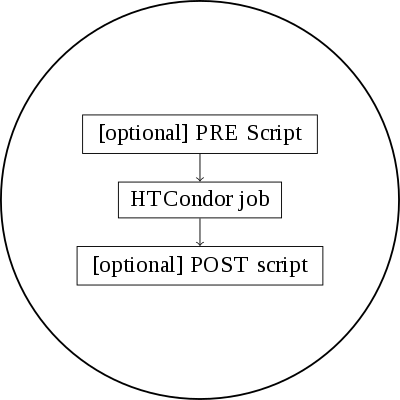
\includegraphics{user-man/dagman-node.eps}
\caption{\label{fig:dagman-node}One Node within a DAG}
\end{figure}

More than one HTCondor job may belong to a single node.
All HTCondor jobs within a node must be within
a single cluster, as given by the job ClassAd attribute \Attr{ClusterId}.
%In addition,
%all jobs within the single cluster must use the same log file.
%Separate nodes within a DAG may use different log files.

\emph{DAGMan enforces the dependencies within a DAG
using the events recorded in a separate
file that is specified by the default configuration.
If the exact same DAG were to be submitted more than once,
such that these DAGs were running at the same time,
expected them to fail in unpredictable and unexpected ways.
They would all be using the same single file to enforce dependencies. }

As DAGMan schedules and submits jobs within nodes to HTCondor,
these jobs are defined to succeed or fail based on their
return values.
This success or failure is propagated in well-defined ways to the level of
a node within a DAG.
Further progression of computation
(towards completing the DAG)
is based upon the success or failure of nodes.

The failure of a single job within a cluster
of multiple jobs
(within a single node)
causes the entire cluster of jobs to fail.
Any other jobs within the failed cluster of jobs are
immediately removed.
Each node within a DAG may be further constrained  to succeed or fail
based upon the return values of a PRE script and/or a POST script.

%%%%%%%%%%%%%%%%%%%%%%%%%%%%%%%%%%%%%%%
\subsection{The DAG Input File: Basic Commands}
%%%%%%%%%%%%%%%%%%%%%%%%%%%%%%%%%%%%%%%
\index{DAGMan!DAG input file}

The input file used by DAGMan is called a DAG input file.
It specifies the nodes of the DAG as well as the dependencies
that order the DAG.
All items are optional, except that there must be at least one \Arg{JOB}
item.

Comments may be placed in the DAG input file.
The pound character (\verb@#@) as the first character on a
line identifies the line as a comment.
Comments do not span lines.

A simple diamond-shaped DAG, as shown in
Figure~\ref{fig:dagman-diamond}
is presented as a starting point for examples.
This DAG contains 4 nodes.

\begin{figure}[hbt]
\centering
\includegraphics{user-man/dagman-diamond.eps}
\caption{\label{fig:dagman-diamond}Diamond DAG}
\end{figure}


A very simple DAG input file for this diamond-shaped DAG is

\footnotesize
\begin{verbatim}
    # File name: diamond.dag
    #
    JOB  A  A.condor 
    JOB  B  B.condor 
    JOB  C  C.condor	
    JOB  D  D.condor
    PARENT A CHILD B C
    PARENT B C CHILD D
\end{verbatim}
\normalsize

A set of basic commands appearing in a DAG input file is described below.


%%%%%%%%%%%%%%%%%%%%%%%%%%%%%%%%%%%%%%%
\subsubsection{\label{sec:dagman_job_command}JOB}
\label{dagman:JOB}
\index{DAG input file!JOB command}

The \Arg{JOB} command specifies an HTCondor job.
The syntax used for each \Arg{JOB} command is

\Opt{JOB} \Arg{JobName} \Arg{SubmitDescriptionFileName}
\oOptArg{DIR}{directory} \oOpt{NOOP} \oOpt{DONE}

A \Arg{JOB} entry maps a \Arg{JobName} to an HTCondor submit description file.
The \Arg{JobName} uniquely identifies nodes within the
DAG input file and in output messages.
Each node name, given by \Arg{JobName}, within the DAG must be unique.
The \Arg{JOB} entry must appear within the DAG input file before
other items that reference the node.

The keywords \Arg{JOB}, \Arg{DIR}, \Arg{NOOP}, and \Arg{DONE}
are not case sensitive.
Therefore, \Arg{DONE}, \Arg{Done}, and \Arg{done} are all equivalent.
The values defined for \Arg{JobName} and \Arg{SubmitDescriptionFileName}
are case sensitive, as file names 
in a file system are case sensitive.
The \Arg{JobName} can be any string that contains no white space, except
for the strings \Arg{PARENT} and \Arg{CHILD} (in upper, lower, or mixed
case).

Note that \Arg{DIR}, \Arg{NOOP}, and \Arg{DONE}, if used, must appear
in the order shown above.

The optional \Arg{DIR} keyword specifies a working directory
for this node,
from which the HTCondor job will be submitted,
and from which a \Arg{PRE} and/or
\Arg{POST} script will be run.
If a relative directory is specified, it is relative to the current working 
directory as the DAG is submitted.
Note that a DAG containing \Arg{DIR} specifications cannot
be run in conjunction with the \Arg{-usedagdir} command-line
argument to \Condor{submit\_dag}.
A "full" rescue DAG generated by a DAG run with the \Arg{-usedagdir} argument
will contain DIR specifications, so such a rescue DAG must be run
\emph{without} the \Arg{-usedagdir} argument.  (Note that "full"
rescue DAGs are no longer the default.)

\label{dagman:NOOP}
The optional \Arg{NOOP} keyword identifies that the HTCondor job within
the node is not to be submitted to HTCondor.
This optimization is useful in cases such as debugging a complex DAG structure,
where some of the individual jobs are long-running.
For this debugging of structure,
some jobs are marked as \Arg{NOOP}s, and
the DAG is initially run to verify that the control flow through
the DAG is correct.
The \Arg{NOOP} keywords are then removed before submitting the DAG.
Any PRE and POST scripts
for jobs specified with \Arg{NOOP} \emph{are} executed;
to avoid running the PRE and POST scripts, comment them out.
The job that is not submitted to HTCondor is given a return value that indicates
success, such that the node may also succeed.
Return values of any 
PRE and POST scripts may still cause the node to fail.
Even though the job specified with \Arg{NOOP} is not submitted,
its submit description file must exist;
the log file for the job is used, 
because DAGMan generates dummy submission and termination events for the job.

The optional \Arg{DONE} keyword identifies a node as being already
completed.
This is mainly used by Rescue DAGs generated by DAGMan itself,
in the event of a failure to complete the workflow.
Nodes with the \Arg{DONE} keyword are not executed when the Rescue DAG is run,
allowing the workflow to pick up from the previous endpoint.  Users
should generally not use the \Arg{DONE} keyword.
The \Arg{NOOP} keyword is more flexible in avoiding
the execution of a job within a node.
Note that, for any node marked \Arg{DONE} in a DAG, all of
its parents must also be marked \Arg{DONE}; 
otherwise, a fatal error will result.
The \Arg{DONE} keyword applies to the entire node.
A node marked with \Arg{DONE} will not have a PRE or POST script run,
and the HTCondor job will not be submitted.

%%%%%%%%%%%%%%%%%%%%%%%%%%%%%%%%%%%%%%%
\subsubsection{\label{sec:dagman_data_command}DATA}
\label{dagman:DATA}
\index{DAG input file!DATA command}

As of version 8.3.5, \Condor{dagman} no longer supports DATA nodes.

%%%%%%%%%%%%%%%%%%%%%%%%%%%%%%%%%%%%%%%
\subsubsection{\label{sec:dagman_parent_child_command}PARENT \Dots CHILD}
\label{dagman:ParentChild}
\index{DAG input file!PARENT \Dots CHILD command}

The \Arg{PARENT} \Arg{CHILD} command specifies the
dependencies within the DAG.
\index{DAGMan!describing dependencies}
Nodes are parents and/or children within the DAG.
A parent node must be completed successfully before
any of its children may be started.
A child node may only be started once
all its parents have successfully completed.

The syntax used for each dependency (PARENT/CHILD) command is

\Opt{PARENT} \Arg{ParentJobName\Dots} \Opt{CHILD} \Arg{ChildJobName\Dots}

The \Arg{PARENT} keyword is followed by one or more
\Arg{ParentJobName}s.
The \Arg{CHILD} keyword is followed by one or more
\Arg{ChildJobName}s.
Each child job depends on every parent job within the line.
A single line in the input file can specify the dependencies from one or more
parents to one or more children.
The diamond-shaped DAG example may specify the dependencies with
\begin{verbatim}
PARENT A CHILD B C
PARENT B C CHILD D
\end{verbatim}
An alternative specification for the diamond-shaped DAG
may specify some or all of the dependencies on separate lines:
\begin{verbatim}
PARENT A CHILD B C
PARENT B CHILD D
PARENT C CHILD D
\end{verbatim}

As a further example, the line
\begin{verbatim}
PARENT p1 p2 CHILD c1 c2
\end{verbatim}
produces four dependencies:
\begin{enumerate}
\item{\verb@p1@ to \verb@c1@}
\item{\verb@p1@ to \verb@c2@}
\item{\verb@p2@ to \verb@c1@}
\item{\verb@p2@ to \verb@c2@}
\end{enumerate}

%%%%%%%%%%%%%%%%%%%%%%%%%%%%%%%%%%%%%%%
\subsubsection{\label{sec:dagman_script_command}SCRIPT}
\label{dagman:SCRIPT}
\index{DAG input file!SCRIPT command}
\index{DAGMan!PRE and POST scripts}

The optional \Arg{SCRIPT} command specifies
processing that is done either before a job within
a node is submitted
or after a job within a node completes its execution.
\index{DAGMan!PRE script}
Processing done before a job is submitted is
called a \Arg{PRE} script.
Processing done after a job completes its execution is
\index{DAGMan!POST script}
called a \Arg{POST} script.
Note that the executable specified does not necessarily
have to be a shell script (Unix) or batch file (Windows);
but it should be relatively light weight because it will
be run directly on the submit machine, not submitted as
an HTCondor job.

The syntax used for each \Arg{PRE} or \Arg{POST} command is

\Opt{SCRIPT} \oOptArg{DEFER}{status time}
\Opt{PRE} \Arg{JobName}|\Opt{ALL\_NODES} \Arg{ExecutableName}
\oArg{arguments}

\Opt{SCRIPT} \oOptArg{DEFER}{status time}
\Opt{POST}  \Arg{JobName}|\Opt{ALL\_NODES} \Arg{ExecutableName}
\oArg{arguments}

The \Arg{SCRIPT} command uses
the \Arg{PRE} or \Arg{POST} keyword,
which specifies the relative timing of when the script is to be run.
The \Arg{JobName} identifies the node to which the script is attached.
The \Arg{ExecutableName}
specifies the executable (e.g., shell script or batch file) to be executed, 
and may not contain spaces.
The optional \Arg{arguments} are command line arguments to the script,
and spaces delimit the arguments.
Both \Arg{ExecutableName} and optional \Arg{arguments} are
case sensitive.

Scripts are executed on the submit machine;
the submit machine is not necessarily
the same machine upon which the node's job is run.
Further, a single cluster of HTCondor jobs may be
spread across several machines.

The optional \Arg{DEFER} feature causes a retry of only the script,
if the execution of the script exits with the
exit code given by \Arg{status}.
The retry occurs after at least \Arg{time} seconds, 
rather than being considered failed.  
While waiting for the retry,
the script does not count against a \Arg{maxpre} or \Arg{maxpost} limit.
The ordering of the \Arg{DEFER} feature within the \Arg{SCRIPT} 
specification is fixed.
It must come directly after the \Arg{SCRIPT} keyword;
this is done to avoid backward compatibility issues for any
DAG with a \Arg{JobName} of DEFER.

A PRE script is commonly used
to place files in a staging area for the jobs to use.
A POST script is commonly used
to clean up or remove files once jobs are finished running.
An example uses PRE and POST scripts to stage files
that are stored on tape.
The PRE script reads compressed input files from the tape drive,
uncompresses them, and places the resulting files in the current directory.
The HTCondor jobs can then use these files,
producing output files.
The POST script compresses the output files, writes them out to
the tape, and then removes both the staged files and the output files.

If the PRE script fails, 
then the HTCondor job associated with the node is not submitted,
and (as of version 8.5.4) the POST
script is not run either (by default).
However, if the job is submitted, and there is a POST script, the POST
script is always run once the job finishes.
(The behavior when the PRE script fails may
may be changed to run the POST script
by setting configuration variable \MacroNI{DAGMAN\_ALWAYS\_RUN\_POST} 
to \Expr{True} or by passing the \Opt{-AlwaysRunPost}
argument to \Condor{submit\_dag}.)

Progress towards completion of the DAG is based upon
the success of the nodes within the DAG.
The success of a node is based upon the success of 
the job(s), PRE script, and POST script.
A job, PRE script, or POST script with an exit value not equal to 0 is
considered failed.  
\Bold{The exit value of whatever component of the node was run last
determines the success or failure of the node.}
Table~\ref{NodeS-F} lists the definition of node success and
failure for all variations of script and job success and failure,
when \MacroNI{DAGMAN\_ALWAYS\_RUN\_POST} is set to \Expr{False}.
In this table, a dash (\Expr{-}) represents the case where a script
does not exist for the DAG, \Bold{S} represents success, 
and  \Bold{F} represents failure.

Table~\ref{NodeS-F-ARP} lists the definition of node success and
failure only for the cases where the PRE script fails,
when \MacroNI{DAGMAN\_ALWAYS\_RUN\_POST} is set to \Expr{True}.

%An exit value not equal to 0 indicates program failure,
%except as indicated by the \Arg{PRE\_SKIP} command:
%if a PRE script exits with the PRE\_SKIP value, 
%then the node succeeds and the job and the POST script are both skipped.  
%It is therefore important that a
%successful program return the exit value 0. 
%It is good practice to always
%explicitly specify a return value in the PRE script,
%returning 0 in the case of success.
%Otherwise,
%the return code of the last completed process is returned,
%which can lead to unexpected results. 

\begin{center}
\begin{table}[hbt]
\begin{tabular}{|c|c|c|c|} \hline
PRE  & JOB & POST & \Bold{Node}  \\
\hline
-  & S & - & \Bold{S}  \\
-  & F & - & \Bold{F}  \\
-  & S & S & \Bold{S}  \\
-  & S & F & \Bold{F}  \\
-  & F & S & \Bold{S}  \\
-  & F & F & \Bold{F}  \\
S  & S & - & \Bold{S}  \\
S  & F & - & \Bold{F}  \\
S  & S & S & \Bold{S}  \\
S  & S & F & \Bold{F}  \\
S  & F & S & \Bold{S}  \\
S  & F & F & \Bold{F}  \\
F  & not run & - & \Bold{F}  \\
F  & not run & not run & \Bold{F}  \\
\end{tabular}
\caption{\label{NodeS-F}Node success or failure definition with \Expr{DAGMAN\_ALWAYS\_RUN\_POST = False (the default)} }
\end{table}
\end{center}

\begin{center}
\begin{table}[hbt]
\begin{tabular}{|c|c|c|c|} \hline
PRE  & JOB & POST & \Bold{Node}  \\
F  & not run & - & \Bold{F}  \\
F  & not run & S & \Bold{S}  \\
F  & not run & F & \Bold{F}  \\
\hline
\end{tabular}
\caption{\label{NodeS-F-ARP}Node \Bold{S}uccess or \Bold{F}ailure definition with \Expr{ DAGMAN\_ALWAYS\_RUN\_POST = True} }
\end{table}
\end{center}

\Bold{Special script argument macros}

The five macros \Expr{\$JOB}, \Expr{\$RETRY}, \Expr{\$MAX\_RETRIES}, 
\Expr{\$DAG\_STATUS} and \Expr{\$FAILED\_COUNT} can be used within the
DAG input file as arguments passed to a PRE or POST script. 
The three macros \Expr{\$JOBID}, \Expr{\$RETURN}, 
and \Expr{\$PRE\_SCRIPT\_RETURN} can
be used as arguments to POST scripts.
The use of these variables is limited to being used
as an individual command
line \Arg{argument} to the script,
surrounded by spaces, in order to cause the substitution of the
variable's value.

The special macros are as follows:

\begin{itemize}
\item \index{DAGMan!JOB@\verb^$JOB^ value}
\Expr{\$JOB} evaluates to the (case sensitive) string
defined for \Arg{JobName}.

\item \index{DAGMan!RETRY@\verb^$RETRY^ value}
\Expr{\$RETRY} evaluates to an 
integer value set to 0 the first time a node is run,
and is incremented each time the node is retried. 
See section~\ref{dagman:retry} for the description of how to cause
nodes to be retried. 

\item \index{DAGMan!MAX_RETRIES@\verb^$MAX_RETRIES^ value}
\Expr{\$MAX\_RETRIES} evaluates to an integer value set 
to the maximum number of retries for the node.
See section~\ref{dagman:retry} for the description of how to cause
nodes to be retried.  
If no retries are set for the node,
\Expr{\$MAX\_RETRIES} will be set to 0.

\item \index{DAGMan!JOBID@\verb^$JOBID^ value}
\index{job ID!defined for a DAGMan node job}
\index{job!job ID!defined for a DAGMan node job}
\Expr{\$JOBID} (for POST scripts only)
evaluates to a representation of the HTCondor job ID of the node job.
It is the value of the job ClassAd attribute \Attr{ClusterId},
followed by a period,
and then followed by the value of the job ClassAd attribute \Attr{ProcId}.
An example of a job ID might be 1234.0.
For nodes with multiple jobs in the same cluster,
the \Attr{ProcId} value is the one of the last job within the cluster.

\item \index{DAGMan!return@\verb^$RETURN^ value}
\Expr{\$RETURN} (for POST scripts only) variable evaluates to
the return value of the 
HTCondor job, if there is a single job within a cluster.
With multiple jobs within the same cluster,
there are two cases to consider.
In the first case, all jobs within the cluster are successful;
the value of \Expr{\$RETURN} will be 0, indicating success.
In the second case,
one or more jobs from the cluster fail.
When \Condor{dagman} sees the first terminated event for a job that failed,
it assigns that job's return value as the value of \Expr{\$RETURN},
and it attempts to remove all remaining jobs within the cluster.
Therefore, if multiple jobs in the cluster fail with different exit codes,
a race condition determines which exit code gets assigned to \Expr{\$RETURN}.

A job that dies due to a signal is reported with a \Expr{\$RETURN} value
representing the additive inverse of the signal number.
For example, SIGKILL (signal 9) is reported as -9.
A job whose batch system submission fails is reported as -1001.
A job that is externally removed from the batch system queue
(by something other than \Condor{dagman}) is reported as -1002.

\item \index{DAGMan!PRE_SCRIPT_RETURN@\verb^$PRE_SCRIPT_RETURN^ value}
\Expr{\$PRE\_SCRIPT\_RETURN} (for POST scripts only)
variable evaluates to the return value of the PRE script of a node, 
if there is one.
If there is no PRE script, this value will be -1.
If the node job was skipped because of failure of the PRE script,
the value of \Expr{\$RETURN} will be -1004
and the value of \Expr{\$PRE\_SCRIPT\_RETURN} will be the exit value
of the PRE script;
the POST script can use this to see if the PRE script exited
with an error condition, and assign success or failure to the node, as
appropriate.

%\item \Expr{\$DAG\_STATUS} and \Expr{\$FAILED\_COUNT} are documented in
%section ~\ref{sec:DAGFinalNode} below.
%\begin{itemize}
\index{DAGMan!DAG_STATUS@\verb^$DAG_STATUS^ value}
\item \Env{\$DAG\_STATUS} is the status of the DAG.
Note that this macro's value and definition is unrelated to the attribute 
named \Attr{DagStatus} as defined for use in a node status file.
This macro's value is the same as the job ClassAd attribute \Attr{DAG\_Status}
that is defined within the \Condor{dagman} job's ClassAd.
This macro may have the following values:
\begin{itemize}
\item 0: OK
\item 1: error; an error condition different than those listed here
\item 2: one or more nodes in the DAG have failed
\item 3: the DAG has been aborted by an ABORT-DAG-ON specification
\item 4: removed; the DAG has been removed by \Condor{rm}
\item 5: cycle; a cycle was found in the DAG
\item 6: halted; the DAG has been halted (see section ~\ref{sec:DagSuspend})
\end{itemize}

\index{DAGMan!FAILED_COUNT@\verb^$FAILED_COUNT^ value}
\item \Env{\$FAILED\_COUNT} is defined by the number of nodes that have failed in the
DAG.

\end{itemize}


\Bold{Examples that use PRE or POST scripts}

Examples use the diamond-shaped DAG.
A first example uses a PRE script to expand a compressed file 
needed as input to each of the HTCondor jobs of nodes B and C.
The DAG input file:

\footnotesize
\begin{verbatim}
    # File name: diamond.dag
    #
    JOB  A  A.condor 
    JOB  B  B.condor 
    JOB  C  C.condor	
    JOB  D  D.condor
    SCRIPT PRE  B  pre.csh $JOB .gz
    SCRIPT PRE  C  pre.csh $JOB .gz
    PARENT A CHILD B C
    PARENT B C CHILD D
\end{verbatim}
\normalsize

The script \File{pre.csh} uses its command line arguments to form the file name
of the compressed file.
The script contains

\begin{verbatim}
  #!/bin/csh
  gunzip $argv[1]$argv[2]
\end{verbatim}

Therefore, the PRE script invokes  
\begin{verbatim}
  gunzip B.gz
\end{verbatim}
for node B, which uncompresses file \File{B.gz},
placing the result in file \File{B}.

A second example uses the \Expr{\$RETURN} macro.
The DAG input file contains the POST script specification:
\begin{verbatim}
  SCRIPT POST A stage-out job_status $RETURN 
\end{verbatim}
If the HTCondor job of node A exits with the value -1,
the POST script is invoked as
\begin{verbatim}
  stage-out job_status -1
\end{verbatim}

The slightly different example POST script specification
in the DAG input file
\begin{verbatim}
  SCRIPT POST A stage-out job_status=$RETURN 
\end{verbatim}
invokes the POST script with
\begin{verbatim}
  stage-out job_status=$RETURN
\end{verbatim}

This example shows that when
there is no space between the \Expr{=} sign and the variable \Expr{\$RETURN},
there is no substitution of the macro's value.

%%%%%%%%%%%%%%%%%%%%%%%%%%%%%%%%%%%%%%%
\subsubsection{\label{sec:dagman_pre_skip_command}PRE\_SKIP}
\label{dagman:PRE-SKIP}
\index{DAG input file!PRE\_SKIP command}
\index{DAGMan!skipping node execution}

The behavior of DAGMan with respect to node success or failure can
be changed with the addition of a \Arg{PRE\_SKIP} command. 
A \Arg{PRE\_SKIP} line within the DAG input file uses the syntax: 

\Opt{PRE\_SKIP} \Arg{JobName}|\Opt{ALL\_NODES} \Arg{non-zero-exit-code}

The PRE script of a node identified by \Arg{JobName} that exits with the value 
given by \Arg{non-zero-exit-code}
skips the remainder of the node entirely.  
Neither the job associated with the node nor
the POST script will be executed,
and the node will be marked as successful.

% $ % this comment just has a dollar sign so that emacs will not think
%	  we're inside of a math section and will draw things more nicely

%%%%%%%%%%%%%%%%%%%%%%%%%%%%%%%%%%%%%%%
\subsection{\label{sec:DAG-command_order}Command Order}
\label{dagman:command order}
\index{DAG input file!command order}
\index{DAGMan!command order}

As of version 8.5.6, commands referencing a \Arg{JobName} \emph{can}
come before the JOB command defining that \Arg{JobName}.

For example, the command sequence
\begin{verbatim}
SCRIPT PRE NodeA foo.pl
VARS NodeA state="Wisconsin"
JOB NodeA bar.sub
\end{verbatim}
is now legal (it would have been illegal in 8.5.5 and all previous
versions).

%%%%%%%%%%%%%%%%%%%%%%%%%%%%%%%%%%%%%%%
\subsection{Node Job Submit File Contents}
%%%%%%%%%%%%%%%%%%%%%%%%%%%%%%%%%%%%%%%
\index{DAGMan!node job submit description file}

Each node in a DAG may use a unique submit description file.
A key limitation is that
each HTCondor submit description file must submit jobs
described by a single cluster number;
DAGMan cannot deal with a submit description file producing
multiple job clusters.

Consider again the diamond-shaped DAG example, 
where each node job uses the same submit description file.

\begin{verbatim}
    # File name: diamond.dag
    #
    JOB  A  diamond_job.condor 
    JOB  B  diamond_job.condor 
    JOB  C  diamond_job.condor	
    JOB  D  diamond_job.condor
    PARENT A CHILD B C
    PARENT B C CHILD D
\end{verbatim}

Here is a sample HTCondor submit description file
for this DAG:

\index{DAGMan!example submit description file}
\begin{verbatim}
    # File name: diamond_job.condor
    #
    executable   = /path/diamond.exe
    output       = diamond.out.$(cluster)
    error        = diamond.err.$(cluster)
    log          = diamond_condor.log
    universe     = vanilla
    queue
\end{verbatim}

Since each node uses the same HTCondor submit description file,
this implies that each node within the DAG runs the
same job.
The \MacroUNI{Cluster} macro
produces unique file names for each job's output.

\index{ClassAd job attribute!DAGParentNodeNames}
\index{DAGParentNodeNames!job ClassAd attribute}
The job ClassAd attribute \Attr{DAGParentNodeNames} is also available
for use within the submit description file. 
It defines a comma separated list of each \Arg{JobName}
which is a parent node of this job's node.
This attribute may be used in the \SubmitCmd{arguments} command
for all but scheduler universe jobs.
For example, if the job has two parents, with \Arg{JobName}s B and C,
the submit description file command
\begin{verbatim}
arguments = $$([DAGParentNodeNames])
\end{verbatim}
will pass the string \AdStr{B,C} as the command line argument when invoking
the job.

%%%%%%%%%%%%%%%%%%%%%%%%%%%%%%%%%%%%%%%
\subsection{\label{dagman:submitdag}DAG Submission}
%%%%%%%%%%%%%%%%%%%%%%%%%%%%%%%%%%%%%%%
\index{DAGMan!DAG submission}

A DAG is submitted using the tool \Condor{submit\_dag}.
The manual
page~\pageref{man-condor-submit-dag}
details the command.
The simplest of DAG submissions has the syntax

\Condor{submit\_dag} \Arg{DAGInputFileName}

and the current working directory contains the DAG input file.

The diamond-shaped DAG example may be submitted with

\begin{verbatim}
condor_submit_dag diamond.dag
\end{verbatim}

Do not submit the same DAG, with same DAG input file, 
from within the same directory, 
such that more than one of this same DAG is running at the same time.
It will fail in an unpredictable manner,
as each instance of this same DAG will attempt to use the same
file to enforce dependencies.
 
To increase robustness and guarantee recoverability, the 
\Condor{dagman} process is run as an HTCondor job.
As such, it needs a submit description file.
\Condor{submit\_dag} generates this needed submit description file,
naming it by appending \File{.condor.sub} to the name of the DAG input file.
This submit description file may be edited if the DAG is submitted with

\begin{verbatim}
condor_submit_dag -no_submit diamond.dag
\end{verbatim}
causing \Condor{submit\_dag} to create the submit description file,
but not submit \Condor{dagman} to HTCondor.
To submit the DAG, once the submit description file is edited,
use

\begin{verbatim}
condor_submit diamond.dag.condor.sub
\end{verbatim}

Submit machines with limited resources are supported by
command line options that place limits on the submission and handling 
of HTCondor jobs and PRE and POST scripts. 
Presented here are descriptions of the command line options
to \Condor{submit\_dag}.
These same limits can be set in configuration.
Each limit is applied within a single DAG.

%%%%%%%%%%%%%%%%%%%%%%%%%%%%%%%%%%%%%%%
\subsubsection{\label{sec:DAG-throttling}DAG Throttling}
\index{DAGMan!throttling}

\Bold{Total nodes/clusters:}
The \Opt{-maxjobs} option 
specifies the maximum number of clusters that \Condor{dagman}
can submit at one time.
Since each node corresponds to a single cluster,
this limit restricts the number of nodes that can be submitted (in the
HTCondor queue) at a time.
It is commonly used when
there is a limited amount of input file staging capacity.
As a specific example, consider a case where each node represents
a single HTCondor proc that requires 4 MB of input files,
and the proc will run in a directory with a volume of 100 MB
of free space.
Using the argument \Opt{-maxjobs 25} guarantees that a maximum
of 25 clusters, using a maximum of 100 MB of space,
will be submitted to HTCondor at one time.
(See the \Condor{submit\_dag} man page (~\ref{man-condor-submit-dag})
for more information.  Also see the equivalent
\Macro{DAGMAN\_MAX\_JOBS\_SUBMITTED} configuration option
(~\ref{param:DAGManMaxJobsSubmitted}).)

\Bold{Idle procs:}
The number of idle procs within a given DAG can be limited with
the optional command line argument \Opt{-maxidle}. 
\Condor{dagman} will not submit any more node jobs 
until the number of idle procs in the DAG goes below this
specified value,
even if there are ready nodes in the DAG.
This allows \Condor{dagman} to submit jobs in a way that adapts to
the load on the HTCondor pool at any given time.  If the pool is
lightly loaded, \Condor{dagman} will end up submitting more jobs;
if the pool is heavily loaded, \Condor{dagman} will submit fewer jobs.
(See the \Condor{submit\_dag} man page (~\ref{man-condor-submit-dag})
for more information.  Also see the equivalent
\Macro{DAGMAN\_MAX\_JOBS\_IDLE} configuration option
(~\ref{param:DAGManMaxJobsIdle}).)

Note that the \Opt{-maxjobs} option applies to counts of
\emph{clusters}, whereas the \Opt{-maxidle} option
applies to counts of \emph{procs}.  Unfortunately, this can
be a bit confusing.  Of course, if none of your submit files
create more than one proc, the distinction doesn't matter.
For example, though, a node job submit file that queues
5 procs will count as one for \Opt{-maxjobs}, but five
for \Opt{-maxidle} (if all of the procs are idle).

\Bold{Subsets of nodes:}
Node submission can also be throttled in a finer-grained manner by
grouping nodes into categories.  See section ~\ref{sec:DAG-node-category}
for more details.

\Bold{PRE/POST scripts:}
Since PRE and POST scripts run on the submit machine,
it may be desirable to limit the number of PRE or POST scripts running
at one time.
The optional \Opt{-maxpre} command line argument limits the number of PRE
scripts that may be running at one time,
and the optional \Opt{-maxpost} command line argument limits the number
of POST scripts that may be running at one time.
(See the \Condor{submit\_dag} man page (~\ref{man-condor-submit-dag})
for more information.  Also see the equivalent
\Macro{DAGMAN\_MAX\_PRE\_SCRIPTS} (~\ref{param:DAGManMaxPreScripts}) and
\Macro{DAGMAN\_MAX\_POST\_SCRIPTS} (~\ref{param:DAGManMaxPostScripts})
configuration options.)

%%%%%%%%%%%%%%%%%%%%%%%%%%%%%%%%%%%%%%%
\subsection{\label{sec:DAGPaths}File Paths in DAGs}
%%%%%%%%%%%%%%%%%%%%%%%%%%%%%%%%%%%%%%%
\index{DAGMan!file paths in DAGs}

\Condor{dagman} assumes that all relative paths in a
DAG input file and the associated HTCondor submit description files
are relative to the current
working directory when \Condor{submit\_dag} is run.  
This works well for submitting a single DAG.
It presents problems when multiple independent DAGs are submitted
with a single invocation of \Condor{submit\_dag}.
Each of these independent DAGs would logically be in its own directory, 
such that it could be run or tested independent of other DAGs.
Thus, all references to files will be designed to be relative to
the DAG's own directory.

%Note that 
%relative paths in submit description files can be modified by the submit command
%\SubmitCmd{initialdir}; 
%see the \Condor{submit} manual page at ~\ref{man-condor-submit} 
%for more details on this command.
%The remainder of this discussion ignores \SubmitCmd{initialdir}.

Consider an example DAG within a directory named \File{dag1}.
There would be a DAG input file, named \File{one.dag} for this example.
Assume the contents of this DAG input file specify a node job with
\begin{verbatim}
  JOB A  A.submit
\end{verbatim}
Further assume that partial contents of submit description file 
\File{A.submit} specify
\begin{verbatim}
  executable = programA
  input      = A.input
\end{verbatim}

Directory contents are 
\begin{verbatim}
    dag1 (directory)
          one.dag
          A.submit
          programA
          A.input
\end{verbatim}

All file paths are correct relative to the \File{dag1} directory.
Submission of this example DAG sets the current working directory
to \File{dag1} and invokes \Condor{submit\_dag}:
\begin{verbatim}
  cd dag1
  condor_submit_dag one.dag
\end{verbatim}

Expand this example such that there are now two independent DAGs,
and each is contained within its own directory. 
For simplicity, assume that the DAG in \File{dag2} has remarkably
similar files and file naming as the DAG in \File{dag1}.
Assume that the directory contents are 
\begin{verbatim}
    parent (directory)
         dag1 (directory)
               one.dag
               A.submit
               programA
               A.input
         dag2 (directory)
               two.dag
               B.submit
               programB
               B.input
\end{verbatim}

The goal is to use a single invocation of \Condor{submit\_dag}
to run both dag1 and dag2.
The invocation
\begin{verbatim}
  cd parent
  condor_submit_dag dag1/one.dag dag2/two.dag
\end{verbatim}
\emph{does not work}.
Path names are now relative to \File{parent}, 
which is \emph{not} the desired behavior.

The solution is 
the \Arg{-usedagdir} command line argument to \Condor{submit\_dag}.
This feature runs each DAG as if \Condor{submit\_dag} had been run 
in the directory in which the relevant DAG file exists.
A working invocation is
\begin{verbatim}
  cd parent
  condor_submit_dag -usedagdir dag1/one.dag dag2/two.dag
\end{verbatim}

Output files will be placed in the correct directory, and
the \File{.dagman.out} file will also be in the correct directory.
A Rescue DAG file will be written to
the current working directory, which is the directory when
\Condor{submit\_dag} is invoked.
The Rescue DAG should be run from that same current working directory.
The Rescue DAG includes all the path information necessary to
run each node job in the proper directory.

%If all paths in the DAG input file(s) and the relevant submit
%description files are absolute,
%the \Arg{-usedagdir} argument is not needed;
%however, using absolute paths is NOT generally a good idea.

%For a DAG that \emph{does not} use \Arg{-usedagdir}, 
%relative paths can still work for multiple DAGs, 
%if all file paths are given relative to
%the current working directory as \Condor{submit\_dag} is executed.
%This implies that DAGs in separate directories
%cannot be submitted from their own directories;
%submission only works from the parent directory the paths are set up for.

Use of \Arg{-usedagdir} does \emph{not} work in conjunction with
a JOB node specification within the DAG input file using
the \Arg{DIR} keyword.
Using both will be detected and generate an error. 

%%%%%%%%%%%%%%%%%%%%%%%%%%%%%%%%%%%%%%%
\subsection{\label{sec:DAGMonitoring}DAG Monitoring and DAG Removal}
%%%%%%%%%%%%%%%%%%%%%%%%%%%%%%%%%%%%%%%
\index{DAGMan!DAG monitoring}
\index{DAGMan!DAG removal}

%TEMP -- this section needs lots of improvement... (dagman.out, node
% status file, jobstate.log file, halt file, etc.)

After submission, the progress of the DAG can be monitored
by looking at the job event log file(s),
observing the e-mail that job submission to HTCondor causes,
or by using \Condor{q} \Arg{-dag}.

There is also a large amount of information logged in an extra file.
The name of this extra file is produced by appending
\File{.dagman.out} to the name of the DAG input file; 
for example, if the DAG input file is \File{diamond.dag}, 
this extra file is named \File {diamond.dag.dagman.out}.
If this extra file grows too large, limit its size
with the configuration variable \Macro{MAX\_DAGMAN\_LOG},
as defined in section~\ref{param:MaxSubsysLog}.
The \File{dagman.out} file is an important resource for
debugging; save this file if a problem occurs. 
The \File{dagman.out} is appended to, rather than overwritten, 
with each new DAGMan run.

To remove an entire DAG, consisting of the \Condor{dagman} job, 
plus any jobs submitted to HTCondor,
remove the \Condor{dagman} job by running \Condor{rm}.
For example,
%TEMP -- example needs to be changed to match current condor_q
\footnotesize
\begin{verbatim}
% condor_q
-- Submitter: turunmaa.cs.wisc.edu : <128.105.175.125:36165> : turunmaa.cs.wisc.edu
 ID      OWNER          SUBMITTED     RUN_TIME ST PRI SIZE CMD
  9.0   taylor         10/12 11:47   0+00:01:32 R  0   8.7  condor_dagman -f -
 11.0   taylor         10/12 11:48   0+00:00:00 I  0   3.6  B.out
 12.0   taylor         10/12 11:48   0+00:00:00 I  0   3.6  C.out

    3 jobs; 2 idle, 1 running, 0 held

% condor_rm 9.0
\end{verbatim}
\normalsize

When a \Condor{dagman} job is removed, all node jobs (including sub-DAGs)
of that \Condor{dagman} will be removed by the \Condor{schedd}.  As of version
8.5.8, the default is that \Condor{dagman} itself also removes the
node jobs (to fix a race condition that could result in "orphaned"
node jobs).  (The \Condor{schedd} has to remove the node jobs to deal with
the case of removing a \Condor{dagman} job that has been held.)

The previous behavior of \Condor{dagman} itself \emph{not} removing
the node jobs can be restored by setting the
\MacroNI{DAGMAN\_REMOVE\_NODE\_JOBS} configuration macro
(see ~\ref{param:DAGManRemoveNodeJobs})
to \Expr{False}.  This will decrease the load on the \Condor{schedd},
at the cost of allowing the possibility of "orphaned" node jobs.

A removed DAG will be considered failed unless the
DAG has a FINAL node that succeeds.

%TEMP -- this needs to be fixed/clarified
In the case where a
machine is scheduled to go down,
DAGMan will clean up memory and exit.
However, it will leave any submitted jobs
in the HTCondor queue.

%%%%%%%%%%%%%%%%%%%%%%%%%%%%%%%%%%%%%%%
\subsection{\label{sec:DagSuspend}Suspending a Running DAG}
%%%%%%%%%%%%%%%%%%%%%%%%%%%%%%%%%%%%%%%
\index{DAGMan!suspending a running DAG}

It may be desired to temporarily suspend a running DAG.
For example, the load may be high on the submit machine,
and therefore it is desired to prevent DAGMan from
submitting any more jobs until the load goes down.
There are two ways to suspend (and resume) a running DAG.

\begin{itemize}
\item Use \Condor{hold}/\Condor{release} on the \Condor{dagman} job.

After placing the \Condor{dagman} job on hold,
no new node jobs will be submitted,
and no PRE or POST scripts will be run.
Any node jobs already in the HTCondor queue will continue undisturbed.
Any running PRE or POST scripts will be killed.
If the \Condor{dagman} job is left on hold,
it will remain in the HTCondor queue after all of the currently running
node jobs are finished.
To resume the DAG, use \Condor{release} on the \Condor{dagman} job.

Note that while the \Condor{dagman} job is on hold,
no updates will be made to the \File{dagman.out} file.

\item Use a DAG halt file.

The second way of suspending a DAG uses the existence of a specially-named
file to change the state of the DAG.
When in this halted state,
no PRE scripts will be run, and no node jobs will be submitted.  
Running node jobs will continue undisturbed.
A halted DAG will still run POST scripts,
and it will still update the \File{dagman.out} file.
This differs from behavior of a DAG that is held.
Furthermore, a halted DAG will not remain in the queue indefinitely;
when all of the running node jobs have finished, 
DAGMan will create a Rescue DAG and exit.

To resume a halted DAG, remove the halt file.

The specially-named file must be placed in the same directory
as the DAG input file.
The naming is the same as the DAG input file concatenated with the
string \File{.halt}.
For example, if the DAG input file is \File{test1.dag}, 
then \File{test1.dag.halt} will be the required name of the halt file.

As any DAG is first submitted with \Condor{submit\_dag}, 
a check is made for a halt file.
If one exists, it is removed.
\end{itemize}

\Bold{Note that neither \Condor{hold} nor a DAG halt is propagated to
sub-DAGs.}
In other words, if you \Condor{hold} or create a halt file for a DAG that
has sub-DAGs, any sub-DAGs that are already in the queue will continue
to submit node jobs.

A \Condor{hold} or DAG halt \emph{does}, however, apply to splices,
because they are merged into the parent DAG and controlled by a single
\Condor{dagman} instance.

%%%%%%%%%%%%%%%%%%%%%%%%%%%%%%%%%%%%%%%
\subsection{\label{sec:AdvDAGMan}Advanced Features of DAGMan}
%%%%%%%%%%%%%%%%%%%%%%%%%%%%%%%%%%%%%%%


%%%%%%%%%%%%%%%%%%%%%%%%%%%%%%%%%%%%%%%
\subsubsection{\label{dagman:retry}Retrying Failed Nodes}
\index{DAG input file!RETRY command}
\index{DAGMan!retrying failed nodes}

DAGMan can retry any failed node in a DAG by
specifying the node in the DAG input file 
with the \Arg{RETRY} command.
The use of retry is optional.
The syntax for retry is

\Opt{RETRY} \Arg{JobName}|\Opt{ALL\_NODES} \Arg{NumberOfRetries}
\oOptArg{UNLESS-EXIT}{value}

where \Arg{JobName} identifies the node.
\Arg{NumberOfRetries} is an integer
number of times to retry the node after failure.
The implied number of retries for any node is 0,
the same as not having a retry line in the file. 
Retry is implemented on nodes, not parts of a node.

The diamond-shaped DAG example may be modified to
retry node C:

\footnotesize
\begin{verbatim}
    # File name: diamond.dag
    #
    JOB  A  A.condor 
    JOB  B  B.condor 
    JOB  C  C.condor	
    JOB  D  D.condor
    PARENT A CHILD B C
    PARENT B C CHILD D
    Retry  C 3
\end{verbatim}
\normalsize

If node C is marked as failed for any reason,
then it is started over as a first retry.
The node will be tried a second and third time,
if it continues to fail.
If the node is marked as successful, then further retries do not occur.

Retry of a node may be short circuited using the
optional keyword \Arg{UNLESS-EXIT}, followed by an integer exit value.
If the node exits with the specified integer exit value,
then no further processing will be done
on the node. 

The macro \Env{\$RETRY} evaluates to an 
integer value, set to 0 first time a node is run,
and is incremented each time for each time the node is retried. 
The macro \Env{\$MAX\_RETRIES} is the value set for
\Arg{NumberOfRetries}.
These macros may be used as arguments passed to a PRE or POST script.

%%%%%%%%%%%%%%%%%%%%%%%%%%%%%%%%%%%%%%%
\subsubsection{\label{dagman:abort}Stopping the Entire DAG}
\index{DAG input file!ABORT-DAG-ON command}
\index{DAGMan!aborting a DAG}

The \Arg{ABORT-DAG-ON} command provides a way
to abort the entire DAG if a given node returns a specific exit
code.  The syntax for \Arg{ABORT-DAG-ON} is

\Opt{ABORT-DAG-ON} \Arg{JobName}|\Opt{ALL\_NODES} \Arg{AbortExitValue}
\oOptArg{RETURN}{DAGReturnValue}

If the return value of the node specified by \Arg{JobName}
matches \Arg{AbortExitValue},
the DAG is immediately aborted.
A DAG abort differs from a node failure,
in that a DAG abort causes all nodes within the DAG to be stopped immediately.
This includes removing the jobs in nodes that are currently running.
A node failure differs, as it would allow the DAG to continue running,
until no more progress can be made due to dependencies.

The behavior differs based on the existence of PRE and/or POST scripts.
If a PRE script returns the \Arg{AbortExitValue} value,
the DAG is immediately aborted.
If the HTCondor job within a node returns the \Arg{AbortExitValue} value,
the DAG is aborted if the node has no POST script.
If the POST script returns the \Arg{AbortExitValue} value, the DAG is aborted.

An abort overrides node retries. 
If a node returns the abort exit value,
the DAG is aborted,
even if the node has retry specified.

When a DAG aborts, by default it exits with the node return value that
caused the abort.  This can be changed by 
using  the optional \Arg{RETURN} keyword along
with specifying the desired \Arg{DAGReturnValue}.
The DAG abort return value
can be used for DAGs within DAGs,
allowing an inner DAG to cause an abort of an outer DAG.

A DAG return value other than 0, 1, or 2 will cause the
\Condor{dagman} job to stay in the queue after it exits
and get retried, unless the \AdAttr{on\_exit\_remove} expression in the
\File{.condor.sub} file is manually modified.

Adding \Arg{ABORT-DAG-ON} for node C in the diamond-shaped
DAG
\footnotesize
\begin{verbatim}
    # File name: diamond.dag
    #
    JOB  A  A.condor 
    JOB  B  B.condor 
    JOB  C  C.condor	
    JOB  D  D.condor
    PARENT A CHILD B C
    PARENT B C CHILD D
    Retry  C 3
    ABORT-DAG-ON C 10 RETURN 1
\end{verbatim}
\normalsize

causes the DAG to be aborted, if node C exits with a return value of 10.
Any other currently running nodes, 
of which only node B is a possibility for this particular example, 
are stopped and removed.
If this abort occurs, the return value for the DAG is 1.


%%%%%%%%%%%%%%%%%%%%%%%%%%%%%%%%%%%%%%%
\subsubsection{\label{dagman:VARS}Variable Values Associated with Nodes}
\index{DAG input file!VARS command}
\index{DAGMan!VARS (macro for submit description file)}

Macros defined for DAG nodes can be used within the submit description
file of the node job. 
The \Arg{VARS} command provides a method for defining a macro.
Macros are defined on a per-node basis, using the syntax

\Opt{VARS} \Arg{JobName}|\Opt{ALL\_NODES} \Arg{macroname=}\Arg{"string"}
[\Arg{macroname=}\Arg{"string"\Dots}]

The macro may be used within the
submit description file of the relevant node.  
A \Arg{macroname} may contain alphanumeric characters (a-z, A-Z, and 0-9)
and the underscore character.
The space character delimits macros,
such that there may be more than one macro defined on a single line.
Multiple lines defining macros for the same node are permitted.

Correct syntax requires that the \Arg{string} must be
enclosed in double quotes.
To use a double quote mark within a \Arg{string},
escape the double quote mark with the backslash character (\verb@\@).
To add the backslash character itself, use two backslashes (\verb@\\@).

A restriction is that the \Arg{macroname} itself cannot begin with the string
\Expr{queue},
in any combination of upper or lower case letters.

\Bold{Examples}

If the DAG input file contains
\footnotesize
\begin{verbatim}
    # File name: diamond.dag
    #
    JOB  A  A.submit 
    JOB  B  B.submit 
    JOB  C  C.submit	
    JOB  D  D.submit
    VARS A state="Wisconsin"
    PARENT A CHILD B C
    PARENT B C CHILD D

\end{verbatim}
\normalsize

then the submit description file \File{A.submit} may use 
the macro \verb@state@.
Consider this 
submit description file \File{A.submit}:

\footnotesize
\begin{verbatim}
    # file name: A.submit
    executable = A.exe
    log        = A.log
    arguments  = "$(state)"
    queue
\end{verbatim}
\normalsize
The macro value expands to become a command-line argument in 
the invocation of the job.
The job is invoked with
\footnotesize
\begin{verbatim}
A.exe Wisconsin
\end{verbatim}
\normalsize

The use of macros may allow a reduction in the number 
of distinct submit description files.
A separate example shows this intended use of \Arg{VARS}.
In the case where the submit description file for each node
varies only in file naming, 
macros reduce the number of submit description files to one.

This example references a single submit description file for each of
the nodes in the DAG input file, 
and it uses the \Arg{VARS} entry to name files used by each job.

The relevant portion of the DAG input file appears as 
\begin{verbatim}
    JOB A theonefile.sub
    JOB B theonefile.sub
    JOB C theonefile.sub

    VARS A filename="A"
    VARS B filename="B"
    VARS C filename="C"
\end{verbatim}

The submit description file appears as 
\footnotesize
\begin{verbatim}
    # submit description file called:  theonefile.sub
    executable   = progX
    output       = $(filename)
    error        = error.$(filename)
    log          = $(filename).log
    queue
\end{verbatim}
\normalsize

For a DAG such as this one, but with thousands of nodes,
the ability to write and maintain a single submit description file 
together with a single, yet more complex, DAG input file is worthwhile.

% Note: this is an alternative to subsubsubsection, which we don't have.
\begin{description}
\item[Multiple macroname definitions]
\end{description}

If a macro name for a specific node in a DAG is defined more than once,
as it would be with the partial file contents
\begin{verbatim}
  JOB job1 job1.submit
  VARS job1 a="foo"
  VARS job1 a="bar"
\end{verbatim}
a warning is written to the log, of the format 
\begin{verbatim}
Warning: VAR <macroname> is already defined in job <JobName>
Discovered at file "<DAG input file name>", line <line number>
\end{verbatim}

The behavior of DAGMan is such that all definitions for the macro exist,
but only the last one defined is used as the variable's value.
Using this example, 
if the \File{job1.submit} submit description file contains
\begin{verbatim}
  arguments = "$(a)"
\end{verbatim}
then the argument will be \Expr{bar}.

% Note: this is an alternative to subsubsubsection, which we don't have.
\begin{description}
\item[Special characters within VARS string definitions]
\end{description}
\index{DAGMan!VARS (use of special characters)}

The value defined for a macro may contain spaces and tabs.
It is also possible to have double quote marks and
backslashes within a value.
In order to have spaces or tabs within a value specified for a command line
argument,
use the New Syntax format for the \SubmitCmdNI{arguments} submit command,
as described in section~\ref{man-condor-submit-arguments}.
Escapes for double quote marks
depend on whether the New Syntax or Old Syntax format is used
for the \SubmitCmdNI{arguments} submit command.
Note that in both syntaxes,
double quote marks require two levels of escaping:
one level is for the parsing of the DAG input file, and the other level is for
passing the resulting value through \Condor{submit}.

As of HTCondor version 8.3.7, 
single quotes are permitted within the value specification.  
For the specification of command line \SubmitCmdNI{arguments}, 
single quotes can be used in three ways:
\begin{itemize}
\item in Old Syntax, within a macro's value specification
\item in New Syntax, within a macro's value specification
\item in New Syntax only, to delimit an argument containing white space 
\end{itemize}
There are examples of all three cases below.  
In New Syntax, 
to pass a single quote as part of an argument, 
escape it with another single quote
for \Condor{submit} parsing as in the example's NodeA \Expr{fourth} macro.

As an example that shows uses of all special characters, 
here are only the relevant parts of a DAG input file.
Note that the NodeA value for the macro \Expr{second} contains a tab.
\footnotesize
\begin{verbatim}
    VARS NodeA first="Alberto Contador"
    VARS NodeA second="\"\"Andy	Schleck\"\""
    VARS NodeA third="Lance\\ Armstrong"
    VARS NodeA fourth="Vincenzo ''The Shark'' Nibali"
    VARS NodeA misc="!@#$%^&*()_-=+=[]{}?/"
    
    VARS NodeB first="Lance_Armstrong"
    VARS NodeB second="\\\"Andreas_Kloden\\\""
    VARS NodeB third="Ivan\\_Basso"
    VARS NodeB fourth="Bernard_'The_Badger'_Hinault"
    VARS NodeB misc="!@#$%^&*()_-=+=[]{}?/"

    VARS NodeC args="'Nairo Quintana' 'Chris Froome'"
\end{verbatim}
\normalsize

Consider an example in which
the submit description file for NodeA uses the New Syntax for the
\SubmitCmdNI{arguments} command:
\footnotesize
\begin{verbatim}
  arguments = "'$(first)' '$(second)' '$(third)' '($fourth)' '$(misc)'"
\end{verbatim}
\normalsize
The single quotes around each variable reference are only necessary
if the variable value may contain spaces or tabs.
The resulting values passed to the NodeA executable are:
\footnotesize
\begin{verbatim}
  Alberto Contador
  "Andy	Schleck"
  Lance\ Armstrong
  Vincenzo 'The Shark' Nibali
  !@#$%^&*()_-=+=[]{}?/
\end{verbatim}
\normalsize

Consider an example in which
the submit description file for NodeB uses the Old Syntax for the
\SubmitCmdNI{arguments} command:
\footnotesize
\begin{verbatim}
  arguments = $(first) $(second) $(third) $(fourth) $(misc)
\end{verbatim}
\normalsize

The resulting values passed to the NodeB executable are:
\footnotesize
\begin{verbatim}
  Lance_Armstrong
  "Andreas_Kloden"
  Ivan\_Basso
  Bernard_'The_Badger'_Hinault
  !@#$%^&*()_-=+=[]{}?/
\end{verbatim}
\normalsize

Consider an example in which
the submit description file for NodeC uses the New Syntax for the
\SubmitCmdNI{arguments} command:
\footnotesize
\begin{verbatim}
  arguments = "$(args)"
\end{verbatim}
\normalsize

The resulting values passed to the NodeC executable are:
\footnotesize
\begin{verbatim}
  Nairo Quintana
  Chris Froome
\end{verbatim}
\normalsize

% Note: this is an alternative to subsubsubsection, which we don't have.
\begin{description}
\item[Using special macros within a definition]
\end{description}

The \verb@$(JOB)@ and \verb@$(RETRY)@ macros may be used within a
definition of the \Arg{string} that defines a variable.
This usage requires parentheses,
such that proper macro substitution may take place when
the macro's value is only a portion of the string.
\begin{itemize}
\item \verb@$(JOB)@ expands to the node \Arg{JobName}. 
If the \Arg{VARS} line appears in a DAG file used as a splice file, 
then \verb@$(JOB)@ will be the fully scoped name of the node.

For example, the DAG input file lines
\begin{verbatim}
  JOB  NodeC NodeC.submit
  VARS NodeC nodename="$(JOB)"
\end{verbatim}
set \Expr{nodename} to \Expr{NodeC},
and the DAG input file lines
\begin{verbatim}
  JOB  NodeD NodeD.submit
  VARS NodeD outfilename="$(JOB)-output"
\end{verbatim}
set \Expr{outfilename} to \Expr{NodeD-output}.

\item \verb@$(RETRY)@ expands to 0 the first time a node is run;
the value is incremented each time the node is retried.
For example:
\begin{verbatim}
  VARS NodeE noderetry="$(RETRY)"
\end{verbatim}
\end{itemize}

% Note: this is an alternative to subsubsubsection, which we don't have.
\begin{description}
\item[Using VARS to define ClassAd attributes]
\end{description}

The \Arg{macroname} may also begin with a \Expr{+} character, in which case it
names a ClassAd attribute. For example, the VARS specification
\begin{verbatim}
  VARS NodeF +A="\"bob\""
\end{verbatim}
results in the job ClassAd attribute
\begin{verbatim}
  A = "bob"
\end{verbatim}
Note that ClassAd string values must be quoted, hence there are escaped
quotes in the example above.  The outer quotes are consumed in the parsing of
the DAG input file, so the escaped inner quotes remain in the definition
of the attribute value.

Continuing this example,
it allows the HTCondor submit description file for NodeF to use
the following line:
\begin{verbatim}
  arguments = "$$([A])"
\end{verbatim}

The special macros may also be used.
For example
\begin{verbatim}
  VARS NodeG +B="$(RETRY)"
\end{verbatim}
places the numerical attribute
\begin{verbatim}
  B = 1
\end{verbatim}
into the ClassAd when the NodeG job is run for a second time,
which is the first retry and the value 1. 

%%%%%%%%%%%%%%%%%%%%%%%%%%%%%%%%%%%%%%%
\subsubsection{\label{sec:DAG-SetNodePriority}Setting Priorities for Nodes}
\index{DAG input file!PRIORITY command}
\index{DAGMan!node priorities}

The \Arg{PRIORITY} command assigns a priority to a DAG node
(and to the HTCondor job(s) associated with the node).
The syntax for \Arg{PRIORITY} is

\Opt{PRIORITY} \Arg{JobName}|\Opt{ALL\_NODES} \Arg{PriorityValue}

The priority value is an integer (which can be negative).  A larger
numerical priority is better.  The default priority is 0.

The node priority affects the order in which nodes that are ready
(all of their parent nodes have finished successfully)
at the same time will be submitted.  The node priority also sets
the node job's priority in the queue (that is, its \Attr{JobPrio}
attribute), which affects the order in which jobs will be run once
they are submitted (see ~\ref{sec:JobPriority} for more information
about job priority).
The node priority only affects the order of job submission
\emph{within a given DAG}; but once jobs are submitted, their
\Attr{JobPrio} value affects the order in which they will be run
relative to all jobs submitted by the same user.

Sub-DAGs can have priorities, just as "regular" nodes can.  (The
priority of a sub-DAG will affect the priorities of its nodes:
see "effective node priorities" below.)
Splices cannot be assigned a priority, but individual nodes within
a splice \emph{can} be assigned priorities.

Note that node priority does \emph{not} override the DAG dependencies.
Also note that node priorities are not \emph{guarantees}
of the relative order in which nodes will be run, even among nodes that
become ready at the same time -- so node priorities
should not be used as a substitute for parent/child dependencies.
In other words, priorities should be used when it is preferable, but
not required, that some jobs run before others.  (The order in which
jobs are run once they are submitted can be affected by many things
other than the job's priority; for example, whether there are machines
available in the pool that match the job's requirements.)

PRE scripts can affect the order in which jobs run, so DAGs containing
PRE scripts may not submit the nodes in exact priority order, even if
doing so would satisfy the DAG dependencies.

Node priority is most relevant if
node submission is throttled (via the \Arg{-maxjobs} or \Arg{-maxidle}
command-line arguments or the \MacroNI{DAGMAN\_MAX\_JOBS\_SUBMITTED} or
\MacroNI{DAGMAN\_MAX\_JOBS\_IDLE} configuration variables), or if
there are not enough resources in the pool to immediately run all
submitted node jobs.  This is often the case for DAGs with
large numbers of "sibling" nodes, or DAGs running on heavily-loaded
pools.

% Note: this is an alternative to subsubsubsection, which we don't have.
\begin{description}
\item[Example]
\end{description}

Adding \Arg{PRIORITY} for node C in the diamond-shaped
DAG:
\footnotesize
\begin{verbatim}
    # File name: diamond.dag
    #
    JOB  A  A.condor 
    JOB  B  B.condor 
    JOB  C  C.condor	
    JOB  D  D.condor
    PARENT A CHILD B C
    PARENT B C CHILD D
    Retry  C 3
    PRIORITY C 1
\end{verbatim}
\normalsize

This will cause node C to be submitted (and, mostly likely, run) before
node B.
Without this priority setting for node C, node B would be submitted first
because the "JOB" statement for node B comes earlier in the DAG file
than the "JOB" statement for node C.

% Note: this is an alternative to subsubsubsection, which we don't have.
\begin{description}
\item[Effective node priorities]
\end{description}

\Bold{The "effective" priority for a node (the priority
controlling the order in which nodes are actually submitted, and which
is assigned to \Attr{JobPrio}) is the sum of the
explicit priority (specified in the DAG file) and the priority of
the DAG itself.}  DAG priorities also default to 0, so they
are most relevant for sub-DAGs (although a top-level DAG can
be submitted with a non-zero priority by specifying a \Opt{-priority}
value on the \Condor{submit\_dag} command line).
\Bold{This algorithm for
calculating effective priorities is a simplification introduced in
version 8.5.7 (a node's effective priority is no longer dependent on
the priorities of its parents).}

Here is an example to clarify:

\footnotesize
\begin{verbatim}
    # File name: priorities.dag
    #
JOB A A.sub
SUBDAG EXTERNAL B SD.dag
PARENT A CHILD B
PRIORITY A 60
PRIORITY B 100

    # File name: SD.dag
    #
JOB SA SA.sub
JOB SB SB.sub
PARENT SA CHILD SB
PRIORITY SA 10
PRIORITY SB 20
\end{verbatim}
\normalsize

In this example (assuming that priorities.dag is submitted with the
default priority of 0), the effective priority of node A will be 60,
and the effective priority of sub-DAG B will be 100.  Therefore, the
effective priority of node SA will be 110 and the effective priority
of node SB will be 120.

The effective priorities listed above are assigned by DAGMan.
There is no way to change the priority in the submit description file for a job,
as DAGMan will override any \SubmitCmd{priority} command placed
in a submit description file (unless the effective node priority is
0; in this case, any priority specified in the submit file will
take effect).

%%%%%%%%%%%%%%%%%%%%%%%%%%%%%%%%%%%%%%%
\subsubsection{\label{sec:DAG-node-category}Throttling Nodes by Category}
\index{DAG input file!CATEGORY command}
\index{DAG input file!MAXJOBS command}
\index{DAGMan!throttling nodes by category}

In order to limit the number of submitted job clusters within a DAG,
the nodes may be placed into categories by assignment of a name.
Then, a maximum number of submitted clusters may be specified
for each category.

The \Arg{CATEGORY} command assigns a category name to a DAG node.
The syntax for \Arg{CATEGORY} is

\Opt{CATEGORY} \Arg{JobName}|\Opt{ALL\_NODES} \Arg{CategoryName}

Category names cannot contain white space.

The \Arg{MAXJOBS} command limits the number of submitted job clusters
on a per category basis.
The syntax for \Arg{MAXJOBS} is

\Opt{MAXJOBS} \Arg{CategoryName} \Arg{MaxJobsValue}

If the number of submitted job clusters for a given category reaches the limit,
no further job clusters in that category will be submitted until other
job clusters within the category terminate.
If MAXJOBS is not set for a defined category,
then there is no limit placed on the number of submissions
within that category.

Note that a single invocation
of \Condor{submit} results in one job cluster.
The number of HTCondor jobs within a cluster may be greater than 1. 

The  configuration variable \MacroNI{DAGMAN\_MAX\_JOBS\_SUBMITTED} 
and the \Condor{submit\_dag} \Arg{-maxjobs} command-line option
are still enforced if these \Arg{CATEGORY} and \Arg{MAXJOBS}
throttles are used.

Please see the end of section~\ref{sec:DAGSplicing}
on DAG Splicing for a description of the interaction between
categories and splices.

%%%%%%%%%%%%%%%%%%%%%%%%%%%%%%%%%%%%%%%
\subsubsection{\label{sec:DAG-configuration}Configuration Specific to a DAG}
\index{DAG input file!CONFIG command}
\index{DAGMan!configuration specific to a DAG}

All configuration variables and their definitions that relate to 
DAGMan may be found in section~\ref{sec:DAGMan-Config-File-Entries}.

Configuration variables for \Condor{dagman} can be specified in several
ways, as given within the ordered list:
\begin{enumerate}
\item
In an HTCondor configuration file.
\item
With an environment variable.
Prepend the string \verb@_CONDOR_@ to the configuration variable's name.
\item
With a line in the DAG input file using the keyword \Arg{CONFIG}, 
such that there is a configuration file specified
that is specific to an instance of \Condor{dagman}.
The configuration file specification may instead be specified
on the \Condor{submit\_dag} command line using the \Opt{-config} option.
\item
For some configuration variables,
\Condor{submit\_dag} command line argument specifies a configuration variable. 
For example, the configuration variable \MacroNI{DAGMAN\_MAX\_JOBS\_SUBMITTED}
has the corresponding command line argument \Arg{-maxjobs}.
\end{enumerate}

For this ordered list, 
configuration values specified or parsed later in the list
override ones specified earlier.
For example, a value specified on the
\Condor{submit\_dag} command line overrides corresponding values in any
configuration file.
And, a value specified in a DAGMan-specific configuration
file overrides values specified in a general HTCondor configuration file.

The \Arg{CONFIG} command within the DAG input file specifies a 
configuration file to be used to set configuration variables 
related to \Condor{dagman} when running this DAG.
The syntax for \Arg{CONFIG} is

\Opt{CONFIG} \Arg{ConfigFileName}

As an example, if the DAG input file contains:
\begin{verbatim}
  CONFIG dagman.config
\end{verbatim}
then the configuration values in file \File{dagman.config} will be used
for this DAG.
If the contents of file \File{dagman.config} is 
\begin{verbatim}
  DAGMAN_MAX_JOBS_IDLE = 10
\end{verbatim}
then this configuration is defined for this DAG. 

Only a single configuration file can be specified for a given
\Condor{dagman} run.  For example, if one file is specified within a DAG
input file,
and a different file is specified on the \Condor{submit\_dag} command
line, this is a fatal error at submit time.
The same is true if
different configuration files are specified in multiple DAG input files
and referenced in a single \Condor{submit\_dag} command.

If multiple DAGs are run in a single \Condor{dagman} run, 
the configuration options specified in the \Condor{dagman} configuration
file, if any, apply to all DAGs, even if some of the DAGs specify no
configuration file.

Configuration variables that are not for \Condor{dagman}
and not utilized by DaemonCore, yet are specified in a
\Condor{dagman}-specific configuration file are ignored.

%%%%%%%%%%%%%%%%%%%%%%%%%%%%%%%%%%%%%%%
\subsubsection{\label{sec:DAG-SetAttributes}Setting ClassAd attributes in the DAG file}
\index{DAG input file!SET\_JOB\_ATTR command}
\index{DAGMan!setting ClassAd attributes in a DAG}

The \Arg{SET\_JOB\_ATTR} keyword within the DAG input file specifies
an attribute/value pair to be set in the DAGMan job's ClassAd.
The syntax for \Arg{SET\_JOB\_ATTR} is

\Opt{SET\_JOB\_ATTR} \Arg{AttributeName}=\Arg{AttributeValue}

As an example, if the DAG input file contains:
\begin{verbatim}
  SET_JOB_ATTR TestNumber = 17
\end{verbatim}
the ClassAd of the DAGMan job itself will have an attribute
\MacroNI{TestNumber} with the value \MacroNI{17}.

The attribute set by the \Arg{SET\_JOB\_ATTR} command is set only
in the ClassAd of the DAGMan job itself -- it is not propagated to
node jobs of the DAG.

Values with spaces can be set by surrounding the string containing a
space with single or double quotes.  (Note that the quote marks
themselves will be part of the value.)

Only a single attribute/value pair can be specified per
\Arg{SET\_JOB\_ATTR} command.  If the same attribute is specified
multiple times in the DAG (or in multiple DAGs run by the same
DAGMan instance) the last-specified value is the one that will
be utilized.  An attribute set in the DAG file can be overridden
by specifying
\begin{verbatim}
-append '+<attribute> = <value>'
\end{verbatim}
on the \Condor{submit\_dag} command line.

%%%%%%%%%%%%%%%%%%%%%%%%%%%%%%%%%%%%%%%
\subsubsection{\label{sec:MultipleDAGs}Optimization of Submission Time}
\index{DAGMan!optimization of submit time}

\Condor{dagman} works by watching log files for events, such as submission,
termination, and going on hold.
When a new job is ready to be run, it is submitted to the \Condor{schedd}, 
which needs to acquire a computing resource. 
Acquisition requires the \Condor{schedd} to contact the central
manager and get a claim on a machine,
and this claim cycle can take many minutes.

Configuration variable
\Macro{DAGMAN\_HOLD\_CLAIM\_TIME} 
avoids the wait for a negotiation cycle.
When set to a non zero value, 
the \Condor{schedd} keeps a claim idle,
such that the \Condor{startd} delays in shifting from
the Claimed to the Preempting state (see Figure~\ref{fig:machine-states}).
Thus, if another job appears that is suitable for the claimed resource,
then the \Condor{schedd} will submit the job directly to the \Condor{startd}, 
avoiding the wait and overhead of a negotiation cycle.
This results in a speed up of job completion,
especially for linear DAGs in pools that have lengthy negotiation cycle times.

By default, \MacroNI{DAGMAN\_HOLD\_CLAIM\_TIME} is 20, 
causing a claim to remain idle for 20 seconds, 
during which time a new job can be submitted
directly to the already-claimed \Condor{startd}. 
A value of 0 means that claims are not held idle for a running DAG.
If a DAG node has no children,
the value of \MacroNI{DAGMAN\_HOLD\_CLAIM\_TIME} will be ignored;
the \Attr{KeepClaimIdle} attribute will not be defined in the job ClassAd 
of the node job, unless the job requests it using the submit command
\SubmitCmd{keep\_claim\_idle}. 

%%%%%%%%%%%%%%%%%%%%%%%%%%%%%%%%%%%%%%%
\subsubsection{\label{sec:MultipleDAGs}Single Submission of Multiple, Independent DAGs}
\index{DAGMan!single submission of multiple, independent DAGs}

A single use of \Condor{submit\_dag} may execute multiple, independent DAGs.
Each independent DAG has its own, distinct DAG input file.
These DAG input files are command-line arguments to
\Condor{submit\_dag}.

Internally, all of the independent DAGs are combined
into a single, larger DAG, with no dependencies between
the original independent DAGs.
As a result,
any generated Rescue DAG file represents all of the original independent DAGs
with a single DAG.
The file name of this Rescue DAG is based on the DAG input file
listed first within the command-line arguments.
For example, assume that three independent DAGs are submitted with
\begin{verbatim}
  condor_submit_dag A.dag B.dag C.dag
\end{verbatim}
The first listed is \File{A.dag}.
The remainder of the specialized file name adds a suffix
onto this first DAG input file name, \File{A.dag}.
The suffix is \File{\_multi.rescue<XXX>},
where \File{<XXX>} is substituted by the 3-digit number of the
Rescue DAG created as defined in section~\ref{sec:DAGMan-rescue}.
The first time a Rescue DAG is created for the example,
it will have the file name \File{A.dag\_multi.rescue001}.

Other files such
as \File{dagman.out} and the lock file also have names based on this
first DAG input file.

The success or failure of the independent DAGs is well defined.
When multiple, independent DAGs are submitted with a single
command, the
success of the composite DAG is defined as the logical AND
of the success of each independent DAG.
This implies that failure is defined as the logical OR
of the failure of any of the independent DAGs.

By default, DAGMan internally renames the nodes to avoid node name collisions.  
If all node names are unique, 
the renaming of nodes may be disabled by
setting the configuration variable \Macro{DAGMAN\_MUNGE\_NODE\_NAMES}
to \Expr{False} (see ~\ref{param:DAGManMungeNodeNames}).

%%%%%%%%%%%%%%%%%%%%%%%%%%%%%%%%%%%%%%%
\subsubsection{\label{sec:DAG-include}INCLUDE}
\index{DAG input file!INCLUDE command}
\index{DAGMan!DAG INCLUDE command}

The \Arg{INCLUDE} command allows the contents of one DAG file to be
parsed as if they were physically included in the referencing DAG
file.  The syntax for \Arg{INCLUDE} is

\Opt{INCLUDE} \Arg{FileName}

For example, if we have two DAG files like this:
\begin{verbatim}
# File name: foo.dag
#
    JOB  A  A.sub
    INCLUDE bar.dag

# File name: bar.dag
#
    JOB  B  B.sub
    JOB  C  C.sub
\end{verbatim}

this is equivalent to the single DAG file:
\begin{verbatim}
    JOB  A  A.sub
    JOB  B  B.sub
    JOB  C  C.sub
\end{verbatim}

Note that the included file must be in proper DAG syntax.  Also, there
are many cases where a valid included DAG file will cause a parse error,
such as the including and included files defining nodes with the same
name.

\Arg{INCLUDE}s can be nested to any depth (be sure not to create a cycle
of includes!).

% Note: this is an alternative to subsubsubsection, which we don't have.
\begin{description}
\item[Example: Using INCLUDE to simplify multiple similar workflows]
\end{description}

% Note: this example could be further simplified once the "all nodes"
% option is implemented.
One use of the \Arg{INCLUDE} command is to simplify the DAG files when we
have a single workflow that we want to run on a number of data sets.
In that case, we can do something like this:

\begin{verbatim}
# File name: workflow.dag
# Defines the structure of the workflow
    JOB Split split.sub
    JOB Process00 process.sub
    ...
    JOB Process99 process.sub
    JOB Combine combine.sub
    PARENT Split CHILD Process00 ... Process99
    PARENT Process00 ... Process99 CHILD Combine

# File name: split.sub
    executable = my_split
    input = $(dataset).phase1
    output = $(dataset).phase2
    ...

# File name: data57.vars
    VARS Split dataset="data57"
    VARS Process00 dataset="data57"
    ...
    VARS Process99 dataset="data57"
    VARS Combine dataset="data57"

# File name: run_dataset57.dag
    INCLUDE workflow.dag
    INCLUDE data57.vars
\end{verbatim}

Then, to run our workflow on dataset 57, we run the following
command:

\begin{verbatim}
    condor_submit_dag run_dataset57.dag
\end{verbatim}

This avoids having to duplicate the \Arg{JOB} and \Arg{PARENT/CHILD}
commands for every dataset -- we can just re-use the \File{workflow.dag} file,
in combination with a dataset-specific vars file.

\subsubsection{\label{sec:DAGsinDAGs}Composing workflows from multiple
DAG files}
\index{DAG input file!Composing workflows}
\index{DAGMan!Composing workflows}

The organization and dependencies of the jobs within a DAG
are the keys to its utility.
Some workflows are naturally constructed hierarchically,
such that a node within a DAG is also a DAG (instead of a
"simple" HTCondor job).
HTCondor DAGMan handles this situation easily, and allows
DAGs to be nested to any depth.

There are two ways that DAGs can be nested within other DAGs:
sub-DAGs (see~\ref{sec:DAGsinDAGs}) and splices (see~\ref{sec:DAGSplicing}).

With sub-DAGs, each DAG has its own \Condor{dagman} job, which
then becomes a node job within the higher-level DAG.  With splices,
on the other hand, the nodes of the spliced DAG are directly
incorporated into the higher-level DAG.  Therefore, splices do
not result in additional \Condor{dagman} instances.

A weakness in scalability exists when submitting external sub-DAGs,
because each executing independent DAG requires its own instance of
\Condor{dagman} to be running.
The outer DAG has an instance of \Condor{dagman}, 
and each named SUBDAG has an instance of \Condor{dagman} while
it is in the HTCondor queue. 
The scaling issue presents itself when a workflow contains
hundreds or thousands of sub-DAGs that are queued at the same
time.  (In this case, the resources (especially memory) consumed
by the multiple \Condor{dagman} instances can be a problem.)
Further, there may be many Rescue DAGs created if a problem occurs.
(Note that the scaling issue depends only on how many
sub-DAGs are queued at any given time, not the total number
of sub-DAGs in a given workflow; division of a large workflow
into \emph{sequential} sub-DAGs can actually enhance scalability.)
To alleviate these concerns, the DAGMan language introduces
the concept of graph splicing.

Because splices are simpler in some ways than sub-DAGs, they are
generally preferred unless certain features are needed that
are only available with sub-DAGs.
This document:
\URL{https://htcondor-wiki.cs.wisc.edu/index.cgi/wiki?p=SubDagsVsSplices}
explains the pros and cons of splices and external sub-DAGs, and
should help users decide which alternative is better for their application.

Note that sub-DAGs and splices can be combined in a single workflow,
and can be nested to any depth (but be sure to avoid recursion, which
will cause problems!).

%%%%%%%%%%%%%%%%%%%%%%%%%%%%%%%%%%%%%%%
\subsubsection{\label{sec:DAGsinDAGs}A DAG Within a DAG Is a SUBDAG}
\index{DAG input file!SUBDAG command}
\index{DAGMan!DAGs within DAGs}

As stated above, the SUBDAG EXTERNAL command causes the specified
DAG file to be run by a separate instance of \Condor{dagman},
with the \Condor{dagman} job becoming a node job within the
higher-level DAG.

The syntax for the SUBDAG command is

\Opt{SUBDAG} \Opt{EXTERNAL} \Arg{JobName} \Arg{DagFileName}
\oOptArg{DIR}{directory} \oOpt{NOOP} \oOpt{DONE}

The optional specifications of \Opt{DIR}, \Opt{NOOP}, and \Opt{DONE},
if used, must appear in this order within the entry.
\Opt{NOOP} and \Opt{DONE} for \Opt{SUBDAG} nodes have the same effect
that they do for \Opt{JOB} nodes.

A \Opt{SUBDAG} node is essentially the same as any other node,
except that the DAG input file for the inner DAG is specified,
instead of the HTCondor submit file.
The keyword \Opt{EXTERNAL} means that the
SUBDAG is run within its own instance of \Condor{dagman}.

Since more than one DAG is being discussed, 
here is terminology introduced to clarify which DAG is which. 
Reuse the example diamond-shaped DAG as given in 
Figure~\ref{fig:dagman-diamond}.
Assume that node B of this diamond-shaped DAG
will itself be a DAG.
The DAG of node B is called a SUBDAG, inner DAG, or lower-level DAG.
The diamond-shaped DAG is called the outer or top-level DAG.

Work on the inner DAG first.
Here is a very simple linear DAG input file used as
an example of the inner DAG.
\begin{verbatim}
    # File name: inner.dag
    #
    JOB  X  X.submit
    JOB  Y  Y.submit
    JOB  Z  Z.submit
    PARENT X CHILD Y
    PARENT Y CHILD Z
\end{verbatim}

The HTCondor submit description file, used by \Condor{dagman},
corresponding to \File{inner.dag} will be named
\File{inner.dag.condor.sub}.  The DAGMan submit description file is always
named \File{<DAG file name>.condor.sub}.
Each DAG or SUBDAG results in the submission of \Condor{dagman}
as an HTCondor job, and \Condor{submit\_dag} creates this
submit description file.

The preferred specification of the DAG input file for the outer DAG is
\begin{verbatim}
# File name: diamond.dag
#
    JOB  A  A.submit 
    SUBDAG EXTERNAL  B  inner.dag
    JOB  C  C.submit	
    JOB  D  D.submit
    PARENT A CHILD B C
    PARENT B C CHILD D
\end{verbatim}

% Don't think we need this any more. (wenger 2016-09-20)
%The preferred presentation is equivalent to
%\begin{verbatim}
%# File name: diamond.dag
%#
%    JOB  A  A.submit 
%    JOB  B  inner.dag.condor.sub
%    JOB  C  C.submit	
%    JOB  D  D.submit
%    PARENT A CHILD B C
%    PARENT B C CHILD D
%\end{verbatim}

Within the outer DAG's input file,
the \Opt{SUBDAG} command specifies a special case of a \Opt{JOB}
node, where the job is itself a DAG.

One of the benefits of using the SUBDAG feature is that portions of
the overall workflow
can be constructed and modified during the execution of the DAG
(a SUBDAG file doesn't have to exist until just before it is submitted).
A drawback can be that each SUBDAG causes its own distinct job submission
of \Condor{dagman}, leading to a larger number of jobs,
together with their potential need of carefully constructed policy
configuration to throttle node submission or execution (because each
SUBDAG has its own throttles).

Here are details that affect SUBDAGs:
\begin{itemize}
\item{Nested DAG Submit Description File Generation}

There are three ways to generate the \File{<DAG file name>.condor.sub} file
of a SUBDAG:

\begin{itemize}
\item \Bold{Lazily} (the default in HTCondor version 7.5.2 and later versions)
\item \Bold{Eagerly} (the default in HTCondor versions 7.4.1 through 7.5.1)
\item \Bold{Manually} (the only way prior to version HTCondor version 7.4.1)
\end{itemize}

When the \File{<DAG file name>.condor.sub} file is generated \Bold{lazily},
this file is generated immediately
before the SUBDAG job is submitted.
Generation is accomplished by running
\begin{verbatim}
condor_submit_dag -no_submit
\end{verbatim}
on the DAG input file specified in the \Opt{SUBDAG} entry.
This is the default behavior.
There are advantages to this lazy mode of submit description
file creation for the SUBDAG:
\begin{itemize}
\item The DAG input file for a SUBDAG does not have to exist until the SUBDAG
is ready to run, so this file can be dynamically created by earlier
parts of the outer DAG or by the PRE script of the node containing the SUBDAG.
\item It is now possible to have SUBDAGs within splices. 
That is not
possible with eager submit description file creation,
because \Condor{submit\_dag} does not understand splices.
\end{itemize}

%TEMP Need to check whether eager generation will actually find
% syntax errors in DAG files... (wenger 2016-09-20)
The main disadvantage of lazy submit file generation is that 
a syntax error in the DAG input file of a SUBDAG will not be discovered
until the outer DAG tries to run the inner DAG.

When \File{<DAG file name>.condor.sub} files are generated \Bold{eagerly},
\Condor{submit\_dag} runs itself recursively (with the \Arg{-no\_submit}
option) on each SUBDAG, so all of the \File{<DAG file name>.condor.sub} files
are generated before the top-level DAG is actually submitted.
To generate the \File{<DAG file name>.condor.sub} files eagerly, 
pass the \Arg{-do\_recurse} flag to \Condor{submit\_dag}; 
also set the \MacroNI{DAGMAN\_GENERATE\_SUBDAG\_SUBMITS} configuration variable
to \Expr{False}, so that \Condor{dagman} does not re-run
\Condor{submit\_dag} at run time thereby regenerating 
the submit description files.

To generate the \File{.condor.sub} files \Bold{manually}, 
run
\begin{verbatim}
condor_submit_dag -no_submit
\end{verbatim}
on each lower-level DAG file,
before running \Condor{submit\_dag} on the top-level DAG file;
also set the \MacroNI{DAGMAN\_GENERATE\_SUBDAG\_SUBMITS}
configuration variable to \Expr{False},
so that \Condor{dagman} does not re-run \Condor{submit\_dag} at run time.
The main reason for
generating the \File{<DAG file name>.condor.sub} files manually is 
to set options
for the lower-level DAG that one would not otherwise be able to set
An  example of this is the  \Arg{-insert\_sub\_file} option.
For instance,
using the given example do the following to manually generate
HTCondor submit description files:

\footnotesize
\begin{verbatim}
  condor_submit_dag -no_submit -insert_sub_file fragment.sub inner.dag
  condor_submit_dag diamond.dag
\end{verbatim}
\normalsize

Note that most \Condor{submit\_dag} command-line flags have
corresponding configuration variables, so we encourage the use of
per-DAG configuration files, especially in the case of nested DAGs.
This is the easiest way to set different options for different DAGs
in an overall workflow.

It is possible to combine more than one method of generating the
\File{<DAG file name>.condor.sub} files.
For example, one might pass the \Arg{-do\_recurse} flag to 
\Condor{submit\_dag},
but leave the
\MacroNI{DAGMAN\_GENERATE\_SUBDAG\_SUBMITS} configuration variable set
to the default of \Expr{True}.
Doing this would provide the benefit
of an immediate error message at submit time,
if there is a syntax error
in one of the inner DAG input files,
but the lower-level \File{<DAG file name>.condor.sub}
files would still be regenerated before each nested DAG is submitted.

% See SubmitDagDeepOptions in dagman_recursive_submit.h
The values of the following command-line flags are passed from the
top-level \Condor{submit\_dag} instance to any lower-level
\Condor{submit\_dag} instances.
This occurs
whether the lower-level submit description files are generated 
lazily or eagerly:
\begin{itemize}
\item \Opt{-verbose}
\item \Opt{-force}
\item \Opt{-notification}
\item \Opt{-allowlogerror}
\item \Opt{-dagman}
\item \Opt{-usedagdir}
\item \Opt{-outfile\_dir}
\item \Opt{-oldrescue}
\item \Opt{-autorescue}
\item \Opt{-dorescuefrom}
\item \Opt{-allowversionmismatch}
\item \Opt{-no\_recurse/do\_recurse}
\item \Opt{-update\_submit}
\item \Opt{-import\_env}
\item \Opt{-suppress\_notification}
\item \Opt{-priority}
\item \Opt{-dont\_use\_default\_node\_log}
\end{itemize}

% See parsePreservedArgs() in condor_submit_dag.cpp
The values of the following command-line flags are preserved in any
already-existing lower-level DAG submit description files:
\begin{itemize}
\item \Opt{-maxjobs}
\item \Opt{-maxidle}
\item \Opt{-maxpre}
\item \Opt{-maxpost}
\item \Opt{-debug}
\end{itemize}

Other command-line arguments are set to their defaults in any lower-level
invocations of \Condor{submit\_dag}.

The \Opt{-force} option will cause existing DAG submit description files to
be overwritten without preserving any existing values.

\item{Submission of the outer DAG}

The outer DAG is submitted as before, with the command
\begin{verbatim}
   condor_submit_dag diamond.dag
\end{verbatim}

\item{Interaction with Rescue DAGs}

The use of new-style Rescue DAGs is now the default.  
With new-style rescue DAGs, the appropriate rescue DAG(s) will be run
automatically if there is a failure somewhere in the workflow.
For example (given the DAGs in the example at the beginning of
the SUBDAG section), if one of the
nodes in \File{inner.dag} fails, this will produce a Rescue
DAG for \File{inner.dag} (named \File{inner.dag.rescue.001}).
Then,
since \File{inner.dag} failed, node B of \File{diamond.dag} will fail,
producing a Rescue DAG for \File{diamond.dag}
(named \File{diamond.dag.rescue.001}, etc.).  
If the command
\begin{verbatim}
condor_submit_dag diamond.dag
\end{verbatim}
is re-run, the most recent outer Rescue
DAG will be run, and this will re-run the inner DAG, which will
in turn run the most recent inner Rescue DAG.  

\item{File Paths}

Remember that, unless the DIR keyword is used in the outer DAG,
the inner DAG utilizes the current working directory when the outer DAG
is submitted.
Therefore, all paths utilized by the inner DAG file
must be specified accordingly.

\end{itemize}

%%%%%%%%%%%%%%%%%%%%%%%%%%%%%%%%%%%%%%%
\subsubsection{\label{sec:DAGSplicing}DAG Splicing}
\index{DAG input file!SPLICE command}
\index{DAGMan!splicing DAGs}

As stated above, the SPLICE command causes the nodes of the
spliced DAG to be directly incorporated into the higher-level
DAG (the DAG containing the SPLICE command).

The syntax for the \Arg{SPLICE} command is

\Opt{SPLICE} \Arg{SpliceName} \Arg{DagFileName} \oOptArg{DIR}{directory}

%TEMP -- a lot of stuff in the next few paragraphs is very "computer sciency"
A splice is a named instance of a subgraph which is specified in a
separate DAG file.
The splice is treated as an  entity for dependency
specification in the including DAG.
(Conceptually, a splice is treated as a node within the DAG
containing the SPLICE command, although there are some limitations,
which are discussed below.  This means, for example, that splices can have
parents and children.)
A splice can also be incorporated into an including DAG without any
dependencies; it is then considered
a disjoint DAG within the including DAG.

The same DAG file can be reused as differently named splices,
each one
incorporating a copy of the dependency graph (and nodes therein) into the
including DAG. 

The nodes within a splice are scoped according to
a hierarchy of names associated with the splices,
as the splices are parsed from the top level DAG file.
The scoping character to describe the
inclusion hierarchy of nodes into the top level dag is 
\verb@'+'@.  (In other words, if a splice named "SpliceX" contains
a node named "NodeY", the full node name once the DAGs are parsed
is "SpliceX+NodeY".
This character is chosen due
to a restriction in the allowable characters which may be in a file name
across the variety of platforms that HTCondor supports.
In any DAG input file, all splices must have unique names,
but the same splice name may be reused in different DAG input files.

HTCondor does not detect nor support splices that form a cycle
within the DAG.
A DAGMan job that causes a cyclic inclusion of splices will
eventually exhaust available memory and crash.

The \Arg{SPLICE} command in a DAG input file
creates a named instance of a DAG as specified
in another file as an entity which may have \Arg{PARENT} and \Arg{CHILD}
dependencies associated with other splice names or node names in the
including DAG file.

The following series of examples illustrate potential uses of
splicing. To simplify the examples,
presume that each and every job uses the same,
simple HTCondor submit description file:

\begin{verbatim}
  # BEGIN SUBMIT FILE submit.condor
  executable   = /bin/echo
  arguments    = OK
  universe     = vanilla
  output       = $(jobname).out
  error        = $(jobname).err
  log          = submit.log
  notification = NEVER
  queue
  # END SUBMIT FILE submit.condor
\end{verbatim}

This first simple example splices a diamond-shaped DAG in
between the two nodes of a top level DAG.
Here is the DAG input file for the diamond-shaped DAG:

\begin{verbatim}
  # BEGIN DAG FILE diamond.dag
  JOB A submit.condor
  VARS A jobname="$(JOB)"

  JOB B submit.condor
  VARS B jobname="$(JOB)"

  JOB C submit.condor
  VARS C jobname="$(JOB)"

  JOB D submit.condor
  VARS D jobname="$(JOB)"

  PARENT A CHILD B C
  PARENT B C CHILD D
  # END DAG FILE diamond.dag
\end{verbatim}

The top level DAG incorporates the diamond-shaped splice:

\begin{verbatim}
  # BEGIN DAG FILE toplevel.dag
  JOB X submit.condor
  VARS X jobname="$(JOB)"

  JOB Y submit.condor
  VARS Y jobname="$(JOB)"

  # This is an instance of diamond.dag, given the symbolic name DIAMOND
  SPLICE DIAMOND diamond.dag

  # Set up a relationship between the nodes in this dag and the splice

  PARENT X CHILD DIAMOND
  PARENT DIAMOND CHILD Y

  # END DAG FILE toplevel.dag
\end{verbatim}

Figure~\ref{fig:dagman-splice-simple} illustrates the resulting
top level DAG and the dependencies produced. 
Notice the naming of nodes
scoped with the splice name.
This hierarchy of splice names assures unique names associated with all nodes.

\begin{figure}
\centering
\includegraphics{user-man/splice-simple.eps}
\caption{\label{fig:dagman-splice-simple} The diamond-shaped DAG spliced between two nodes.}
\end{figure}

Figure~\ref{fig:dagman-splice-X} illustrates the starting point
for a more complex example.
The DAG input file \File{X.dag} describes this X-shaped DAG.
The completed example displays more of
the spatial constructs provided by splices.
Pay particular attention to the notion that each named splice creates a
new graph, even when the same DAG input file is specified.


\begin{verbatim}
  # BEGIN DAG FILE X.dag

  JOB A submit.condor
  VARS A jobname="$(JOB)"

  JOB B submit.condor
  VARS B jobname="$(JOB)"

  JOB C submit.condor
  VARS C jobname="$(JOB)"

  JOB D submit.condor
  VARS D jobname="$(JOB)"

  JOB E submit.condor
  VARS E jobname="$(JOB)"

  JOB F submit.condor
  VARS F jobname="$(JOB)"

  JOB G submit.condor
  VARS G jobname="$(JOB)"

  # Make an X-shaped dependency graph
  PARENT A B C CHILD D
  PARENT D CHILD E F G

  # END DAG FILE X.dag
\end{verbatim}

\begin{figure}
\centering
\includegraphics{user-man/splice-X.eps}
\caption{\label{fig:dagman-splice-X} The X-shaped DAG.}
\end{figure}


File \File{s1.dag} continues the example, presenting
the DAG input file that
incorporates two separate splices of the X-shaped DAG.
Figure~\ref{fig:dagman-splice-s1} illustrates the resulting DAG.

\begin{verbatim}
  # BEGIN DAG FILE s1.dag

  JOB A submit.condor
  VARS A jobname="$(JOB)"

  JOB B submit.condor
  VARS B jobname="$(JOB)"

  # name two individual splices of the X-shaped DAG
  SPLICE X1 X.dag
  SPLICE X2 X.dag

  # Define dependencies
  # A must complete before the initial nodes in X1 can start
  PARENT A CHILD X1
  # All final nodes in X1 must finish before 
  # the initial nodes in X2 can begin
  PARENT X1 CHILD X2
  # All final nodes in X2 must finish before B may begin.
  PARENT X2 CHILD B

  # END DAG FILE s1.dag
\end{verbatim}

\begin{figure}
\centering
\includegraphics{user-man/splice-s1.eps}
\caption{\label{fig:dagman-splice-s1} The DAG described by \File{s1.dag}.}
\end{figure}

The top level DAG in the hierarchy of this complex example
is described by the DAG input file \File{toplevel.dag}.
Figure~\ref{fig:dagman-splice-complex} illustrates the final DAG.
Notice that the DAG has two disjoint graphs in it as a result of splice
S3 not having any dependencies associated with it in this top level DAG.

\begin{verbatim}
  # BEGIN DAG FILE toplevel.dag

  JOB A submit.condor
  VARS A jobname="$(JOB)"

  JOB B submit.condor
  VARS B jobname="$(JOB)"

  JOB C submit.condor
  VARS C jobname="$(JOB)"

  JOB D submit.condor
  VARS D jobname="$(JOB)"

  # a diamond-shaped DAG
  PARENT A CHILD B C
  PARENT B C CHILD D

  # This splice of the X-shaped DAG can only run after
  # the diamond dag finishes
  SPLICE S2 X.dag
  PARENT D CHILD S2

  # Since there are no dependencies for S3,
  # the following splice is disjoint 
  SPLICE S3 s1.dag

  # END DAG FILE toplevel.dag
\end{verbatim}


\begin{figure}
\centering
\includegraphics{user-man/splice-complex.eps}
\caption{\label{fig:dagman-splice-complex} The complex splice example DAG.}
\end{figure}

% Note: this is an alternative to subsubsubsection, which we don't have.
\begin{description}
\item[Splices and rescue DAGs]
\end{description}

Because the nodes of a splice are directly incorporated into the
DAG containing the SPLICE command, splices do not generate their
own rescue DAGs, unlike SUBDAG EXTERNALs.

% Note: this is an alternative to subsubsubsection, which we don't have.
\begin{description}
\item[The DIR option with splices]
\end{description}

The \Arg{DIR} option specifies a working directory for a splice,
from which the splice will be parsed and the jobs within the splice submitted.
The directory associated with the splice's \Arg{DIR} specification
will be propagated as a prefix to all nodes in the splice and any 
included splices.
If a node already has a \Arg{DIR} specification, then the splice's
\Arg{DIR} specification will be a prefix to the node's, separated by
a directory separator character.
Jobs in included splices with an absolute path for their \Arg{DIR}
specification will have their \Arg{DIR} specification untouched.
Note that a DAG containing \Arg{DIR} specifications cannot be run
in conjunction with the \Arg{-usedagdir} command-line argument to
\Condor{submit\_dag}.

A "full" rescue DAG generated by a DAG run with the \Arg{-usedagdir} argument
will contain DIR specifications, so such a rescue DAG must be run
\emph{without} the \Arg{-usedagdir} argument.  (Note that "full"
rescue DAGs are no longer the default.)


% Note: this is an alternative to subsubsubsection, which we don't have.
\begin{description}
\item[Limitation: splice DAGs must exist at submit time]
\end{description}
Unlike the DAG files referenced in a SUBDAG EXTERNAL command, DAG files
referenced in a SPLICE command must exist when the DAG containing the
SPLICE command is submitted.  (Note that, if a SPLICE is contained
within a sub-DAG, the splice DAG must exist at the time that the
sub-DAG is submitted, not when the top-most DAG is submitted, so the
splice DAG can be created by a part of the workflow that runs before
the relevant sub-DAG.)

% Note: this is an alternative to subsubsubsection, which we don't have.
\begin{description}
\item[Limitation: Splices and PRE or POST Scripts]
\end{description}

A PRE or POST script may not be specified for a splice (however, nodes
within a spliced DAG can have PRE and POST scripts).
(The reason for this is that, when the DAG is parsed, the splices
are also parsed and the splice nodes are directly incorporated into
the DAG containing the SPLICE command.  Therefore, once parsing is
complete, there are no actual nodes corresponding to the splice
itself to which to "attach" the PRE or POST scripts.)

To achieve the desired effect of having a PRE script associated with a splice,
introduce a new NOOP node into the DAG with the splice as a dependency.
Attach the PRE script to the NOOP node.
\footnotesize
\begin{verbatim}
  # BEGIN DAG FILE example1.dag

  # Names a node with no associated node job, a NOOP node
  # Note that the file noop.submit does not need to exist
  JOB OnlyPreNode noop.submit NOOP

  # Attach a PRE script to the NOOP node
  SCRIPT PRE OnlyPreNode prescript.sh

  # Define the splice
  SPLICE TheSplice thenode.dag
 
  # Define the dependency
  PARENT OnlyPreNode CHILD TheSplice

  # END DAG FILE example1.dag
\end{verbatim}
\normalsize

The same technique is used to achieve the effect of having a POST script
associated with a splice.
Introduce a new NOOP node into the DAG as a child of the splice, 
and attach the POST script to the NOOP node.

\footnotesize
\begin{verbatim}
  # BEGIN DAG FILE example2.dag

  # Names a node with no associated node job, a NOOP node
  # Note that the file noop.submit does not need to exist.
  JOB OnlyPostNode noop.submit NOOP

  # Attach a POST script to the NOOP node
  SCRIPT POST OnlyPostNode postscript.sh

  # Define the splice
  SPLICE TheSplice thenode.dag
 
  # Define the dependency
  PARENT TheSplice CHILD OnlyPostNode

  # END DAG FILE example2.dag
\end{verbatim}
\normalsize

% Note: this is an alternative to subsubsubsection, which we don't have.
\begin{description}
\item[Limitation: Splices and the RETRY of a Node, use of VARS, or use of PRIORITY]
\end{description}

A RETRY, VARS or PRIORITY command cannot be specified for a SPLICE;
however, individual nodes within a spliced DAG can have a RETRY, VARS
or PRIORITY specified.

Here is an example showing a DAG that will not be parsed successfully:
\begin{verbatim}
  # top level DAG input file
  JOB    A a.sub
  SPLICE B b.dag
  PARENT A  CHILD B

  # cannot work, as B is not a node in the DAG once
  # splice B is incorporated
  RETRY B 3
  VARS B dataset="10"
  PRIORITY B 20
\end{verbatim}

The following example \emph{will} work:
\begin{verbatim}
  # top level DAG input file
  JOB    A a.sub
  SPLICE B b.dag
  PARENT A  CHILD B

  # file: b.dag
  JOB    X x.sub
  RETRY X 3
  VARS X dataset="10"
  PRIORITY X 20
\end{verbatim}

When RETRY is desired on an entire subgraph of a workflow,
sub-DAGs (see above) must be used instead of splices.

Here is the same example, now defining job B as a SUBDAG,
and effecting RETRY on that SUBDAG.
\begin{verbatim}
  # top level DAG input file
  JOB    A a.sub
  SUBDAG EXTERNAL B b.dag
  PARENT A  CHILD B

  RETRY B 3
\end{verbatim}

% Note: this is an alternative to subsubsubsection, which we don't have.
\begin{description}
\item[Limitation: The Interaction of Categories and MAXJOBS with Splices]
\end{description}

Categories normally refer only to nodes within a
given splice.
All of the assignments of nodes to a category, and the
setting of the category throttle, should be done within a single DAG file.
However, it is now possible to have categories include nodes
from within more than one splice.
To do this, the category name is prefixed with the '+' (plus) character.
This tells DAGMan that the category is
a cross-splice category.
Towards deeper understanding,
what this really does is prevent renaming
of the category when the splice is incorporated into the upper-level DAG.
The MAXJOBS specification for the category can appear in either the
upper-level DAG file or one of the splice DAG files.
It probably
makes the most sense to put it in the upper-level DAG file.

Here is an example which applies a single limitation on submitted jobs,
identifying the category with \Expr{+init}. 

\begin{verbatim}
# relevant portion of file name: upper.dag

    SPLICE A splice1.dag
    SPLICE B splice2.dag

    MAXJOBS +init 2
\end{verbatim}

\begin{verbatim}
# relevant portion of file name: splice1.dag

    JOB C C.sub
    CATEGORY C +init
    JOB D D.sub
    CATEGORY D +init

\end{verbatim}

\begin{verbatim}
# relevant portion of file name: splice2.dag

    JOB X X.sub
    CATEGORY X +init
    JOB Y Y.sub
    CATEGORY Y +init

\end{verbatim}

For both global and non-global category throttles, settings at a higher
level in the DAG override settings at a lower level.
In this example:

\begin{verbatim}
# relevant portion of file name: upper.dag

    SPLICE A lower.dag

    MAXJOBS A+catX 10
    MAXJOBS +catY 2


# relevant portion of file name: lower.dag

    MAXJOBS catX 5
    MAXJOBS +catY 1

\end{verbatim}

the resulting throttle settings are 2 for the \Expr{+catY} category
and 10 for the \Expr{A+catX} category in splice.
Note that non-global category names are
prefixed with their splice name(s), so to refer to a non-global category 
at a higher level, the splice name must be included.

%%%%%%%%%%%%%%%%%%%%%%%%%%%%%%%%%%%%%%%
\subsubsection{\label{sec:DAGSpliceConnections}DAG Splice Connections}
\index{DAG input file!CONNECT command}
\index{DAG input file!PIN\_IN command}
\index{DAG input file!PIN\_OUT command}
\index{DAGMan!connecting DAG splices}

In the "default" usage of splices described above, when one splice is
the parent of another splice, all "terminal" nodes (nodes with no
children) of the parent splice become parents of all "initial" nodes
(nodes with no parents) of the child splice.  The CONNECT,
PIN\_IN, and PIN\_OUT commands (added in version 8.5.7) allow more
flexible dependencies between splices.  (The terms PIN\_IN and PIN\_OUT
were chosen because of the hardware analogy.)

The syntax for \Arg{CONNECT} is

\Opt{CONNECT} \Arg{OutputSpliceName} \Arg{InputSpliceName}

The syntax for \Arg{PIN\_IN} is

\Opt{PIN\_IN} \Arg{NodeName} \Arg{PinNumber}

The syntax for \Arg{PIN\_OUT} is

\Opt{PIN\_OUT} \Arg{NodeName} \Arg{PinNumber}

All output splice nodes connected to a given pin\_out will become
parents of all input splice nodes connected to the corresponding
pin\_in.  (The pin\_ins and pin\_outs exist only to create the
correct parent/child dependencies between nodes.  Once the
DAG is parsed, there are no actual DAG objects corresponding
to the pin\_ins and pin\_outs.)

Any given splice can contain both PIN\_IN and PIN\_OUT definitions,
and can be both an input and output splice in different CONNECT
commands.  Furthermore, a splice can appear in any number of
CONNECT commands (for example, a given splice could be the output
splice in two CONNECT commands that have different input splices).
It is \emph{not} an error for a splice to have PIN\_IN or PIN\_OUT
definitions that are not associated with a CONNECT command -- such
PIN\_IN and PIN\_OUT commands are simply ignored.

Note that the pin\_ins and pin\_outs must be defined \emph{within}
the relevant splices (this can be done with \Arg{INCLUDE} commands), not
in the DAG that connects the splices.


\Bold{There are a number of restrictions on splice connections:}
\begin{itemize}
\item Connections can be made only between two splices; "regular"
nodes or sub-DAGs cannot be used in a CONNECT command.
\item Pin\_ins and pin\_outs must be numbered consecutively starting
at 1.
\item The pin\_outs of the output splice in a connect command must
match the pin\_ins of the input splice in the command.
\item All "initial" nodes (nodes with no parents) of an input splice
used in a CONNECT command must be connected to a pin\_in.
\end{itemize}
Violating any of these restrictions will result in an error during
the parsing of the DAG files.

Note:  it is probably desireable for any "terminal" node (a
node with no children) in the output splice to be connected to
a pin\_out -- but this is not required.

\Bold{Here is a simple example:}
\begin{verbatim}
# File: top.dag
    SPLICE A spliceA.dag
    SPLICE B spliceB.dag
    SPLICE C spliceC.dag

    CONNECT A B
    CONNECT B C

# File: spliceA.dag
    JOB A1 A1.sub
    JOB A2 A2.sub

    PIN_OUT A1 1
    PIN_OUT A2 2

# File: spliceB.dag
    JOB B1 B1.sub
    JOB B2 B2.sub
    JOB B3 B3.sub
    JOB B4 B4.sub

    PIN_IN B1 1
    PIN_IN B2 1
    PIN_IN B3 2
    PIN_IN B4 2

    PIN_OUT B1 1
    PIN_OUT B2 2
    PIN_OUT B3 3
    PIN_OUT B4 4

# File: spliceC.dag
    JOB C1 C1.sub

    PIN_IN C1 1 
    PIN_IN C1 2 
    PIN_IN C1 3
    PIN_IN C1 4

\end{verbatim}
In this example, node A1 will be the parent of B1 and B2; node
A2 will be the parent of B3 and B4; and nodes B1, B2, B3 and B4 will all
be parents of C1.

A diagram of the above example:

\begin{figure}[hbt]
\centering
\includegraphics{user-man/dagman-connect.eps}
\caption{\label{fig:dagman-connect}Diagram of the splice connect example}
\end{figure}

%%%%%%%%%%%%%%%%%%%%%%%%%%%%%%%%%%%%%%%
\subsubsection{\label{sec:DAGFinalNode}FINAL node}
\index{DAG input file!FINAL command}
\index{DAGMan!FINAL node}

A FINAL node is a single and special node that is always run at 
the end of the DAG,
even if previous nodes in the DAG have failed.  
A FINAL node can be used
for tasks such as cleaning up intermediate files and checking the output
of previous nodes.
The \Arg{FINAL} command in the DAG input file specifies 
a node job to be run at the end of the DAG.  

The syntax used for the \Arg{FINAL} command is

\Opt{FINAL} \Arg{JobName} \Arg{SubmitDescriptionFileName}
\oOptArg{DIR}{directory} \oOpt{NOOP}

The FINAL node within the DAG is identified by \Arg{JobName}, 
and the HTCondor job
is described by the contents of the HTCondor submit description file
given by \Arg{SubmitDescriptionFileName}.

The keywords \Arg{DIR} and \Arg{NOOP} 
are as detailed in section~\ref{dagman:JOB}.
If both \Arg{DIR} and \Arg{NOOP} are used, 
they must appear in the order shown within the syntax specification.

There may only be one FINAL node in a DAG.
A parse error will be logged by the \Condor{dagman} job in the
\File{dagman.out} file,
if more than one FINAL node is specified.

The FINAL node is virtually always run.
It is run if the \Condor{dagman} job is removed with \Condor{rm}.
The only case in which a FINAL node is not run
is if the configuration variable \Macro{DAGMAN\_STARTUP\_CYCLE\_DETECT} 
is set to \Expr{True},
and a cycle is detected at start up time.
If \Macro{DAGMAN\_STARTUP\_CYCLE\_DETECT} is set to \Expr{False} and
a cycle is detected during the course of the run, 
the FINAL node \emph{will} be run.

The success or failure of the FINAL node 
determines the success or failure of the entire DAG,
overriding the status of all previous nodes.
This includes any status specified by any ABORT-DAG-ON specification
that has taken effect.
If some nodes of a DAG fail,
but the FINAL node succeeds, the DAG will be considered successful.
Therefore, it is important
to be careful about setting the exit status of the FINAL node.

The \Env{\$DAG\_STATUS} and \Env{\$FAILED\_COUNT} macros can be used both
as PRE and POST script arguments, and in node job submit description files.
As an example of this, here are the partial contents of the DAG input file,
\begin{verbatim}
    FINAL final_node final_node.sub
    SCRIPT PRE final_node final_pre.pl $DAG_STATUS $FAILED_COUNT
\end{verbatim}

and here are the partial contents of the submit description file, 
\File{final\_node.sub}
\begin{verbatim}
    arguments = "$(DAG_STATUS) $(FAILED_COUNT)"
\end{verbatim}

If there is a FINAL node specified for a DAG, 
it will be run at the end of the workflow.
If this FINAL node must not do anything in certain cases, 
use the \Env{\$DAG\_STATUS} and \Env{\$FAILED\_COUNT}
macros to take appropriate actions.  
Here is an example of that behavior.
It uses a PRE script that aborts if the DAG has been removed with \Condor{rm},
which, in turn,
causes the FINAL node to be considered failed without actually submitting the
HTCondor job specified for the node.
Partial contents of the DAG input file:
\begin{verbatim}
    FINAL final_node final_node.sub
    SCRIPT PRE final_node final_pre.pl $DAG_STATUS
\end{verbatim}

and partial contents of the Perl PRE script, \File{final\_pre.pl}:
\begin{verbatim}
    #! /usr/bin/env perl
    
    if ($ARGV[0] eq 4) {
        exit(1);
    }
   
\end{verbatim}


There are restrictions on the use of a FINAL node.
The DONE option is \emph{not} allowed for a FINAL node.
And, a FINAL node may not be referenced in any of the following
specifications:
\begin{itemize}
\item PARENT, CHILD
\item RETRY
\item ABORT-DAG-ON
\item PRIORITY
\item CATEGORY
\end{itemize}

As of HTCondor version 8.3.7, DAGMan allows at most two submit attempts
of a FINAL node,
if the DAG has been removed from the queue with \Condor{rm}.

%%%%%%%%%%%%%%%%%%%%%%%%%%%%%%%%%%%%%%%
\subsubsection{\label{sec:DAGAllNodes}The ALL\_NODES option}
\index{DAG input file!ALL\_NODES option}

In the following commands, a specific node name can be replaced by
the option \Arg{ALL\_NODES}:
\begin{itemize}
\item \Opt{SCRIPT}
\item \Opt{PRE\_SKIP}
\item \Opt{RETRY}
\item \Opt{ABORT-DAG-ON}
\item \Opt{VARS}
\item \Opt{PRIORITY}
\item \Opt{CATEGORY}
\end{itemize}

This will cause the given command to apply to all nodes (except any
FINAL node) in that DAG.

The ALL\_NODES \emph{never} applies to a FINAL node.  (If the
\Arg{ALL\_NODES} option is used in a DAG that has a FINAL node, the
\File{dagman.out} file will contain messages noting that the FINAL
node is skipped when parsing the relevant commands.)

The \Arg{ALL\_NODES} option is case-insensitive.

It is important to note that the \Arg{ALL\_NODES} option does \emph{not}
apply across splices and sub-DAGs.  In other words, an \Arg{ALL\_NODES}
option within a splice or sub-DAG will apply only to nodes within
that splice or sub-DAG; also, an \Arg{ALL\_NODES} option in a parent
DAG will not apply to any splices or sub-DAGs referenced by the
parent DAG.

The \Arg{ALL\_NODES} option \emph{does} work in combination with the
\Arg{INCLUDE} command.  In other words, a command within an included
file that uses the \Arg{ALL\_NODES} option will apply to all nodes
in the including DAG (again, except any FINAL node).

As of version 8.5.8, the \Arg{ALL\_NODES} option cannot be used when
multiple DAG files are specified on the \Condor{submit\_dag} command
line.  Hopefully this limitation will be fixed in a future release.

When multiple commands (whether using the \Arg{ALL\_NODES} option or not)
set a given property of a DAG node, the last relevant command overrides
earlier commands, as shown in the following examples:

For example, in this DAG:
\begin{verbatim}
    JOB A node.sub
    VARS A name="A"
    VARS ALL_NODES name="X"
\end{verbatim}
the value of \Arg{name} for node A will be "X".

In this DAG:
\begin{verbatim}
    JOB A node.sub
    VARS A name="A"
    VARS ALL_NODES name="X"
    VARS A name="foo"
\end{verbatim}
the value of \Arg{name} for node A will be "foo".

Here is an example DAG using the \Arg{ALL\_NODES} option:
\begin{verbatim}
# File: all_ex.dag
    JOB A node.sub
    JOB B node.sub
    JOB C node.sub

    SCRIPT PRE ALL_NODES my_script $JOB

    VARS ALL_NODES name="$(JOB)"

    # This overrides the above VARS command for node B.
    VARS B name="nodeB"

    RETRY all_nodes 3
\end{verbatim}

%%%%%%%%%%%%%%%%%%%%%%%%%%%%%%%%%%%%%%%
\subsection{\label{sec:DAGMan-rescue}The Rescue DAG}
%%%%%%%%%%%%%%%%%%%%%%%%%%%%%%%%%%%%%%%
\index{DAGMan!rescue DAG}

Any time a DAG exits unsuccessfully, DAGMan generates a Rescue DAG.  
The Rescue DAG records the state of the DAG, 
with information such as which nodes completed successfully,
and the Rescue DAG will be used when the DAG is again submitted.
With the Rescue DAG,
nodes that have already successfully completed are not re-run.

There are a variety of circumstances under which a Rescue DAG
is generated.
If a node in the DAG fails, the DAG does not exit immediately;
the remainder of the DAG is continued until no more forward
progress can be made based on the DAG's dependencies.
At this point, DAGMan produces the Rescue DAG and exits.
A Rescue DAG is produced on Unix platforms if the
\Condor{dagman} job itself is removed with \Condor{rm}.
On Windows, a Rescue DAG is \emph{not} generated in this situation,
but re-submitting the original DAG will invoke a lower-level 
recovery functionality,
and it will produce similar behavior to using a Rescue DAG.
A Rescue DAG is produced when a node sets and triggers
an \Arg{ABORT-DAG-ON} event with a non-zero return value.
A zero return value constitutes successful DAG completion, 
and therefore a Rescue DAG is not generated.

By default, if a Rescue DAG exists, it will be used when the DAG
is submitted specifying the original DAG input file.  
If more than one Rescue DAG exists, 
the newest one will be used.  
By using the Rescue DAG,
DAGMan will avoid re-running nodes that completed successfully
in the previous run.
\Bold{Note that passing the \Arg{-force} option to \Condor{submit\_dag}
or \Condor{dagman} will cause \Condor{dagman} to not use any existing
rescue DAG.  This means that previously-completed node jobs will be
re-run.}

The granularity defining success or failure
in the Rescue DAG is the node.
For a node that fails,
all parts of the node will be re-run,
even if some parts were successful the first time.
For example, if a node's PRE script
succeeds, but then the node's HTCondor job cluster fails,
the entire node, including the PRE script, will be re-run.
A job cluster may result in the submission of multiple HTCondor jobs.
If one of the jobs within the cluster fails, the node fails.
Therefore, the Rescue DAG will re-run the entire node,
implying the submission of the entire cluster of jobs,
not just the one(s) that failed.

Statistics about the failed DAG execution are presented as
comments at the beginning of the Rescue DAG input file.

%%%%%%%%%%%%%%%%%%%%%%%%%%%
\label{dagman:rescue_dag_naming}
\begin{description}
\item[Rescue DAG Naming]
\end{description}

The file name of the Rescue DAG is obtained by
appending the string
\verb@.rescue<XXX>@ to the original DAG input file name.
Values for \verb@<XXX>@ start at \verb@001@ and continue
to \verb@002@, \verb@003@, and beyond.
The configuration variable \Macro{DAGMAN\_MAX\_RESCUE\_NUM}
sets a maximum value for \verb@<XXX>@;
see section~\ref{param:DAGManMaxRescueNum} for the complete definition
of this configuration variable.  If you hit the
\Macro{DAGMAN\_MAX\_RESCUE\_NUM} limit, the last Rescue DAG file
is overwritten if the DAG fails again.

If a Rescue DAG exists when the original DAG is re-submitted,
the Rescue DAG with the largest magnitude value for \verb@<XXX>@
will be used, and its usage is implied.

%%%%%%%%%%%%%%%%%%%%%%%%%%%
\label{dagman:rescue_dag_example}
\begin{description}
\item[Example]
\end{description}

Here is an example showing file naming and DAG submission
for the case of a failed DAG.
The initial DAG is submitted with
\begin{verbatim}
  condor_submit_dag  my.dag
\end{verbatim}
A failure of this DAG results in the Rescue DAG
named \File{my.dag.rescue001}.
The DAG is resubmitted using the same command: 
\begin{verbatim}
  condor_submit_dag  my.dag
\end{verbatim}
This resubmission of the DAG uses the Rescue DAG file \File{my.dag.rescue001},
because it exists.
Failure of this Rescue DAG results in another Rescue DAG
called \File{my.dag.rescue002}.
If the DAG is again submitted, using the same command
as with the first two submissions, but not repeated here,
then this third submission uses the Rescue DAG file \File{my.dag.rescue002},
because it exists, and because the value \verb@002@ is larger
in magnitude than \verb@001@.

%%%%%%%%%%%%%%%%%%%%%%%%%%%
\label{dagman:rescue_dag_backtracking}
\begin{description}
\item[Backtracking to an Older Rescue DAG]
\end{description}

To explicitly specify a particular Rescue DAG,
use the optional command-line argument \Arg{-dorescuefrom}
with \Condor{submit\_dag}.
Note that this will have the side effect of renaming 
existing Rescue DAG files with larger magnitude values 
of \verb@<XXX>@.
Each renamed file has its existing name appended with
the string \File{.old}.
For example, assume that \File{my.dag} has failed 4 times,
resulting in the Rescue DAGs named
\File{my.dag.rescue001},
\File{my.dag.rescue002},
\File{my.dag.rescue003},
and
\File{my.dag.rescue004}.
A decision is made to re-run using \File{my.dag.rescue002}.
The submit command is
\begin{verbatim}
  condor_submit_dag  -dorescuefrom 2  my.dag
\end{verbatim}
The DAG specified by the DAG input file \File{my.dag.rescue002}
is submitted.
And, the existing Rescue DAG \File{my.dag.rescue003} is
renamed to be \File{my.dag.rescue003.old},
while the existing Rescue DAG \File{my.dag.rescue004} is
renamed to be \File{my.dag.rescue004.old}.

%%%%%%%%%%%%%%%%%%%%%%%%%%%
\label{dagman:rescue_special_cases}
\begin{description}
\item[Special Cases]
\end{description}

Note that if multiple DAG input files are specified on the
\Condor{submit\_dag} command line,
a single Rescue DAG encompassing all of the input DAGs is generated.
A DAG file containing splices also produces a single Rescue DAG file.
On the other hand, a DAG containing sub-DAGs will produce a
separate Rescue DAG for each sub-DAG that is queued (and for the
top-level DAG).

If the Rescue DAG file is generated before all retries
of a node are completed, 
then the Rescue DAG file will also contain \Arg{Retry} entries.
The number of retries will be set to the appropriate remaining
number of retries.
The configuration variable \Macro{DAGMAN\_RESET\_RETRIES\_UPON\_RESCUE}, 
section~\ref{param:DAGManResetRetriesUponRescue},
controls whether or not node retries are reset in a Rescue DAG.


%%%%%%%%%%%%%%%%%%%%%%%%%%%
\label{dagman:partial_full_rescue_dag}
\begin{description}
\item[Partial versus Full Rescue DAGs]
\end{description}

As of HTCondor version 7.7.2, the Rescue DAG file is a partial DAG file,
not a complete DAG input file as in the past.

A partial Rescue DAG file contains only information about which nodes are done,
and the number of retries remaining for nodes with retries.  
It does not contain information such as the actual
DAG structure and the specification of the submit description file 
for each node job.  
Partial Rescue DAGs are automatically parsed in combination with
the original DAG input file, 
which contains information about the DAG structure.  
This updated implementation means that a change in the original DAG input file,
such as specifying a different submit description file for a node job,
will take effect when running the partial Rescue DAG.
In other words, you can fix mistakes in the original DAG file while
still gaining the benefit of using the Rescue DAG.

To use a partial Rescue DAG, you \emph{must} re-run \Condor{submit\_dag}
on the original DAG file, not the Rescue DAG file.

Note that the existence of a DONE specification in a partial Rescue DAG for
a node that no longer exists in the original DAG input file
is a warning, as opposed to an error, 
unless the \Macro{DAGMAN\_USE\_STRICT} configuration
variable is set to a value of 1 or higher (which is now the default).  
Comment out the line with \Arg{DONE} in the partial Rescue DAG file
to avoid a warning or error.

The previous (prior to version 7.7.2) behavior of producing full DAG input file 
as the Rescue DAG 
is obtained by setting the configuration variable
\Macro{DAGMAN\_WRITE\_PARTIAL\_RESCUE} to the non-default 
value of \Expr{False}.  
\Bold{Note that the option to generate full Rescue DAGs is likely to
disappear some time during the 8.3 series.}

To run a full Rescue DAG,
either one left over from an older version of DAGMan, 
or one produced by setting \Macro{DAGMAN\_WRITE\_PARTIAL\_RESCUE} 
to \Expr{False}, 
directly specify the full Rescue DAG file on the command line
instead of the original DAG file.
For example:

\begin{verbatim}
  condor_submit_dag my.dag.rescue002
\end{verbatim}

Attempting to re-submit the original DAG file, if the Rescue DAG file
is a complete DAG, will result in a parse failure.


%%%%%%%%%%%%%%%%%%%%%%%%%%%
\label{dagman:rescue_parse_error}
\begin{description}
\item[Rescue DAG Generated When There Are Parse Errors]
\end{description}

Starting in HTCondor version 7.5.5, passing
the \Opt{-DumpRescue} option to either \Condor{dagman} or \Condor{submit\_dag}
causes \Condor{dagman} to output a Rescue DAG file, 
even if the parsing of a DAG input file fails.
In this parse failure case, \Condor{dagman} produces a specially 
named Rescue DAG containing whatever it had successfully parsed up
until the point of the parse error.
This Rescue DAG may be useful in debugging parse errors in complex DAGs,
especially ones using splices.
This incomplete Rescue DAG is not meant to be used when resubmitting
a failed DAG.  
Note that this incomplete Rescue DAG generated by the \Opt{-DumpRescue}
option is a full DAG input file, 
as produced by versions of HTCondor prior to HTCondor version 7.7.2.
It is not a partial Rescue DAG file,
regardless of the value of the configuration variable
\Macro{DAGMAN\_WRITE\_PARTIAL\_RESCUE}.

To avoid confusion between this incomplete Rescue DAG
generated in the case of a parse failure and a usable Rescue DAG,
a different name is given to the incomplete Rescue DAG.
The name appends the string \File{.parse\_failed} to the original
DAG input file name.
Therefore, if the submission of a DAG with
\begin{verbatim}
  condor_submit_dag  my.dag
\end{verbatim}
has a parse failure, the resulting incomplete Rescue DAG will be
named \File{my.dag.parse\_failed}.

To further prevent one of these incomplete Rescue DAG files from being used,
a line within the file contains the single command \Arg{REJECT}.
This causes \Condor{dagman} to reject the DAG, if used as a DAG input file.
This is done because the
incomplete Rescue DAG may be a syntactically correct DAG input file.
It will be incomplete relative to the original DAG,
such that if the incomplete Rescue DAG could be run,
it could erroneously be perceived as
having successfully executed the desired workflow, when, in fact,
it did not.

%%%%%%%%%%%%%%%%%%%%%%%%%%%%%%%%%%%%%%%
\subsection{\label{sec:DAGMan-recovery}DAG Recovery}
%%%%%%%%%%%%%%%%%%%%%%%%%%%%%%%%%%%%%%%
\index{DAGMan!DAG recovery}
\index{DAGMan!difference between Rescue DAG and DAG recovery}

DAG recovery restores the state of a DAG upon resubmission.
Recovery is accomplished by reading the \File{.nodes.log}
file that is used to enforce the dependencies of the DAG.
The DAG can then continue towards completion.

Recovery is different than a Rescue DAG.
Recovery is appropriate when no Rescue DAG has been created.
There will be no Rescue DAG 
if the machine running the \Condor{dagman} job crashes,
or if the \Condor{schedd} daemon crashes,
or if the \Condor{dagman} job crashes,
or if the \Condor{dagman} job is placed on hold.

Much of the time, when a not-completed DAG is re-submitted,
it will automatically be placed into recovery mode
due to the existence and contents of a lock file created as the DAG
is first run.
In recovery mode, the \File{.nodes.log} is used to identify
nodes that have completed and should not be re-submitted.

DAGMan can be told to work in recovery mode by including the
\Opt{-DoRecovery} option on the command line, as in the example
\begin{verbatim}
    condor_submit_dag diamond.dag -DoRecovery
\end{verbatim}
where \File{diamond.dag} is the name of the DAG input file.

When debugging a DAG in which something has gone wrong,
a first determination is whether a resubmission will
use a Rescue DAG or benefit from recovery.
The existence of a Rescue DAG means that recovery would be inappropriate.
A Rescue DAG is has a file name ending in \File{.rescue<XXX>},
where \Expr{<XXX>} is replaced by a 3-digit number.

Determine if a DAG ever completed 
(independent of whether it was successful or not) 
by looking at the last lines of the \File{.dagman.out} file.
If there is a line similar to
\begin{verbatim}
  (condor_DAGMAN) pid 445 EXITING WITH STATUS 0
\end{verbatim}
then the DAG completed.
This line explains that the \Condor{dagman} job finished normally.
If there is no line similar to this at the end of the \File{.dagman.out} file,
and output from \Condor{q} shows that the \Condor{dagman} job for
the DAG being debugged is not in the queue,
then recovery is indicated.

%%%%%%%%%%%%%%%%%%%%%%%%%%%%%%%%%%%%%%%
\subsection{Visualizing DAGs with \Prog{dot}}
%%%%%%%%%%%%%%%%%%%%%%%%%%%%%%%%%%%%%%%
\index{DAG input file!DOT command}
\index{DAGMan!visualizing DAGs}

It can be helpful to see a picture of a DAG.
DAGMan can assist you in visualizing a DAG by creating
the input files used by the AT\&T Research Labs 
\Prog{graphviz} package. 
\Prog{dot} is a program within this package,
available from \URL{http://www.graphviz.org/},
and it is used to draw pictures of DAGs. 

DAGMan produces one or more dot files as the result of
an extra line
in a DAG input file. 
The line appears as
%For example, to produce a single dot
%file that shows the state of your DAG before any jobs are running, add
%the following line:
\begin{verbatim}
    DOT dag.dot
\end{verbatim}

This creates a file called \File{dag.dot}.
which contains
a specification of the DAG before any jobs within the DAG
are submitted to HTCondor.
The \File{dag.dot} file is used to create a visualization
of the DAG by using this file as input to \Prog{dot}.
This example creates a Postscript file, with a visualization of the DAG:

\begin{verbatim}
    dot -Tps dag.dot -o dag.ps
\end{verbatim}

Within the DAG input file,
the DOT command can take several optional parameters:

\begin{itemize}

\item \Opt{UPDATE}  This will update the dot file every time a
significant update happens. 

\item \Opt{DONT-UPDATE} Creates a single dot file, when
the DAGMan begins executing. This is the default if the parameter
\Opt{UPDATE} is not used.

\item \Opt{OVERWRITE} Overwrites the dot file each time it
is created. This is the default, unless \Opt{DONT-OVERWRITE}
is specified.

\item \Opt{DONT-OVERWRITE} Used to create multiple dot files, instead
of overwriting the single one specified.
To create file names,
DAGMan uses the name of the file concatenated with a period and an
integer. For example, the DAG input file line
\begin{verbatim}
    DOT dag.dot DONT-OVERWRITE
\end{verbatim}
causes files
\File{dag.dot.0},
\File{dag.dot.1},
\File{dag.dot.2},
etc. to be created.
This option is
most useful when combined with the \Opt{UPDATE} option to
visualize the history of the DAG after it has finished executing. 

\item \OptArg{INCLUDE}{path-to-filename} Includes the contents
of a file given by \File{path-to-filename} in the file produced by the
\Opt{DOT} command.
The include file contents are always placed after the line of
the form
\verb@label=@.
This may be useful if further editing of the created files would
be necessary,
perhaps because you are automatically visualizing the DAG as it
progresses. 

\end{itemize}

If conflicting parameters are used in a DOT command, the last one
listed is used.

%%%%%%%%%%%%%%%%%%%%%%%%%%%%%%%%%%%%%%%
\subsection{\label{sec:DAG-node-status}Capturing the Status of Nodes in a File}
%%%%%%%%%%%%%%%%%%%%%%%%%%%%%%%%%%%%%%%
\index{DAG input file!NODE\_STATUS\_FILE command}
\index{DAGMan!node status file}
\index{status!of DAG nodes}

DAGMan can capture the status of the overall DAG and all DAG nodes
in a \emph{node status file},
such that the user or a script can monitor this status.
This file is periodically rewritten
while the DAG runs.
To enable this feature, the DAG input file must contain a line with the
\Arg{NODE\_STATUS\_FILE} command.

The syntax for a \Arg{NODE\_STATUS\_FILE} command is

\Opt{NODE\_STATUS\_FILE} \Arg{statusFileName} \oArg{minimumUpdateTime}
\oOpt{ALWAYS-UPDATE}

The status file is written on the machine on which the DAG is submitted;
its location is given by \Arg{statusFileName},
and it may be a full path and file name.

The optional \Arg{minimumUpdateTime} specifies the minimum number of seconds
that must elapse between updates to the node status file.
This setting exists to avoid having DAGMan spend too much time writing
the node status file for very large DAGs.
If no value is specified, this value defaults to 60 seconds (as
of version 8.5.8; previously, it defaulted to 0).
The node status file can be updated at most once
per \Macro{DAGMAN\_USER\_LOG\_SCAN\_INTERVAL},
as defined at section~\ref{param:DAGManUserLogScanInterval},
no matter how small the \Arg{minimumUpdateTime} value.
Also, the node status file will be updated when the DAG finishes,
whether successfully or not, even if \Arg{minimumUpdateTime} seconds
have not elapsed since the last update.

Normally, the node status file is only updated if the status of
some nodes has changed since the last time the file was written.
However, the optional \Arg{ALWAYS-UPDATE} keyword specifies that the
node status file should be updated every time the minimum update
time (and \Macro{DAGMAN\_USER\_LOG\_SCAN\_INTERVAL}),
has passed, even if no nodes have changed status since the last
time the file was updated.
(The file will change slightly,
because timestamps will be updated.)
For performance reasons,
large DAGs with approximately 10,000 or more nodes
are poor candidates for using the \Arg{ALWAYS-UPDATE} option.

As an example, if the DAG input file contains the line
\begin{verbatim}
  NODE_STATUS_FILE my.dag.status 30
\end{verbatim}
the file \File{my.dag.status} will be rewritten at intervals of 30 seconds
or more.

This node status file is overwritten each time it is updated.
Therefore, it only holds information about the \emph{current} status 
of each node; it does not provide a history of the node status.

\Note HTCondor version 8.1.6 changes the format of the node status
file.

The node status file is a collection of ClassAds in New ClassAd format.
There is one ClassAd for the overall status of the DAG, one ClassAd
for the status of each node, and one ClassAd with the time at which
the node status file was completed as well as the time of the next update.

Here is an example portion of a node status file:

\begin{verbatim}
[
  Type = "DagStatus";
  DagFiles = {
    "job_dagman_node_status.dag"
  };
  Timestamp = 1399674138; /* "Fri May  9 17:22:18 2014" */
  DagStatus = 3; /* "STATUS_SUBMITTED ()" */
  NodesTotal = 12;
  NodesDone = 11;
  NodesPre = 0;
  NodesQueued = 1;
  NodesPost = 0;
  NodesReady = 0;
  NodesUnready = 0;
  NodesFailed = 0;
  JobProcsHeld = 0;
  JobProcsIdle = 1;
]
[
  Type = "NodeStatus";
  Node = "A";
  NodeStatus = 5; /* "STATUS_DONE" */
  StatusDetails = "";
  RetryCount = 0;
  JobProcsQueued = 0;
  JobProcsHeld = 0;
]
...
[
  Type = "NodeStatus";
  Node = "C";
  NodeStatus = 3; /* "STATUS_SUBMITTED" */
  StatusDetails = "idle";
  RetryCount = 0;
  JobProcsQueued = 1;
  JobProcsHeld = 0;
]
[
  Type = "StatusEnd";
  EndTime = 1399674138; /* "Fri May  9 17:22:18 2014" */
  NextUpdate = 1399674141; /* "Fri May  9 17:22:21 2014" */
]
\end{verbatim}

Possible \Attr{DagStatus} and \Attr{NodeStatus} attribute values are:

\begin{itemize}
\item 0 (\verb@STATUS_NOT_READY@): At least one parent has not yet finished
or the node is a FINAL node.
\item 1 (\verb@STATUS_READY@): All parents have finished, but the node is not
yet running.
\item 2 (\verb@STATUS_PRERUN@): The node's PRE script is running.
\item 3 (\verb@STATUS_SUBMITTED@): The node's HTCondor job(s) are in 
  the queue.
\item 4 (\verb@STATUS_POSTRUN@): The node's POST script is running.
\item 5 (\verb@STATUS_DONE@): The node has completed successfully.
\item 6 (\verb@STATUS_ERROR@): The node has failed.
\end{itemize}

A \Arg{NODE\_STATUS\_FILE} command inside any splice is ignored.
If multiple DAG files are specified on the \Condor{submit\_dag} command line,
and more than one specifies a node status file,
the first specification takes precedence.

%%%%%%%%%%%%%%%%%%%%%%%%%%%%%%%%%%%%%%%
\subsection{\label{sec:DAGJobstateLog}A Machine-Readable Event History, the jobstate.log File}
%%%%%%%%%%%%%%%%%%%%%%%%%%%%%%%%%%%%%%%
\index{DAG input file!JOBSTATE\_LOG command}
\index{DAGMan!jobstate.log file}
\index{DAGMan!machine-readable event history}

DAGMan can produce a machine-readable history of events.
The \File{jobstate.log} file is designed for use by the Pegasus Workflow
Management System, which operates as a layer on top of DAGMan.  Pegasus
uses the \File{jobstate.log} file to monitor the state of a workflow.
The \File{jobstate.log} file can used by any
automated tool for the monitoring of workflows.

DAGMan produces this file when the command \Arg{JOBSTATE\_LOG} is
in the DAG input file.
The syntax for \Arg{JOBSTATE\_LOG} is

\Opt{JOBSTATE\_LOG} \Arg{JobstateLogFileName}

No more than one \File{jobstate.log} file can be created by a single
instance of \Condor{dagman}.
If more than one \File{jobstate.log} file is specified,
the first file name specified will take effect,
and a warning will be printed in the \File{dagman.out} file
when subsequent \Arg{JOBSTATE\_LOG} specifications are parsed.
Multiple specifications may exist in the same DAG file, within splices,
or within multiple, independent DAGs run with a single \Condor{dagman} instance.

The \File{jobstate.log} file can be considered a filtered
version of the \File{dagman.out} file, in a machine-readable format.
It contains the actual node job events that from \Condor{dagman},
plus some additional meta-events.

The \File{jobstate.log} file is different from the node status file,
in that the \File{jobstate.log} file is appended to,
rather than being overwritten as the DAG runs.
Therefore, it contains a history of the DAG,
rather than a snapshot of the current state of the DAG.

There are 5 line types in the \File{jobstate.log} file.
Each line begins with a Unix timestamp in the form of seconds since the Epoch.
Fields within each line are separated by a single space character.
\begin{description}

\item [DAGMan start] 
This line identifies the \Condor{dagman} job.
The formatting of the line is

\Arg{timestamp} INTERNAL *** DAGMAN\_STARTED \Arg{dagmanCondorID} ***

The \Arg{dagmanCondorID} field is the \Condor{dagman} job's 
\Attr{ClusterId} attribute, a period, and the \Attr{ProcId} attribute. 

\item [DAGMan exit] 
This line identifies the completion of the \Condor{dagman} job.
The formatting of the line is

\Arg{timestamp} INTERNAL *** DAGMAN\_FINISHED \Arg{exitCode} ***

The \Arg{exitCode} field is value the \Condor{dagman} job returns upon exit. 

\item [Recovery started] 
If the \Condor{dagman} job goes into recovery mode,
this meta-event is printed.
During recovery mode, events will only be printed in the file
if they were not already printed before recovery mode started.
The formatting of the line is

\Arg{timestamp} INTERNAL *** RECOVERY\_STARTED ***

\item [Recovery finished or Recovery failure] 
At the end of recovery
mode, either a RECOVERY\_FINISHED or RECOVERY\_FAILURE meta-event will be
printed, as appropriate.

The formatting of the line is

\Arg{timestamp} INTERNAL *** RECOVERY\_FINISHED ***

or

\Arg{timestamp} INTERNAL *** RECOVERY\_FAILURE ***

\item [Normal]
This line is used for all other event and meta-event types.
The formatting of the line is

\Arg{timestamp} \Arg{JobName} \Arg{eventName} \Arg{condorID} \Arg{jobTag} - \Arg{sequenceNumber}

The \Arg{JobName} is the name given to the node job as defined in
the DAG input file with the command \Arg{JOB}.
It identifies the node within the DAG.

The \Arg{eventName} is one of the many defined event or meta-events given
in the lists below.

The \Arg{condorID} field is the job's 
\Attr{ClusterId} attribute, a period, and the \Attr{ProcId} attribute. 
There is no \Arg{condorID} assigned yet for some meta-events,
such as PRE\_SCRIPT\_STARTED.
For these, the dash character ('-') is printed. 

The \Arg{jobTag} field is defined for the Pegasus workflow manager.
Its usage is generalized to be useful to other workflow managers.
Pegasus-managed jobs add a line of the following form to their
HTCondor submit description file:
\begin{verbatim}
+pegasus_site = "local"
\end{verbatim}
This defines the string \Expr{local} as the \Arg{jobTag} field.
 
Generalized usage adds a set of 2 commands to the HTCondor
submit description file to define a string as the \Arg{jobTag} field:
\begin{verbatim}
+job_tag_name = "+job_tag_value"
+job_tag_value = "viz"
\end{verbatim}
This defines the string \Expr{viz} as the \Arg{jobTag} field.
Without any of these added lines within the HTCondor submit description file,
the dash character ('-') is printed for the \Arg{jobTag} field. 

The \Arg{sequenceNumber} is a monotonically-increasing number 
that starts at one.
It is associated with each attempt at running a node.
If a node is retried, it gets a new sequence number;
a submit failure does not result in a new sequence number.
When a Rescue DAG is run,
the sequence numbers pick up from where they left off within the previous
attempt at running the DAG.
Note that this only applies if the Rescue
DAG is run automatically or with the \Arg{-dorescuefrom} command-line option.

\end{description}

Here is an example of a very simple Pegasus \File{jobstate.log} file,
assuming the example \Arg{jobTag} field of \Expr{local}:

\begin{verbatim}
1292620511 INTERNAL *** DAGMAN_STARTED 4972.0 ***
1292620523 NodeA PRE_SCRIPT_STARTED - local - 1
1292620523 NodeA PRE_SCRIPT_SUCCESS - local - 1
1292620525 NodeA SUBMIT 4973.0 local - 1
1292620525 NodeA EXECUTE 4973.0 local - 1
1292620526 NodeA JOB_TERMINATED 4973.0 local - 1
1292620526 NodeA JOB_SUCCESS 0 local - 1
1292620526 NodeA POST_SCRIPT_STARTED 4973.0 local - 1
1292620531 NodeA POST_SCRIPT_TERMINATED 4973.0 local - 1
1292620531 NodeA POST_SCRIPT_SUCCESS 4973.0 local - 1
1292620535 INTERNAL *** DAGMAN_FINISHED 0 ***
\end{verbatim}



\begin{description}
\item[Events defining the eventName field]

\begin{itemize}
\item SUBMIT
\item EXECUTE
\item EXECUTABLE\_ERROR
\item CHECKPOINTED
\item JOB\_EVICTED
\item JOB\_TERMINATED
\item IMAGE\_SIZE
\item SHADOW\_EXCEPTION
\item GENERIC
\item JOB\_ABORTED
\item JOB\_SUSPENDED
\item JOB\_UNSUSPENDED
\item JOB\_HELD
\item JOB\_RELEASED
\item NODE\_EXECUTE
\item NODE\_TERMINATED
\item POST\_SCRIPT\_TERMINATED
\item GLOBUS\_SUBMIT
\item GLOBUS\_SUBMIT\_FAILED
\item GLOBUS\_RESOURCE\_UP
\item GLOBUS\_RESOURCE\_DOWN
\item REMOTE\_ERROR
\item JOB\_DISCONNECTED
\item JOB\_RECONNECTED
\item JOB\_RECONNECT\_FAILED
\item GRID\_RESOURCE\_UP
\item GRID\_RESOURCE\_DOWN
\item GRID\_SUBMIT
\item JOB\_AD\_INFORMATION
\item JOB\_STATUS\_UNKNOWN
\item JOB\_STATUS\_KNOWN
\item JOB\_STAGE\_IN
\item JOB\_STAGE\_OUT
\end{itemize}

\item[Meta-Events defining the eventName field]
\begin{itemize}
\item SUBMIT\_FAILURE
\item JOB\_SUCCESS
\item JOB\_FAILURE
\item PRE\_SCRIPT\_STARTED
\item PRE\_SCRIPT\_SUCCESS
\item PRE\_SCRIPT\_FAILURE
\item POST\_SCRIPT\_STARTED
\item POST\_SCRIPT\_SUCCESS
\item POST\_SCRIPT\_FAILURE
\item DAGMAN\_STARTED
\item DAGMAN\_FINISHED
\item RECOVERY\_STARTED
\item RECOVERY\_FINISHED
\item RECOVERY\_FAILURE
\end{itemize}
\end{description}


%%%%%%%%%%%%%%%%%%%%%%%%%%%%%%%%%%%%%%%
\subsection{\label{sec:DAGStatusClassad}Status Information for the DAG in a ClassAd}
%%%%%%%%%%%%%%%%%%%%%%%%%%%%%%%%%%%%%%%
\index{DAGMan!DAG status in a job ClassAd}
\label{Job-ClassAd-DAGAttributes}

The \Condor{dagman} job places information about the status of the DAG
into its own job ClassAd.  
The attributes are fully described at
section ~\ref{Job-ClassAd-DAGAttributes}.
The attributes are

\begin{itemize}
\item \Attr{DAG\_NodesTotal}
\item \Attr{DAG\_NodesDone}
\item \Attr{DAG\_NodesPrerun}
\item \Attr{DAG\_NodesQueued}
\item \Attr{DAG\_NodesPostrun}
\item \Attr{DAG\_NodesReady}
\item \Attr{DAG\_NodesFailed}
\item \Attr{DAG\_NodesUnready}
\item \Attr{DAG\_Status}
\item \Attr{DAG\_InRecovery}
\end{itemize}

Note that most of this information is also available in the
\File{dagman.out} file as described in section~\ref{sec:DAGMonitoring}.

%%%%%%%%%%%%%%%%%%%%%%%%%%%%%%%%%%%%%%%
\subsection{\label{sec:DAGLotsaJobs}Utilizing the Power of DAGMan for Large Numbers of Jobs}
%%%%%%%%%%%%%%%%%%%%%%%%%%%%%%%%%%%%%%%
\index{DAGMan!large numbers of jobs}

Using DAGMan is recommended when submitting large numbers of jobs.
The recommendation holds whether the jobs are represented by
a DAG due to dependencies, or all the jobs are
independent of each other, such as they might be in a parameter sweep.
DAGMan offers:
\begin{description}
\item[Throttling]
  Throttling limits the number of submitted jobs at any point in time.
\item[Retry of jobs that fail]
  This is a useful tool when an intermittent error may cause a job to fail
  or may cause a job to fail to run to completion when attempted at 
  one point in time,
  but not at another point in time.
  The conditions under which retry occurs are user-defined.
  In addition, the administrative support that facilitates the
  rerunning of only those jobs that fail is automatically generated.
\item[Scripts associated with node jobs]
  PRE and POST scripts run on the submit host before and/or after 
  the execution of specified node jobs.
\end{description}

Each of these capabilities is described in detail
within this manual section about DAGMan.
To make effective use of DAGMan, there is no way around reading the 
appropriate subsections.

To run DAGMan with large numbers of independent jobs,
there are generally two ways of organizing and specifying the
files that control the jobs.
Both ways presume that programs or scripts will generate needed files,
because the file contents are either large and repetitive,
or because there are a large number of similar files to be
generated representing the large numbers of jobs.
The two file types needed are the DAG input file and the
submit description file(s) for the HTCondor jobs represented.
Each of the two ways is presented separately:

\begin{description}
\item[A unique submit description file for each of the many jobs.]
A single DAG input file lists each of the jobs and specifies
a distinct submit description file for each job.
The DAG input file is simple to generate, as it chooses an
identifier for each job and names the submit description file.
For example, the simplest DAG input file for a set of 1000 independent jobs,
as might be part of a parameter sweep, appears as
\begin{verbatim}
  # file sweep.dag
  JOB job0 job0.submit
  JOB job1 job1.submit
  JOB job2 job2.submit
  .
  .
  .
  JOB job999 job999.submit
\end{verbatim}
There are 1000 submit description files, with a unique one for
each of the job<N> jobs.
Assuming that all files associated with this set of jobs are in the
same directory, and that files continue the same naming and numbering
scheme, the submit description file for \File{job6.submit}
might appear as
\begin{verbatim}
  # file job6.submit
  universe = vanilla
  executable = /path/to/executable
  log = job6.log
  input = job6.in
  output = job6.out
  arguments = "-file job6.out"
  queue
\end{verbatim}

Submission of the entire set of jobs uses the command line
\begin{verbatim}
  condor_submit_dag sweep.dag
\end{verbatim}

A benefit to having unique submit description files for each of the
jobs is that they are available if one of the jobs needs to be
submitted individually.
A drawback to having unique submit description files for each of the jobs
is that there are lots of submit description files.

\item[Single submit description file.]
A single HTCondor submit description file might be used for all the many
jobs of the parameter sweep.
To distinguish the jobs and their associated distinct input and output files,
the DAG input file assigns a unique identifier with the \Arg{VARS} command.
\begin{verbatim}
  # file sweep.dag
  JOB job0 common.submit
  VARS job0 runnumber="0"
  JOB job1 common.submit
  VARS job1 runnumber="1"
  JOB job2 common.submit
  VARS job2 runnumber="2"
  .
  .
  .
  JOB job999 common.submit
  VARS job999 runnumber="999"
\end{verbatim}

The single submit description file for all these jobs utilizes the
\Expr{runnumber} variable value in its identification of the job's
files. 
This submit description file might appear as
\begin{verbatim}
  # file common.submit
  universe = vanilla
  executable = /path/to/executable
  log = wholeDAG.log
  input = job$(runnumber).in
  output = job$(runnumber).out
  arguments = "-$(runnumber)"
  queue
\end{verbatim}
The job with \Expr{runnumber="8"} expects to find its input file \File{job8.in} 
in the single, common directory, 
and it sends its output to \File{job8.out}.
The single log for all job events of the entire DAG is \File{wholeDAG.log}.
Using one file for the entire DAG meets the limitation that no macro
substitution may be specified for the job log file, 
and it is likely more efficient as well. 
This node's executable is invoked with
\begin{verbatim}
  /path/to/executable -8
\end{verbatim}

\end{description}

These examples work well with respect to file naming and file location
when there are less than several thousand jobs submitted as part
of a DAG.
The large numbers of files per directory becomes an issue when there
are greater than several thousand jobs submitted as part of a DAG.
In this case,
consider a more hierarchical structure for the files instead of a single
directory.
Introduce a separate directory for each run.
For example, if there were 10,000 jobs, there would be
10,000 directories, one for each of these jobs.
The directories are presumed to be generated and populated by 
programs or scripts that,
like the previous examples, utilize a run number.
Each of these directories named utilizing the run number will be used
for the input, output, and log files for one of the many jobs.

As an example, for this set of 10,000 jobs and directories, assume
that there is a run number of 600.
The directory will be named \File{dir600}, and it will
hold the 3 files called \File{in}, \File{out}, and \File{log},
representing the input, output, and HTCondor job log files associated
with run number 600.

The DAG input file sets a variable representing the run number,
as in the previous example:
\begin{verbatim}
  # file biggersweep.dag
  JOB job0 bigger.submit
  VARS job0 runnumber="0"
  JOB job1 bigger.submit
  VARS job1 runnumber="1"
  JOB job2 bigger.submit
  VARS job2 runnumber="2"
  .
  .
  .
  JOB job9999 bigger.submit
  VARS job9999 runnumber="9999"
\end{verbatim}

A single HTCondor submit description file may be written.
It resides in the same directory as the DAG input file.
\begin{verbatim}
  # file bigger.submit
  universe = vanilla
  executable = /path/to/executable
  log = log
  input = in
  output = out
  arguments = "-$(runnumber)"
  initialdir = dir$(runnumber)
  queue
\end{verbatim}

One item to care about with this set up is the underlying file system 
for the pool.
The transfer of files (or not) when using \SubmitCmd{initialdir}
differs based upon the job \SubmitCmd{universe} and whether or not there
is a shared file system.
See section~\ref{man-condor-submit-initialdir} for the details on the
submit command \SubmitCmd{initialdir}.

Submission of this set of jobs is no different than the previous
examples.  
With the current working directory the same as the one containing
the submit description file, the DAG input file, and the subdirectories,
\begin{verbatim}
  condor_submit_dag biggersweep.dag
\end{verbatim}

%%%%%%%%%%%%%%%%%%%%%%%%%%%%%%%%%%%%%%%
\subsection{\label{sec:DAGMetrics}Workflow Metrics}
%%%%%%%%%%%%%%%%%%%%%%%%%%%%%%%%%%%%%%%
\index{DAGMan!workflow metrics}

\Condor{dagman} may report workflow metrics to one or more HTTP servers.  
This capability is currently only used for workflows run under \Prog{Pegasus}.  
The reporting is
disabled by setting the \Macro{CONDOR\_DEVELOPERS} configuration
variable to \Expr{NONE},
or by setting the \Env{PEGASUS\_METRICS} environment
variable to any value other than \Expr{True} (case-insensitive) or 1.
The \File{dagman.out} file will indicate whether or not metrics were
reported.

For every DAG, a metrics file is created independent of the reporting
of those metrics.
This metrics file is named
\File{\textless{dag\_file\_name}\textgreater.metrics},
where \Expr{<dag\_file\_name>} is the name of the DAG input file.
In a workflow
with nested DAGs, each nested DAG will create its own metrics file.

Here is an example metrics output file:
\begin{verbatim} 
{
    "client":"condor_dagman",
    "version":"8.1.0",
    "planner":"/lfs1/devel/Pegasus/pegasus/bin/pegasus-plan",
    "planner_version":"4.3.0cvs",
    "type":"metrics",
    "wf_uuid":"htcondor-test-job_dagman_metrics-A-subdag",
    "root_wf_uuid":"htcondor-test-job_dagman_metrics-A",
    "start_time":1375313459.603,
    "end_time":1375313491.498,
    "duration":31.895,
    "exitcode":1,
    "dagman_id":"26",
    "parent_dagman_id":"11",
    "rescue_dag_number":0,
    "jobs":4,
    "jobs_failed":1,
    "jobs_succeeded":3,
    "dag_jobs":0,
    "dag_jobs_failed":0,
    "dag_jobs_succeeded":0,
    "total_jobs":4,
    "total_jobs_run":4,
    "total_job_time":0.000,
    "dag_status":2
}
\end{verbatim} 

Here is an explanation of each of the items in the file:
\begin{itemize}
\item \Expr{client}: the name of the client workflow software;
in the example, it is \Expr{"condor\_dagman"}
\item \Expr{version}: the version of the client workflow software
\item \Expr{planner}: the workflow planner,
as read from the \File{braindump.txt} file
\item \Expr{planner\_version}: the planner software version,
as read from the \File{braindump.txt} file
\item \Expr{type}: the type of data,  \Expr{"metrics"}
\item \Expr{wf\_uuid}: the workflow ID, 
generated by \Prog{pegasus-plan}, as read from the \File{braindump.txt} file
\item \Expr{root\_wf\_uuid}: the root workflow ID,
which is relevant for nested workflows.
It is generated by \Prog{pegasus-plan}, 
as read from the \File{braindump.txt} file.
\item \Expr{start\_time}: the start time of the client,
in epoch seconds, with millisecond precision
\item \Expr{end\_time}: the end time of the client,
in epoch seconds, with millisecond precision
\item \Expr{duration}: the duration of the client,
in seconds, with millisecond precision
\item \Expr{exitcode}: the \Condor{dagman} exit code
\item \Expr{dagman\_id}: the value of the \Attr{ClusterId} attribute 
of the \Condor{dagman} instance
\item \Expr{parent\_dagman\_id}: the value of the \Attr{ClusterId} attribute 
of the parent \Condor{dagman} instance of this DAG;
empty if this DAG is \emph{not} a SUBDAG
\item \Expr{rescue\_dag\_number}: the number of the Rescue DAG being run,
or 0 if not running a Rescue DAG
\item \Expr{jobs}: the number of nodes in the DAG input file,
not including SUBDAG nodes
\item \Expr{jobs\_failed}: the number of failed nodes in the workflow,
not including SUBDAG nodes
\item \Expr{jobs\_succeeded}: the number of successful nodes in the
workflow, not including SUBDAG nodes; 
this includes jobs that succeeded after retries
\item \Expr{dag\_jobs}: the number of SUBDAG nodes in the DAG input file
\item \Expr{dag\_jobs\_failed}: the number of SUBDAG nodes that failed
\item \Expr{dag\_jobs\_succeeded}: the number of SUBDAG nodes that succeeded
\item \Expr{total\_jobs}: the total number of jobs in
the DAG input file
\item \Expr{total\_jobs\_run}: the total number of nodes executed in a DAG.
It should be equal to \Expr{jobs\_succeeded + jobs\_failed + 
dag\_jobs\_succeeded + dag\_jobs\_failed}
\item \Expr{total\_job\_time}: the sum of the time between the first
execute event and the terminated event for all jobs that are not SUBDAGs
\item \Expr{dag\_status}: the final status of the DAG, with values
  \begin{itemize}
  \item \Expr{0}: OK
  \item \Expr{1}: error; an error condition different than those listed here
  \item \Expr{2}: one or more nodes in the DAG have failed
  \item \Expr{3}: the DAG has been aborted by an ABORT-DAG-ON specification
  \item \Expr{4}: removed; the DAG has been removed by \Condor{rm}
  \item \Expr{5}: a cycle was found in the DAG
  \item \Expr{6}: the DAG has been halted; see section ~\ref{sec:DagSuspend} 
for an explanation of halting a DAG
  \end{itemize}
Note that any \Expr{dag\_status} other than 0 corresponds to a non-zero
exit code.
\end{itemize}

The \File{braindump.txt} file is generated by \Prog{pegasus-plan};
 the name of the \File{braindump.txt} file
is specified with the \Env{PEGASUS\_BRAINDUMP\_FILE} environment
variable.
If not specified, the file name defaults to 
\File{braindump.txt}, and it is placed in the current directory.

Note that the \Expr{total\_job\_time} value is always zero,
because the calculation of that value has not yet been implemented.

If a DAG succeeds, but the metrics reporting fails, the DAG is
still considered successful.

The metrics are reported only at the end of a DAG run.
This includes reporting the metrics if the \Condor{dagman} job is removed, 
or if the DAG drains from the queue because of being halted by a halt
file.

The metrics are reported by the
\Condor{dagman\_metrics\_reporter} executable
as described in the manual page at
~\pageref{man-condor-dagman-metrics-reporter}.

%%%%%%%%%%%%%%%%%%%%%%%%%%%%%%%%%%%%%%%
\subsection{\label{sec:DAGAcctGrp}DAGMan and Accounting Groups}
%%%%%%%%%%%%%%%%%%%%%%%%%%%%%%%%%%%%%%%
\index{DAGMan!accounting groups}

As of version 8.5.6, \Condor{dagman} propagates
\SubmitCmd{accounting\_group} and \SubmitCmd{accounting\_group\_user}
values specified for \Condor{dagman} itself to all jobs within the
DAG (including sub-DAGs).

The \SubmitCmd{accounting\_group} and \SubmitCmd{accounting\_group\_user}
values can be specified using the \Opt{-append} flag to
\Condor{submit\_dag}, for example:

\begin{verbatim}
condor_submit_dag -append accounting_group=group_physics -append accounting_group_user=albert relativity.dag
\end{verbatim}

See section~\ref{sec:group-accounting} for a discussion of group accounting
and section~\ref{sec:group-quotas} for a discussion of accounting groups
with hierarchical group quotas.

\index{DAGMan|)}

%%%%%%%%%%%%%%%%%%%%%%%%%%%%%%%%%%%%%%%%%%%%%%%%%%%%%%%%%%%%%%%%%%%%%%

%%%%%%%%%%%%%%%%%%%%%%%%%%%%%%%%%%%%%%%%%%%%%%%%%%%%%%%%%%%%%%%%%%%%%%
%%%%%%%%%%%%%%%%%%%%%%%%%%%%%%%%%%%%%%%
\section{\label{sec:vmuniverse}Virtual Machine Applications}
%%%%%%%%%%%%%%%%%%%%%%%%%%%%%%%%%%%%%%%
\index{virtual machine universe|(}
\index{universe!vm}
\index{vm universe}

The \SubmitCmdNI{vm} universe facilitates an HTCondor job
that matches and then lands a disk image on an execute machine
within an HTCondor pool.
This disk image is intended to be a virtual machine.
In this manner, the virtual machine is the job to be executed.

This section describes this type of HTCondor job.
See section~\ref{sec:Config-VMs}
for details of configuration variables.

%%%%%%%%%%%%%%%%%%%%%%%%%%%%%%%%%%%%%%%
\subsection{\label{sec:vm-submitfile}The Submit Description File}
%%%%%%%%%%%%%%%%%%%%%%%%%%%%%%%%%%%%%%%

Different than all other universe jobs,
the \SubmitCmdNI{vm} universe job specifies a disk image,
not an executable.
Therefore, the submit commands \SubmitCmd{input}, \SubmitCmd{output},
and \SubmitCmd{error} do not apply.
If specified, \Condor{submit} rejects the job with an error.
The \SubmitCmd{executable} command changes definition within a
\SubmitCmdNI{vm} universe job.
It no longer specifies an executable file, but instead
provides a string that identifies the job for tools such
as \Condor{q}.
Other commands specific to the type of virtual machine software
identify the disk image.

VMware, Xen, and KVM virtual machine software are supported.
As these differ from each other, the submit description file
specifies one of
\begin{verbatim}
  vm_type = vmware
\end{verbatim}
or
\begin{verbatim}
  vm_type = xen
\end{verbatim}
or
\begin{verbatim}
  vm_type = kvm
\end{verbatim}

The job is required to specify its memory needs 
for the disk image with \SubmitCmd{vm\_memory},
which is given in Mbytes.
HTCondor uses this number to assure a match with a machine
that can provide the needed memory space.

Virtual machine networking is enabled with the command
\begin{verbatim}
  vm_networking = true
\end{verbatim}
And, when networking is enabled, a definition of
\SubmitCmd{vm\_networking\_type} as \SubmitCmdNI{bridge}
matches the job only with a machine that is configured to use
bridge networking.
A definition of
\SubmitCmd{vm\_networking\_type} as \SubmitCmdNI{nat}
matches the job only with a machine that is configured to use
NAT networking.
When no definition of
\SubmitCmd{vm\_networking\_type} is given,
HTCondor may
match the job with a machine that enables networking,
and further, the choice of bridge or NAT networking
is determined by the machine's configuration.

Modified disk images are transferred back to the machine from which
the job was submitted as the \SubmitCmdNI{vm} universe job completes.
Job completion for a \SubmitCmdNI{vm} universe job occurs when 
the virtual machine is shut down, and HTCondor notices 
(as the result of a periodic check on the state of the virtual machine).
Should the job not want any files transferred back (modified or not),
for example because the job explicitly transferred its own files,
the submit command to prevent the transfer is
\begin{verbatim}
  vm_no_output_vm = true
\end{verbatim}

The required disk image must be identified for a virtual machine.
This \SubmitCmd{vm\_disk} command specifies a list of comma-separated files.
Each disk file is specified by colon-separated fields.
The first field is the path and file name of the disk file.
The second field specifies the device.
The third field specifies permissions, and the optional 
fourth specifies the format.
Here is an example that identifies a single file:
\footnotesize
\begin{verbatim}
  vm_disk = /var/lib/libvirt/images/swap.img:sda2:w:raw
\end{verbatim}
\normalsize

Setting values in the submit description file for some commands
have consequences for the virtual machine description file.
These commands are
\begin{itemize}
  \item \SubmitCmd{vm\_memory}
  \item \SubmitCmd{vm\_macaddr}
  \item \SubmitCmd{vm\_networking}
  \item \SubmitCmd{vm\_networking\_type}
  \item \SubmitCmd{vm\_disk}
\end{itemize}
For VMware virtual machines,
setting values for these commands causes HTCondor to modify the
\File{.vmx} file, overwriting existing values.
For KVM and Xen virtual machines,
HTCondor uses these values when it produces the description file.

For Xen and KVM jobs, if any files need to be transferred from the submit machine
to the machine where the \SubmitCmdNI{vm} universe job will execute, 
HTCondor must be explicitly told to do so with the 
standard file transfer attributes:
\footnotesize
\begin{verbatim}
  should_transfer_files = YES
  when_to_transfer_output = ON_EXIT
  transfer_input_files = /myxen/diskfile.img,/myxen/swap.img
\end{verbatim}
\normalsize
Any and all needed files on a system without a shared file
system (between the submit machine and the machine where the
job will execute) must be listed.

Further commands specify information that is specific to the
virtual machine type targeted.

%%%%%%%%%%%%%%%%%%%%%%%%%%%%%%%%%%%%%%%
\subsubsection{\label{sec:vm-VMwaresubmitfile}VMware-Specific Submit Commands}
%%%%%%%%%%%%%%%%%%%%%%%%%%%%%%%%%%%%%%%
\index{vm universe!submit commands specific to VMware}

Specific to VMware, the submit description file command
\SubmitCmd{vmware\_dir} gives the path and directory
(on the machine from which the job is submitted)
to where VMware-specific files and applications reside.
One example of a VMware-specific application is the VMDK files,
which form a virtual hard drive (disk image) for the virtual machine.
VMX files containing the primary configuration for the virtual
machine would also be in this directory.

HTCondor must be told whether or not the contents of the \SubmitCmdNI{vmware\_dir}
directory must be transferred to the machine where the job is
to be executed.
This required information is given with the submit command
\SubmitCmd{vmware\_should\_transfer\_files}.
With a value of \Expr{True},
HTCondor does transfer the contents of the directory.
With a value of \Expr{False},
HTCondor does not transfer the contents of the directory,
and instead presumes that access to this directory is
available through a shared file system.

By default, HTCondor uses a snapshot disk for new and modified files.
They may also be utilized for checkpoints.
The snapshot disk is initially quite small,
growing only as new files are created or files are modified.
When \SubmitCmdNI{vmware\_should\_transfer\_files} is \Expr{True},
a job may specify that a snapshot disk is \emph{not} to be
used with the command
\begin{verbatim}
  vmware_snapshot_disk = False
\end{verbatim}
In this case, HTCondor will utilize original disk files in producing
checkpoints. 
Note that \Condor{submit} issues an error message and does not
submit the job if both \SubmitCmdNI{vmware\_should\_transfer\_files}
and \SubmitCmd{vmware\_snapshot\_disk} are \Expr{False}.

Because \Prog{VMware Player} does not support snapshots, 
machines using \Prog{VMware Player} may only run \SubmitCmdNI{vm} jobs
that set \SubmitCmdNI{vmware\_snapshot\_disk} to \Expr{False}.
These jobs will also set
\SubmitCmdNI{vmware\_should\_transfer\_files} to \Expr{True}.
A job using \Prog{VMware Player} will go on hold if it attempts
to use a snapshot.
The pool administrator should have configured the pool
such that machines will not start jobs they can not run.

Note that if snapshot disks are requested and file transfer is not
being used, the \SubmitCmdNI{vmware\_dir} setting given in 
the submit description file
should not contain any symbolic link path components,
as described on the
\URL{https://htcondor-wiki.cs.wisc.edu/index.cgi/wiki?p=HowToAdminRecipes}
page under the answer to why VMware jobs with symbolic links fail.

Here is a sample submit description file for a VMware virtual machine:
\begin{verbatim}
universe                     = vm
executable                   = vmware_sample_job
log                          = simple.vm.log.txt
vm_type                      = vmware
vm_memory                    = 64
vmware_dir                   = C:\condor-test
vmware_should_transfer_files = True
queue
\end{verbatim}
This sample uses the \SubmitCmdNI{vmware\_dir} command to identify
the location of the disk image to be executed as an HTCondor job.
The contents of this directory are transferred to the machine assigned
to execute the HTCondor job.

%%%%%%%%%%%%%%%%%%%%%%%%%%%%%%%%%%%%%%%
\subsubsection{\label{sec:vm-Xensubmitfile}Xen-Specific Submit Commands}
%%%%%%%%%%%%%%%%%%%%%%%%%%%%%%%%%%%%%%%
\index{vm universe!submit commands specific to Xen}

% xen_kernel description
A Xen \SubmitCmdNI{vm} universe job requires specification of the
guest kernel. 
The \SubmitCmd{xen\_kernel} command accomplishes this, 
utilizing one of the following definitions.
\begin{enumerate}
\item \Expr{xen\_kernel = included} implies that the kernel
  is to be found in disk image given by the definition of the single file
  specified in \SubmitCmd{vm\_disk}. 

\item \Expr{xen\_kernel = path-to-kernel} gives a full path and
  file name of the required kernel.  If this kernel must be transferred
  to machine on which the \SubmitCmdNI{vm} universe job will execute,
  it must also be included in the \SubmitCmd{xen\_transfer\_files} command. 

  This form of the \SubmitCmd{xen\_kernel} command also requires further
  definition of the \SubmitCmd{xen\_root} command.
  \SubmitCmdNI{xen\_root} defines the device containing files needed by
  \Login{root}.

\end{enumerate}

%%%%%%%%%%%%%%%%%%%%%%%%%%%%%%%%%%%%%%%
\subsection{\label{sec:vm-checkpoints}Checkpoints}
%%%%%%%%%%%%%%%%%%%%%%%%%%%%%%%%%%%%%%%
\index{vm universe!checkpoints}

Creating a checkpoint is straightforward for a virtual machine,
as a checkpoint is a set of files that represent
a snapshot of both disk image and memory.
The checkpoint is created and all files are transferred back
to the \MacroUNI{SPOOL} directory on the machine from which
the job was submitted.
The submit command to create checkpoints is
\begin{verbatim}
  vm_checkpoint = true
\end{verbatim}
Without this command, no checkpoints are created (by default).
With the command, a checkpoint is created any time the \SubmitCmdNI{vm}
universe jobs is evicted from the machine upon which it is executing.
This occurs as a result of the machine configuration indicating
that it will no longer execute this job.

\SubmitCmdNI{vm} universe jobs can \emph{not} use a checkpoint server.

Periodic creation of checkpoints is not supported at this time.

Enabling both networking and checkpointing for a \SubmitCmdNI{vm}
universe job can cause networking problems when the job restarts,
particularly if the job migrates to a different machine.
\Condor{submit} will normally reject such jobs.
To enable both, then add the command
\begin{verbatim}
  when_to_transfer_output = ON_EXIT_OR_EVICT
\end{verbatim}

Take care with respect to the use of network connections within
the virtual machine and their interaction with checkpoints.
Open network connections at the time of the checkpoint will likely
be lost when the checkpoint is subsequently used to resume execution
of the virtual machine.
This occurs whether or not the execution resumes
on the same machine or a different one within the HTCondor pool.   

%%%%%%%%%%%%%%%%%%%%%%%%%%%%%%%%%%%%%%%
\subsection{\label{sec:vm-disk-image-details}Disk Images}
%%%%%%%%%%%%%%%%%%%%%%%%%%%%%%%%%%%%%%%

%%%%%%%%%%%%%%%%%%%%%%%%%%%%%%%%%%%%%%%
\subsubsection{\label{sec:vm-disk-image-details-vmware}
VMware on Windows and Linux}
%%%%%%%%%%%%%%%%%%%%%%%%%%%%%%%%%%%%%%%

Following the platform-specific
guest OS installation instructions found at
\URL{http://partnerweb.vmware.com/GOSIG/home.html},
creates a VMware disk image.

%%%%%%%%%%%%%%%%%%%%%%%%%%%%%%%%%%%%%%%
\subsubsection{\label{sec:vm-disk-image-details-xen}Xen and KVM}
%%%%%%%%%%%%%%%%%%%%%%%%%%%%%%%%%%%%%%%
While the following web page contains instructions specific to
Fedora on how to create a virtual guest image,
it should provide a good starting point for 
other platforms as well.

\URL{http://fedoraproject.org/wiki/Virtualization\_Quick\_Start}

%%%%%%%%%%%%%%%%%%%%%%%%%%%%%%%%%%%%%%%
\subsection{\label{sec:vm-job-completion-details}Job Completion in the vm Universe}
%%%%%%%%%%%%%%%%%%%%%%%%%%%%%%%%%%%%%%%

Job completion for a \SubmitCmdNI{vm} universe job occurs when 
the virtual machine is shut down, and HTCondor notices 
(as the result of a periodic check on the state of the virtual machine).
This is different from jobs executed under the environment of other 
universes.

Shut down of a virtual machine occurs from within the virtual
machine environment.
A script, executed with the proper authorization level,
is the likely source of the shut down commands.

Under a Windows 2000, Windows XP, or Vista virtual machine,
an administrator issues the command
\begin{verbatim}
  shutdown -s -t 01
\end{verbatim}

Under a Linux virtual machine,
the \Login{root} user executes
\begin{verbatim}
  /sbin/poweroff
\end{verbatim}
The command \verb@/sbin/halt@ will not completely
shut down some Linux distributions, and instead
causes the job to hang.

Since the successful completion of the \SubmitCmdNI{vm} universe job
requires the successful shut down of the virtual machine,
it is good advice to try the shut down procedure outside of
HTCondor, before a \SubmitCmdNI{vm} universe job is submitted.


\index{virtual machine universe|)}

%%%%%%%%%%%%%%%%%%%%%%%%%%%%%%%%%%%%%%%%%%%%%%%%%%%%%%%%%%%%%%%%%%%%%%

%%%%%%%%%%%%%%%%%%%%%%%%%%%%%%%%%%%%%%%%%%%%%%%%%%%%%%%%%%%%%%%%%%%%%%
%%%%%%%%%%%%%%%%%%%%%%%%%%%%%%%%%%%%%%%%%%%%%%%%%%%%%%%%%%%%%%%%%%%%%%
\section{Time Scheduling for Job Execution}
\label{sec:Job-Executetime-Scheduling}
%%%%%%%%%%%%%%%%%%%%%%%%%%%%%%%%%%%%%%%%%%%%%%%%%%%%%%%%%%%%%%%%%%%%%%
\index{scheduling jobs!to execute at a specific time}
\index{job execution!at a specific time}

Jobs may be scheduled to begin execution at a specified time in the future
with HTCondor's job deferral functionality.
All specifications are in a job's submit description file.
Job deferral functionality is expanded to provide for the
periodic execution of a job, known as the CronTab scheduling.

%%%%%%%%%%%%%%%%%%%%%%%%%%%%%%%%%%%%%%%%%%%
\subsection{Job Deferral}
\label{sec:JobDeferral}
%%%%%%%%%%%%%%%%%%%%%%%%%%%%%%%%%%%%%%%%%%%
\index{job deferral time}
\index{deferral time!of a job}

Job deferral allows the specification of
the exact date and time at which a job is to begin executing.
HTCondor attempts to match the job to an execution machine
just like any other job,
however, the job will wait until the exact time to begin execution.
A user can define the job to allow some flexibility in the execution of jobs
that miss their execution time.

%%%%%%%%%%%%%%%%%%%%%%%%%%%%%%%%%%%%%%%%%%%
\subsubsection{Deferred Execution Time}
\label{sec:JobDeferral-DeferralTime}
%%%%%%%%%%%%%%%%%%%%%%%%%%%%%%%%%%%%%%%%%%%
\index{deferral time!of a job}
\index{ClassAd job attribute!DeferralTime}

A job's deferral time is the exact time that HTCondor should attempt
to execute the job.
The deferral time attribute is defined as an expression
that evaluates to a Unix Epoch timestamp
(the number of seconds elapsed since 00:00:00 on January 1, 1970,
Coordinated Universal Time).
This is the time that HTCondor will begin to execute the job.

After a job is matched and all of its files have been transferred
to an execution machine,
HTCondor checks to see if the job's ClassAd contains a deferral time.
If it does,
HTCondor calculates the number of seconds between the execution
machine's current system time and the job's deferral time.
If the deferral time is in the future,
the job waits to begin execution.
While a job waits,
its job ClassAd attribute \AdAttr{JobStatus} indicates the job
is in the Running state.
As the deferral time arrives, the job begins to execute.
If a job misses its execution time,
that is, if the deferral time is in the past,
the job is evicted from the execution machine and put on hold in the queue.

The specification of a deferral time does not interfere
with HTCondor's behavior.
For example, if a job is waiting to begin execution
when a \Condor{hold} command is issued,
the job is removed from the execution machine and is put on hold.
If a job is waiting to begin execution when 
a \Condor{suspend} command is issued,
the job continues to wait.
When the deferral time arrives,
HTCondor begins execution for the job,
but immediately suspends it.

The deferral time is specified in the job's submit description file
with the command \SubmitCmd{deferral\_time}.

%%%%%%%%%%%%%%%%%%%%%%%%%%%%%%%%%%%%%%%%%%%
\subsubsection{Deferral Window}
\label{sec:JobDeferral-DeferralWindow}
%%%%%%%%%%%%%%%%%%%%%%%%%%%%%%%%%%%%%%%%%%%
\index{ClassAd job attribute!DeferralWindow}
\index{submit commands!deferral\_window}

If a job arrives at its execution machine
after the deferral time has passed,
the job is evicted from the machine and put on hold in the job queue.
This may occur, for example,
because the transfer of needed files took too long
due to a slow network connection.
A deferral window permits the execution of a job
that misses its deferral time by specifying a window of
time within which the job may begin.

The deferral window 
is the number of seconds after the deferral time,
within which the job may begin.
When a job arrives too late,
HTCondor calculates the difference in seconds
between the execution machine's current time
and the job's deferral time.
If this difference is less than or equal to the deferral window,
the job immediately begins execution.
If this difference is greater than the deferral window,
the job is evicted from the execution machine
and is put on hold in the job queue.

The deferral window is specified in the job's submit description file
with the command \SubmitCmd{deferral\_window}.

%%%%%%%%%%%%%%%%%%%%%%%%%%%%%%%%%%%%%%%%%%%
\subsubsection{Preparation Time}
\label{sec:JobDeferral-PrepTime}
%%%%%%%%%%%%%%%%%%%%%%%%%%%%%%%%%%%%%%%%%%%
\index{ClassAd job attribute!DeferralPrepTime}

When a job defines a deferral time far in the future and then 
is matched to an execution machine,
potential computation cycles are lost because the deferred job
has claimed the machine, but is not actually executing. 
Other jobs could execute during the interval when the job 
waits for its deferral time.
To make use of the wasted time,
\index{submit commands!deferral\_prep\_time}
a job defines a \SubmitCmd{deferral\_prep\_time}
with an integer expression that evaluates to a
number of seconds.
At this number of seconds before the deferral time,
the job may be matched with a machine.

%%%%%%%%%%%%%%%%%%%%%%%%%%%%%%%%%%%%%%%%%%%
\subsubsection{Usage Examples}
\label{sec:JobDeferral-Examples}
%%%%%%%%%%%%%%%%%%%%%%%%%%%%%%%%%%%%%%%%%%%

\index{submit commands!deferral\_time}
Here are examples of how the job deferral time,
deferral window, and the preparation time may be used.

The job's submit description file specifies that
the job is to begin execution 
on January 1st, 2006 at 12:00 pm:

\begin{verbatim} 
   deferral_time = 1136138400
\end{verbatim} 

The Unix \Prog{date} program may be used to calculate
a Unix epoch time.
The syntax of the command to do this depends on the options provided
within that flavor of Unix.  In some, it appears as
\begin{verbatim} 
%  date --date "MM/DD/YYYY HH:MM:SS" +%s
\end{verbatim} 
and in others, it appears as 
\begin{verbatim} 
%  date -d "YYYY-MM-DD HH:MM:SS" +%s
\end{verbatim} 

\verb@MM@ is a 2-digit month number,
\verb@DD@ is a 2-digit day of the month number, and
\verb@YYYY@ is a 4-digit year.
\verb@HH@ is the 2-digit hour of the day,
\verb@MM@ is the 2-digit minute of the hour, and
\verb@SS@ are the 2-digit seconds within the minute.
The characters \verb@+%s@ tell the \Prog{date} program
to give the output as a Unix epoch time.

The job always waits 60 seconds before
beginning execution:

\begin{verbatim} 
   deferral_time = (time() + 60)
\end{verbatim}

In this example, assume that the deferral time is 45 seconds
in the past as the job is available.
The job begins execution, because 75 seconds remain in the
deferral window:

\begin{verbatim} 
   deferral_window = 120
\end{verbatim}

In this example, a job is scheduled to execute
far in the future,
on January 1st, 2010 at 12:00 pm. 
The \SubmitCmd{deferral\_prep\_time} attribute delays the job 
from being matched until 60 seconds before the job is to begin execution. 

\begin{verbatim}
   deferral_time      = 1262368800
   deferral_prep_time = 60
\end{verbatim}

%%%%%%%%%%%%%%%%%%%%%%%%%%%%%%%%%%%%%%%%%%%
\subsubsection{Limitations}
\label{sec:JobDeferral-Limitations}
%%%%%%%%%%%%%%%%%%%%%%%%%%%%%%%%%%%%%%%%%%%
There are some limitations to HTCondor's job deferral feature.

\begin{itemize}
\item Job deferral is not available for scheduler universe jobs.
% no referring to daemons in the user's manual!
% Scheduler universe jobs are not executed under the control 
% of the \Condor{starter} daemon, 
% which is needed to defer the job until the correct execution time. 
A scheduler universe job defining the \AdAttr{deferral\_time}
produces a fatal error when submitted.

\item The time that the job begins to execute 
is based on the execution machine's system clock, 
and not the submission machine's system clock. 
Be mindful of the ramifications when
the two clocks show dramatically different times.

\item A job's \AdAttr{JobStatus} attribute is always in the Running state 
when job deferral is used.
There is currently no way to distinguish between a job that is 
executing and a job that is waiting for its deferral time. 

\end{itemize}

%%%%%%%%%%%%%%%%%%%%%%%%%%%%%%%%%%%%%%%%%%%
\subsection{CronTab Scheduling}
\label{sec:CronTab}
%%%%%%%%%%%%%%%%%%%%%%%%%%%%%%%%%%%%%%%%%%%
\index{CronTab job scheduling}
\index{job scheduling!periodic}
\index{scheduling jobs!to execute periodically}

HTCondor's CronTab scheduling functionality allows jobs to be 
scheduled to execute periodically. 
A job's execution schedule is defined by commands within
the submit description file.
The notation is much like that used by the Unix \Prog{cron} daemon. 
As such, HTCondor developers are fond of referring to CronTab
\index{Crondor}
scheduling as \Term{Crondor}.
The scheduling of jobs using HTCondor's CronTab feature 
calculates and utilizes
the \Attr{DeferralTime} ClassAd attribute. 

Also, unlike the Unix \Prog{cron} daemon, 
HTCondor never runs more than one instance of a job at the same time. 

The capability for repetitive or periodic execution of the job is 
enabled by specifying an \SubmitCmd{on\_exit\_remove}
command for the job,
such that the job does not leave the queue until desired.

%%%%%%%%%%%%%%%%%%%%%%%%%%%%%%%%%%%%%%%%%%%
\subsubsection{Semantics for CronTab Specification}
\label{sec:CronTab-Semantics}
%%%%%%%%%%%%%%%%%%%%%%%%%%%%%%%%%%%%%%%%%%%

A job's execution schedule is defined by a set of specifications
within the submit description file.
HTCondor uses these to calculate a \Attr{DeferralTime} for the job.

Table \ref{tab:CronTab-Attributes} 
lists the submit commands and acceptable values for these commands.
At least one of these must be defined 
in order for HTCondor to calculate a \Attr{DeferralTime} for the job.
Once one CronTab value is defined, 
the default for all the others uses 
all the values in the allowed values ranges.

\index{submit commands!cron\_minute}
\index{submit commands!cron\_hour}
\index{submit commands!cron\_day\_of\_month}
\index{submit commands!cron\_month}
\index{submit commands!cron\_day\_of\_week}

\begin{table}
   \begin{center}
   \begin{tabular}{ll}
   Submit Command & Allowed Values \\
   \hline
   \SubmitCmdNI{cron\_minute} & 0 - 59 \\
   \SubmitCmdNI{cron\_hour} & 0 - 23 \\
   \SubmitCmdNI{cron\_day\_of\_month} & 1 - 31 \\
   \SubmitCmdNI{cron\_month} & 1 - 12 \\
   \SubmitCmdNI{cron\_day\_of\_week} & 0 - 7 (Sunday is 0 or 7)\\
   \end{tabular}
   \end{center}
   \caption{The list of submit commands and their value ranges.}
   \label{tab:CronTab-Attributes}
\end{table}

The day of a job's execution can be specified 
by both the \SubmitCmdNI{cron\_day\_of\_month} 
and the \SubmitCmdNI{cron\_day\_of\_week} attributes. 
The day will be the logical or of both.

The semantics allow more than one value to be specified 
by using the \verb@*@ operator,
ranges, lists, and steps (strides) within ranges.

\begin{description}
   \item[The asterisk operator]
   The \verb@*@ (asterisk) operator specifies that all of the 
   allowed values are used for scheduling.
   For example,
   \begin{verbatim}
      cron_month = *
   \end{verbatim}
   becomes any and all of the list of possible months:
   (1,2,3,4,5,6,7,8,9,10,11,12).
   Thus, a job runs any month in the year.

   \item[Ranges]
   A range creates a set of integers from all the allowed values between two
   integers separated by a hyphen. The specified range is inclusive, and the
   integer to the left of the hyphen must be less than the right hand integer.
   For example,
   \begin{verbatim}
      cron_hour = 0-4
   \end{verbatim}
   represents the set of
   hours from 12:00 am (midnight) to 4:00 am, or (0,1,2,3,4).
   
   \item[Lists]
   A list is the union of the values or ranges separated by commas. Multiple
   entries of the same value are ignored. 
   For example,
   \begin{verbatim}
      cron_minute = 15,20,25,30
      cron_hour   = 0-3,9-12,15
   \end{verbatim}
   where this \SubmitCmdNI{cron\_minute} example represents (15,20,25,30)
   and \SubmitCmdNI{cron\_hour} represents (0,1,2,3,9,10,11,12,15).
      
   \item[Steps]
   Steps select specific numbers from a range, based on an interval.
   A step is specified by appending a range or the asterisk
   operator with a slash character (\verb@/@),
   followed by an integer value.
   For example,
   \begin{verbatim}
      cron_minute = 10-30/5
      cron_hour = */3
   \end{verbatim}
   where this \SubmitCmdNI{cron\_minute} example specifies
   every five minutes within the specified range 
   to represent (10,15,20,25,30),
   and \SubmitCmdNI{cron\_hour} specifies every three hours of the day
   to represent (0,3,6,9,12,15,18,21).
   

\end{description}

%%%%%%%%%%%%%%%%%%%%%%%%%%%%%%%%%%%%%%%%%%%
\subsubsection{Preparation Time and Execution Window}
\label{sec:CronTab-PrepTime}
%%%%%%%%%%%%%%%%%%%%%%%%%%%%%%%%%%%%%%%%%%%

The \SubmitCmd{cron\_prep\_time} command
is analogous to the deferral time's \SubmitCmd{deferral\_prep\_time} command. 
It specifies the number of seconds before the deferral time
that the job is to be matched and sent to the execution machine. 
This permits HTCondor to
make necessary preparations before the deferral time occurs. 

Consider the submit description file example that includes 
\begin{verbatim}
   cron_minute = 0
   cron_hour = *
   cron_prep_time = 300
\end{verbatim}
The job is scheduled to begin execution at the top of every hour.
Note that the setting of \SubmitCmdNI{cron\_hour} in this example
is not required, as the default value will be \verb@*@, 
specifying any and every hour of the day.
The job will be matched and sent to an execution machine 
no more than five minutes before the next deferral time. 
For example, if a job is submitted at 9:30am, then the 
next deferral time will be calculated to be 10:00am.
HTCondor may attempt to match the job to a machine and send the job
once it is 9:55am.

As the CronTab scheduling calculates and uses deferral time,
jobs may also make use of the deferral window.
The submit command \SubmitCmd{cron\_window} is analogous to
the submit command \SubmitCmd{deferral\_window}.
Consider the submit description file example that includes 
\begin{verbatim}
   cron_minute = 0
   cron_hour = *
   cron_window = 360
\end{verbatim}
As the previous example, the job is scheduled to begin execution
at the top of every hour.
Yet with no preparation time, the job is likely to miss
its deferral time.
The 6-minute window allows the job to begin execution,
as long as it arrives and can begin within 6 minutes of
the deferral time,
as seen by the time kept on the execution machine.

%%%%%%%%%%%%%%%%%%%%%%%%%%%%%%%%%%%%%%%%%%%
\subsubsection{Scheduling}
\label{sec:crontab-scheduling}
%%%%%%%%%%%%%%%%%%%%%%%%%%%%%%%%%%%%%%%%%%%

When a job using the CronTab functionality is submitted to HTCondor, 
use of at least one of the submit description file commands
beginning with \SubmitCmdNI{cron\_} causes HTCondor
to calculate and set a deferral time for when the job should run. 
A deferral time is determined based on the current time 
rounded later in time to the next minute. 
The deferral time is the job's \AdAttr{DeferralTime} attribute. 
A new deferral time is calculated when the job 
first enters the job queue, when 
the job is re-queued, or when the job is released from the hold state. 
New deferral times for \emph{all} jobs in the job queue 
using the CronTab functionality are recalculated 
when a \Condor{reconfig} or a \Condor{restart} command that
affects the job queue is issued.

A job's deferral time is not always the same time that a job 
will receive a match and be sent to the execution machine. 
This is because HTCondor operates on the job queue
at times that are independent of job events,
such as when job execution completes.
Therefore,
HTCondor may operate on the job queue just after 
a job's deferral time states that it is to begin execution. 
HTCondor attempts to start a job when the 
following pseudo-code boolean expression evaluates to \Expr{True}:

\footnotesize
\begin{verbatim}
   ( time() + SCHEDD_INTERVAL ) >= ( DeferralTime - CronPrepTime )
\end{verbatim}
\normalsize

If the \Attr{time()} plus the number of seconds 
until the next time HTCondor checks 
the job queue is greater than or equal to the time that the job 
should be submitted to the execution machine, 
then the job is to be matched and sent now.

Jobs using the CronTab functionality are not automatically 
re-queued by HTCondor after their execution is complete. 
The submit description file for a job
must specify an appropriate \SubmitCmd{on\_exit\_remove} 
command to ensure that a job remains in the queue. 
This job maintains its original \Attr{ClusterId} and \Attr{ProcId}.

%%%%%%%%%%%%%%%%%%%%%%%%%%%%%%%%%%%%%%%%%%%
\subsubsection{Usage Examples}
\label{sec:crontab-examples}
%%%%%%%%%%%%%%%%%%%%%%%%%%%%%%%%%%%%%%%%%%%

Here are some examples of the submit commands
necessary to schedule jobs to run at multifarious times. 
Please note that it is not necessary to 
explicitly define each attribute; the default value is \verb@*@.

Run 23 minutes after every two hours, every day of the week:

\begin{verbatim}
   on_exit_remove = false
   cron_minute = 23
   cron_hour = 0-23/2
   cron_day_of_month = *
   cron_month = *
   cron_day_of_week = *
\end{verbatim}

Run at 10:30pm on each of May 10th to May 20th, as well as every 
remaining Monday within the month of May:

\begin{verbatim}
   on_exit_remove = false
   cron_minute = 30
   cron_hour = 20
   cron_day_of_month = 10-20
   cron_month = 5
   cron_day_of_week = 2
\end{verbatim}

Run every 10 minutes and every 6 minutes before noon 
on January 18th with a 2-minute preparation time:

\begin{verbatim}
   on_exit_remove = false
   cron_minute = */10,*/6
   cron_hour = 0-11
   cron_day_of_month = 18
   cron_month = 1
   cron_day_of_week = *
   cron_prep_time = 120
\end{verbatim}

%%%%%%%%%%%%%%%%%%%%%%%%%%%%%%%%%%%%%%%%%%%
\subsubsection{Limitations}
\label{sec:Crontab-Limitations}
%%%%%%%%%%%%%%%%%%%%%%%%%%%%%%%%%%%%%%%%%%%
The use of the CronTab functionality has all of the same 
limitations of deferral times,
because the mechanism is based upon deferral times.

\begin{itemize}
\item It is impossible to schedule vanilla 
and standard universe jobs 
at intervals that are smaller than the
interval at which HTCondor evaluates jobs.
This interval is determined by 
the configuration variable \Macro{SCHEDD\_INTERVAL}. 
As a vanilla or standard universe job completes execution 
and is placed back into the job queue, 
it may not be placed in the idle state in time.
This problem does not afflict local universe jobs.

\item HTCondor cannot guarantee that a job will be
matched in order to make its scheduled deferral time.
A job must be matched with an execution machine just as
any other HTCondor job; 
if HTCondor is unable to find a match, 
then the job will miss its chance for executing
and must wait for the next execution time 
specified by the CronTab schedule.

\end{itemize}

%%%%%%%%%%%%%%%%%%%%%%%%%%%%%%%%%%%%%%%%%%%%%%%%%%%%%%%%%%%%%%%%%%%%%%

%%%%%%%%%%%%%%%%%%%%%%%%%%%%%%%%%%%%%%%%%%%%%%%%%%%%%%%%%%%%%%%%%%%%%%
%\input{user-man/stork.tex}
%%%%%%%%%%%%%%%%%%%%%%%%%%%%%%%%%%%%%%%%%%%%%%%%%%%%%%%%%%%%%%%%%%%%%%


%%%%%%%%%%%%%%%%%%%%%%%%%%%%%%%%%%%%%%%%
\section{Special Environment Considerations}
%%%%%%%%%%%%%%%%%%%%%%%%%%%%%%%%%%%%%%%%

%%%%%%%%%%%%%%%%%%%%%%%%%%%%%%%%%%%%%%%%
\subsection{AFS}

\index{file system!AFS}
\index{AFS!interaction with}
The HTCondor daemons do not run authenticated to AFS; they do not possess
AFS tokens.
Therefore, no child process of HTCondor will be AFS authenticated.
The implication of this is that you must set file permissions so
that your job can access any necessary files residing on an AFS volume
without relying on having your AFS permissions.

If a job you submit to HTCondor needs to access files residing in AFS,
you have the following choices:
\begin{enumerate}
\item Copy the needed files from AFS to either a local hard disk where 
HTCondor can access them using remote system calls (if
this is a standard universe job), or copy them to an NFS volume.
\item If the files must be kept on AFS, then set a host ACL
(using the AFS \Prog{fs setacl} command) on the subdirectory to
serve as the current working directory for the job.
If this is a standard universe job, then the host ACL needs
to give read/write permission to any process on the submit machine.
If this is a vanilla universe job, then set the ACL such that any host 
in the pool can access the files without being authenticated.
If you do not know how to use an AFS host ACL, ask the person at your 
site responsible for the AFS configuration.
\end{enumerate}

The Center for High Throughput Computing hopes to improve upon how 
HTCondor deals with AFS 
authentication in a subsequent release.

Please see section~\ref{sec:HTCondor-AFS} for
further discussion of this problem.

%%%%%%%%%%%%%%%%%%%%%%%%%%%%%%%%%%%%%%%%
\subsection{NFS}

\index{file system!NFS}
\index{NFS!interaction with}
If the current working directory when a job is submitted
is accessed via an NFS automounter, HTCondor may have problems if the
automounter later decides to unmount the volume before the job has
completed.
This is because \Condor{submit} likely has stored the
dynamic mount point as the job's initial current working directory, and
this mount point could become automatically unmounted by the
automounter.

There is a simple work around.
When submitting the job,
use the submit command \SubmitCmd{initialdir} to point to
the stable access point.
For example,
suppose the NFS automounter is configured to mount a volume at mount point
\File{/a/myserver.company.com/vol1/johndoe}
whenever the directory \File{/home/johndoe} is accessed.
Adding the following line to the
submit description file solves the problem.
\begin{verbatim}
  initialdir = /home/johndoe
\end{verbatim}

\index{NFS!cache flush on submit machine}
\index{ClassAd job attribute!IwdFlushNFSCache}
%As of HTCondor version 7.4.0, 
HTCondor attempts to flush the NFS cache on a submit machine in order to
refresh a job's initial working directory.
This allows files written by the job into an NFS mounted 
initial working directory to be immediately visible on the submit machine.
Since the flush operation can require multiple round trips
to the NFS server, it is expensive.
Therefore, a job may disable the flushing by setting
\begin{verbatim}
  +IwdFlushNFSCache = False
\end{verbatim}
in the job's submit description file.
See page~\pageref{IwdFlushNFSCache-job-attribute} for a definition
of the job ClassAd attribute.

%%%%%%%%%%%%%%%%%%%%%%%%%%%%%%%%%%%%%%%%
\subsection{HTCondor Daemons That Do Not Run as root}

\index{running as root}
\index{daemon!running as root}
HTCondor is normally installed such that the HTCondor daemons have root
permission.
This allows HTCondor to run the \Condor{shadow} 
\index{HTCondor daemon!condor\_shadow}
\index{remote system call!condor\_shadow}
daemon and
the job with the submitting user's UID and file access rights.
When HTCondor
is started as root, HTCondor jobs can access whatever files the
user that submits the jobs can.

However, it is possible that the HTCondor installation 
does not have root access, or
has decided not to run the daemons as root.
That is unfortunate,
since HTCondor is designed to be run as root.
To see if HTCondor is
running as root on a specific machine, use the command
\begin{verbatim}
  condor_status -master -l <machine-name>
\end{verbatim}

where \verb@<machine-name>@ is the name of the specified machine.
This command displays the full \condor{master} ClassAd; if the
attribute \AdAttr{RealUid} equals zero,
then the HTCondor daemons are indeed
running with root access.  If the
\AdAttr{RealUid} attribute is not zero, then the HTCondor daemons do not have
root access.

\Note The Unix program \Prog{ps}
is \emph{not} an effective
method of determining if HTCondor is running with root access.
When using \Prog{ps},
it may often appear that the daemons are
running as the condor user instead of root.
However, note that the \Prog{ps}
command shows the current \emph{effective} owner of the
process, not the \emph{real} owner.  (See the \Cmd{getuid}{2} and
\Cmd{geteuid}{2} Unix man pages for details.)  In Unix, a process
running under the real UID of root may switch its effective UID.
(See the \Cmd{seteuid}{2} man page.)
For security reasons, the daemons
only set the effective UID to root when absolutely necessary,
as it will be to perform a privileged operation.

If daemons are not running with root access, 
make any and all files
and/or directories that the job will touch readable and/or writable by
the UID (user id) specified by the \Attr{RealUid} attribute.
Often this may
mean using the Unix command \verb@chmod 777@
on the directory from which the HTCondor job is submitted.

%%%%%%%%%%%%%%%%%%%%%%%%%%%%%%%%%%%%%%%%
\subsection{\label{sec:Job-Lease}
Job Leases}
%%%%%%%%%%%%%%%%%%%%%%%%%%%%%%%%%%%%%%%%
\index{job lease}

A \Term{job lease} specifies how long a given job will attempt to run
on a remote resource,
even if that resource loses contact with the submitting machine.
Similarly, it is the length of time the submitting machine will
spend trying to reconnect to the (now disconnected) execution host,
before the submitting machine gives up and tries to claim
another resource to run the job.
The goal aims at run only once semantics,
so that the \Condor{schedd} daemon does not allow the same job
to run on multiple sites simultaneously.

If the submitting machine is alive,
it periodically renews the job lease,
and all is well.
If the submitting machine is dead,
or the network goes down, the job lease will no longer be renewed.
Eventually the lease expires.
While the lease has not expired,
the execute host continues to try to run the job,
in the hope that the submit machine will come back to life
and reconnect.
If the job completes and the lease has not expired, yet the 
submitting machine is still dead,
the \Condor{starter} daemon will wait for a
\Condor{shadow} daemon to reconnect, 
before sending final information on the job,
and its output files.
Should the lease expire, the \Condor{startd} daemon
kills off the \Condor{starter} daemon and user job.

\index{ClassAd job attribute!JobLeaseDuration}
\index{JobLeaseDuration!job ClassAd attribute}
A default value equal to 20 minutes exists for a job's
ClassAd attribute \Attr{JobLeaseDuration}, 
or this attribute may be set in the submit description file,
using \SubmitCmd{job\_lease\_duration},
to keep a job running in the case that the submit side no longer
renews the lease.
There is a trade off in setting the value of \SubmitCmd{job\_lease\_duration}. 
Too small a value,
and the job might get killed before the submitting machine has a
chance to recover.
Forward progress on the job will be lost.
Too large a value,
and an execute resource will be tied up waiting for the job lease to expire.
The value should be chosen based on how long the user is willing to tie up
the execute machines, how quickly submit machines come  back up,
and how much work would be lost if the lease expires,
the job is killed, and the job must start over from its beginning.

As a special case, a submit description file setting of
\begin{verbatim}
 job_lease_duration = 0
\end{verbatim}
as well as utilizing submission other than \Condor{submit}
that do not set \Attr{JobLeaseDuration}
(such as using the web services interface)
results in the corresponding job ClassAd attribute to be explicitly
undefined.
This has the further effect of changing the duration of a claim lease,
the amount of time that the execution machine waits before
dropping a claim due to missing keep alive messages.

%%%%%%%%%%%%%%%%%%%%%%%%%%%%%%%%%%%%%%%%
\section{Potential Problems}
%%%%%%%%%%%%%%%%%%%%%%%%%%%%%%%%%%%%%%%%

\subsection{\label{sec:renaming-argv}Renaming of argv[0]}

\index{argv[0]!HTCondor use of}
When HTCondor starts up your job, it renames argv[0] (which usually
contains the name of the program) to \condor{exec}.
This is
convenient when examining a machine's processes with the Unix
command \Prog{ps}; the process
is easily identified as an HTCondor job.  

Unfortunately, some programs read argv[0] expecting their own program
name and get confused if they find something unexpected like
\condor{exec}.

\index{HTCondor!user manual|)}
\index{user manual|)}
